\extraPartText{\quotechapt{\personne{Terry}[Paul W.], dans <<The role of numerical simulations in plasma turbulence research>>, 2010... d'après ChatGPT\footnote{Cette intelligence artificielle invente des citations et les attribue à des articles introuvables écrits par des personnes existantes.}\footnote{... cette thèse n'a pas été écrite avec ChatGPT.}}{
   <<Simulations are to plasma turbulence physics what telescopes are to astronomy. They allow us to see beyond the limitations of our physical experiments and explore the vast and complex landscape of plasma behavior.>>\footnote{Traduction : Les simulations sont à la physique de la turbulence des plasmas ce que les télescopes sont à l'astronomie. Elles nous permettent de voir au-delà des limites de nos expériences physiques et d'explorer le paysage vaste et complexe du comportement des plasmas.}}}

\part*{\linia
        \bigskip
        PARTIE III: Etude numérique d'un plasma turbulent faiblement compressible avec anisotropie de pressions
        \bigskip
        \linia}
    
\addtocontents{toc}{\protect\vspace{2ex}\textbf{PARTIE III : Etude numérique d'un plasma turbulent quasi-compressible présentant des gyrotropie de pression  }\par}
\refstepcounter{part}\label{part_3}
\renewcommand{\chaptername}{PARTIE III : Chapitre}
\renewcommand\Partie{PARTIE III :}

\chapter*{Introduction}
 \addcontentsline{toc}{chapter}{Introduction}
 \adjustmtc
\renewcommand\partie{\Partie\ INTRO}
\label{ch-30}

\bigskip
\minitoc  

L'outil numérique pour la turbulence permet d'étudier divers modèles, d'isoler les effets des différents processus présents dans un plasma turbulent ou de simuler des régimes présents dans des plasmas inaccessibles aux mesures/diagnostics. Par exemple, les effets de la compression et les régimes sonique ou supersonique ont été étudiés par \cite{andres_energy_2018}, des régimes proches du régime supposé dans le milieu interstellaire ont été explorés par [\cite{federrath_comparing_2010,ferrand_compressible_2020}]. L'impact de l'approximation \acs{Hall} sur la cascade incompressible d'énergie totale est le sujet de [\cite{ferrand_exact_2019}] et celui de la fermeture \ac{LF} a fait l'objet de [\cite{ferrand_fluid_2021}]. Comme on le verra par la suite, le modèle \ac{LF} est un modèle gyrotrope fermé au niveau du flux de chaleur de telle sorte que le modèle fluide capte le processus cinétique de l'effet Landau décrit par la théorie linéaire. Dans ces simulations, on a alors $\nabla \cdot \overline{\overline{\boldsymbol{q}}} \neq 0$.

Dans les études présentées ici, nous allons utiliser des simulations qui ont, pour certaines, fait l'objet du papier [\cite{ferrand_fluid_2021}]. Le code de simulation et notre méthode de post-traitement permettant d'obtenir les différents termes des lois exactes, seront présentés dans le chapitre \ref{ch-31}. Différentes méthodes de validation feront l'objet du chapitre \ref{ch-32}. Puis, nous présenterons et analyserons, plus en détail, la cascade turbulente présente dans divers jeux de données. Ceux issus de simulations du modèle \acs{CGLHPe} feront l'objet du Chapitre \ref{ch-33} et ceux associés au modèle \acs{LFHPe} du Chapitre \ref{ch-34}.  

L'objectif de ces études est d'affiner notre compréhension de l'impact de l'anisotropie de pression sur la cascade turbulente à travers une validation des lois dépendant d'une pression gyrotrope (voir Chapitre \ref{ch-21}) par rapport à la loi compressible avec pression isotrope dérivée dans le Chapitre \ref{ch-13}. 

Les résultats de ces études n'ont pas encore été publiés et leur interprétation est encore en cours de discussion\footnote{Le chemin engagé pour obtenir les résultats montré ici, s'est révélé tortueux entre la réflexion sur les méthodes à utiliser dans le code de post-traitement, l'implémentation de ces méthodes, la nécessité de lancer de nouvelles simulations, etc. }.

\newpage

\section*{Paramètres et dénominations des simulations utilisées}
Les paramètres et dénominations des simulations utilisées sont résumés dans la \tabref{tab:setups} et la \tabref{tab:setups_hd}. Nous nous y réfèrerons au fil des chapitres de cette partie. Le champ magnétique est initialisé suivant $\boldsymbol{e_z}$. CGL1, CGL2, CGL3, LF2 et LF3 ont initialement fait l'objet de l'article \cite{ferrand_fluid_2021} mais les échantillons de temps consécutifs ont été extraits pour nos études. Les simulations CGL5 et CGL6 ont été spécialement lancées pour nos études.

 \begin{table}[!ht]
\begin{center}
\begin{tabular}{ c|c|c|c|c|c|c|c|c } 
Nom & Résolution & $k_{0 \perp}d_i$ & $\theta_i$ & $E_{sup}$ &  $A_f$ & $t_I$ & $N_t$ & $\delta t$  \\
\hline
CGL1 & $512^3$ & $\num{0.045}$ & $\ang{7}$ & $\num{1.6e-2}$ & $\num{1.0e-3}$ & $\num{6700}$ & $\num{4}$ & $\num{6.25e-2}$\\
CGL2  & $512^3$ & $\num{0.045}$ & $\ang{15}$ & $\num{1.6e-2}$& $\num{1.0e-3}$ & $\num{12900}$ & $\num{4}$ & $\num{5e-2}$ \\
CGL3 & $512^2 \times 1024$ & $\num{0.5}$ & $\ang{15}$ &  $\num{4.5e-2}$& $\num{8.0e-3}$ & $\num{361}$&$\num{6}$ & $\num{2e-4}$ \\
CGL3B & $512^2 \times 1024$ & $\num{0.5}$ & $\ang{15}$ &  $\num{1.125e-2}$ &$\num{4.0e-3}$ & $\num{410}$ & $\num{4}$ & $\num{3e-4}$ \\
CGL5 & $512^2 \times 1024$ & $\num{0.147}$ & $\ang{15}$ & $\num{1.6e-2}$ &$\num{3.0e-3}$  &$\num{12905}$ & $\num{6}$ & $\num{5e-3}$ \\
CGL6 & $512^2 \times 1024$ & $\num{0.147}$ & $\ang{15}$ & $\num{1.6e-2}$ &$\num{3.0e-3}$  &$\num{2730}$ & $\num{4}$ & $\num{5e-3}$\\
\hline
%LF1 & $512^3$ & $\num{0.045}$ & $\ang{7}$ & $\num{1.6e-2}$& $\num{1e-3}$ &$\num{3420}$ &  $\num{1}$ & $\num{6.25e-2}$ \\
LF2  & $512^3$ & $\num{0.045}$ & $\ang{15}$ & $\num{1.6e-2}$ & $\num{1e-3}$ & $\num{6580}$ &  $\num{1}$ & $\num{6.25e-2}$  \\
LF3 & $432^3$ & $\num{0.5}$ & $\ang{15}$ & $\num{4.5e-2}$ & $\num{8e-3}$ &$\num{180.2}$  &  $\num{1}$ & $\num{4e-4}$  \\
%LF4 & $512^3$ & $\num{0.011}$ & $\ang{15}$ & $\num{4.03e-2}$& $\num{2.5e-3}$ &$\num{17900}$ &  $\num{1}$ & $\num{1.5625e-1}$  
\end{tabular}

\caption{Extraits des paramètres des simulations traitées. Résolution : Nombre de points grille numérique du code initial. $k_{0 \perp}d_i$ : vecteur d'onde d'injection perpendiculaire à $\boldsymbol{e_z}$ normalisé par la longueur inertielle $d_i$, $L_{\perp} =\frac{2\pi}{k_{0}}$ est la taille physique perpendiculaire de la grille simulée. $\theta_i$ : angle d'injection par rapport $\boldsymbol{e_z}$, $L_{z} =\frac{L_{\perp}}{\tan \theta_i }$.  $E_{sup}$  : énergie perpendiculaire cinétique + magnétique, critère d'extinction du forçage. $t_I$ : temps initial (en unité de temps ionique) de prélèvement de l'échantillon temporel utilisé pour l'étude le loi exacte. $N_t$ : nombre de temps consécutifs utilisés. $\delta t$ : pas temporel, unité de temps ionique.  \label{tab:setups}}
%\end{center}
%\end{table}

% \begin{table}[!ht]
%\begin{center}
\begin{tabular}{ c|c|c|c|c|c|c|c } 
Nom & $\nu=\eta$ & $\nu_{\rho}$  & $\nu_p$ & $\nu_q$ & $\alpha$ & $a_{piI}$ & $a_{peI}$\\
\hline
CGL1 & $\num{7.35e-8}$ & $0$ & $\num{7.35e-9}$ & $0$ & $\num{80}$ & $\num{1}$ &  $\num{1}$ \\
CGL2 & $\num{7.35e-8}$ & $0$ & $\num{7.35e-9}$ & $0$& $\num{10}$ & $\num{1}$ &  $\num{1}$ \\
CGL3 & $\num{4e-14}$ & $\num{1.6e-14}$ & $\num{1.6e-14}$  & $0$& $\num{2.5}$ & $\num{1}$ &  $\num{1}$\\
CGL3B & $\num{1.0e-14}$ & $\num{1.0e-14}$ & $\num{1.0e-14}$ & $0$ & $\num{2.5}$ & $\num{1}$ &  $\num{1}$\\
CGL5 & $\num{3e-11}$ & $0$ & $\num{3e-12}$ & $0$& $\num{6}$ & $\num{1}$ &  $\num{1}$ \\
CGL6 & $\num{3e-11}$ & $0$ & $\num{3e-12}$ & $0$& $\num{5}$ & $\num{4}$ &  $\num{1}$  \\
\hline
%LF1 & $\num{7.35e-8}$ & $0$ & $\num{7.35e-9}$ & $\num{7.35e-9}$ & $\num{1}$ & $\num{1}$ &  $\num{1}$ \\
LF2 & $\num{7.35e-8}$ & $0$ & $\num{7.35e-9}$& $\num{7.35e-9}$& $\num{1}$  & $\num{1}$ &  $\num{1}$\\
LF3 & $\num{7e-14}$ &$\num{7e-14}$ & $\num{7e-14}$ & $\num{7e-14}$ & $\num{1.5}$ & $\num{1}$ &  $\num{1}$\\
%LF4 & $\num{3e-3}$ & $\num{7.5e-4}$ &  $\num{3e-3}$ & $\num{3e-3}$ & $\num{2}$  & $\num{1}$ &  $\num{1}$
\end{tabular}
\caption{Extraits des paramètres des simulations traitées, choisis empiriquement pour l'hyperdissipation. $\nu$, $\eta$, $\nu_{\rho}$, $\nu_p$ : constantes caractéristiques de l'hyperdissipation respectivement de la vitesse, du champ magnétique, de la densité, des pressions. $\alpha$ : facteur d'anisotropie. $a_{piI}$ : taux d'anisotropie de pression ionique initiale. $a_{peI}$ : taux d'anisotropie de pression électronique initiale.  \label{tab:setups_hd}}
\end{center}
\end{table}

 Dans cette partie, nous utiliserons des simulations turbulentes issues de deux modèles décrivant des anisotropies de pression, le premier dépend d'une fermeture \cacro{CGL} tandis que le second dépend d'une fermeture de type \cacro{LF}. Ces modèles sont simulés avec un seul et unique code que l'on va présenter dans ce chapitre. Les spécificités des modèles seront détaillées dans les Chapitres \ref{ch-33} et \ref{ch-34}. Dans ce premier chapitre, seront abordées les méthodes numériques utilisées dans l'implémentation de ces modèles (section \ref{sec-311}) ainsi que la description des méthodes de post-traitement associées au calcul des lois exactes (section \ref{sec-312}) et à leur visualisation (section \ref{sec-313}). Les valeurs des paramètres décrits dans la section \ref{sec-311} sont résumés dans la \tabref{tab:setups} et la \tabref{tab:setups_hd} pour chaque simulation.
 

\section{Simuler un plasma turbulent }
\label{sec-311}

 Le code de simulation utilisé, codé en \verb|Fortran|, est un code tridimensionnel pseudo-spectral et versatile développé en interne à l'Observatoire de la Côte d'Azur pour l'implémentation du modèle fluide proposé par \cite{snyder_landau_1997} et étendu par [\cite{goswami_landau_2005}, \cite{passot_collisionless_2007}, \cite{passot_extending_2012}, \cite{sulem_landau_2015}]. Ce modèle prend en compte les termes gyrotrope et non-gyrotrope des tenseurs de pression des ions et des électrons et capte l'effet Landau ionique et électronique à travers les flux de chaleur des électrons et des ions. Le code permet à l'utilisateur de choisir quelles contributions garder.
 
 Les quantités sont sans dimension, les longueurs sont normalisées par $d_i$, la longueur inertielle des ions, et les vitesses par la vitesse d'Alfvén. Cela induit une constante $\beta/2$, avec $\beta = 1$, présente dans tous les termes dépendant des pressions. Il faudra prendre en compte cette constante par la suite. 
 
  Supposons une équation générique $\partial_t X = \boldsymbol{v} \cdot \nabla  X$. La simuler via un code pseudo-spectral (algorithme schématisé sur la \figref{fig:algo_OCA}) signifie que les dérivées spatiales telles que $\nabla X$ sont effectuées dans l'espace de Fourier, tandis que les produits tels que $\boldsymbol{v} \cdot \nabla  X$  et l'intégration temporelle de l'équation pour obtenir les quantités au pas de temps suivant, sont effectués dans l'espace réel. Ainsi, à chaque pas de temps, un aller-retour est effectué entre les espaces réel et de Fourier. Leur discrétisation en un nombre de points finis, ou grille numérique, induit un repliement du spectre, dit \og aliasing \fg{}, des termes non-linéaires. Cet effet est limité par une troncation à chaque pas de temps du spectre de chaque quantité. L'intégration temporelle est obtenue via un \cacro{RK3}, choisi pour sa stabilité devant des termes dispersifs tels que le terme de \cacro{Hall} [\cite{williamson_low-storage_1980}]. Les conditions de bords de la grille numérique sont choisies comme périodiques afin de pouvoir utiliser la transformation de Fourier et l'\cacro{FFT}. 
 \begin{figure}[!ht]
 \centering
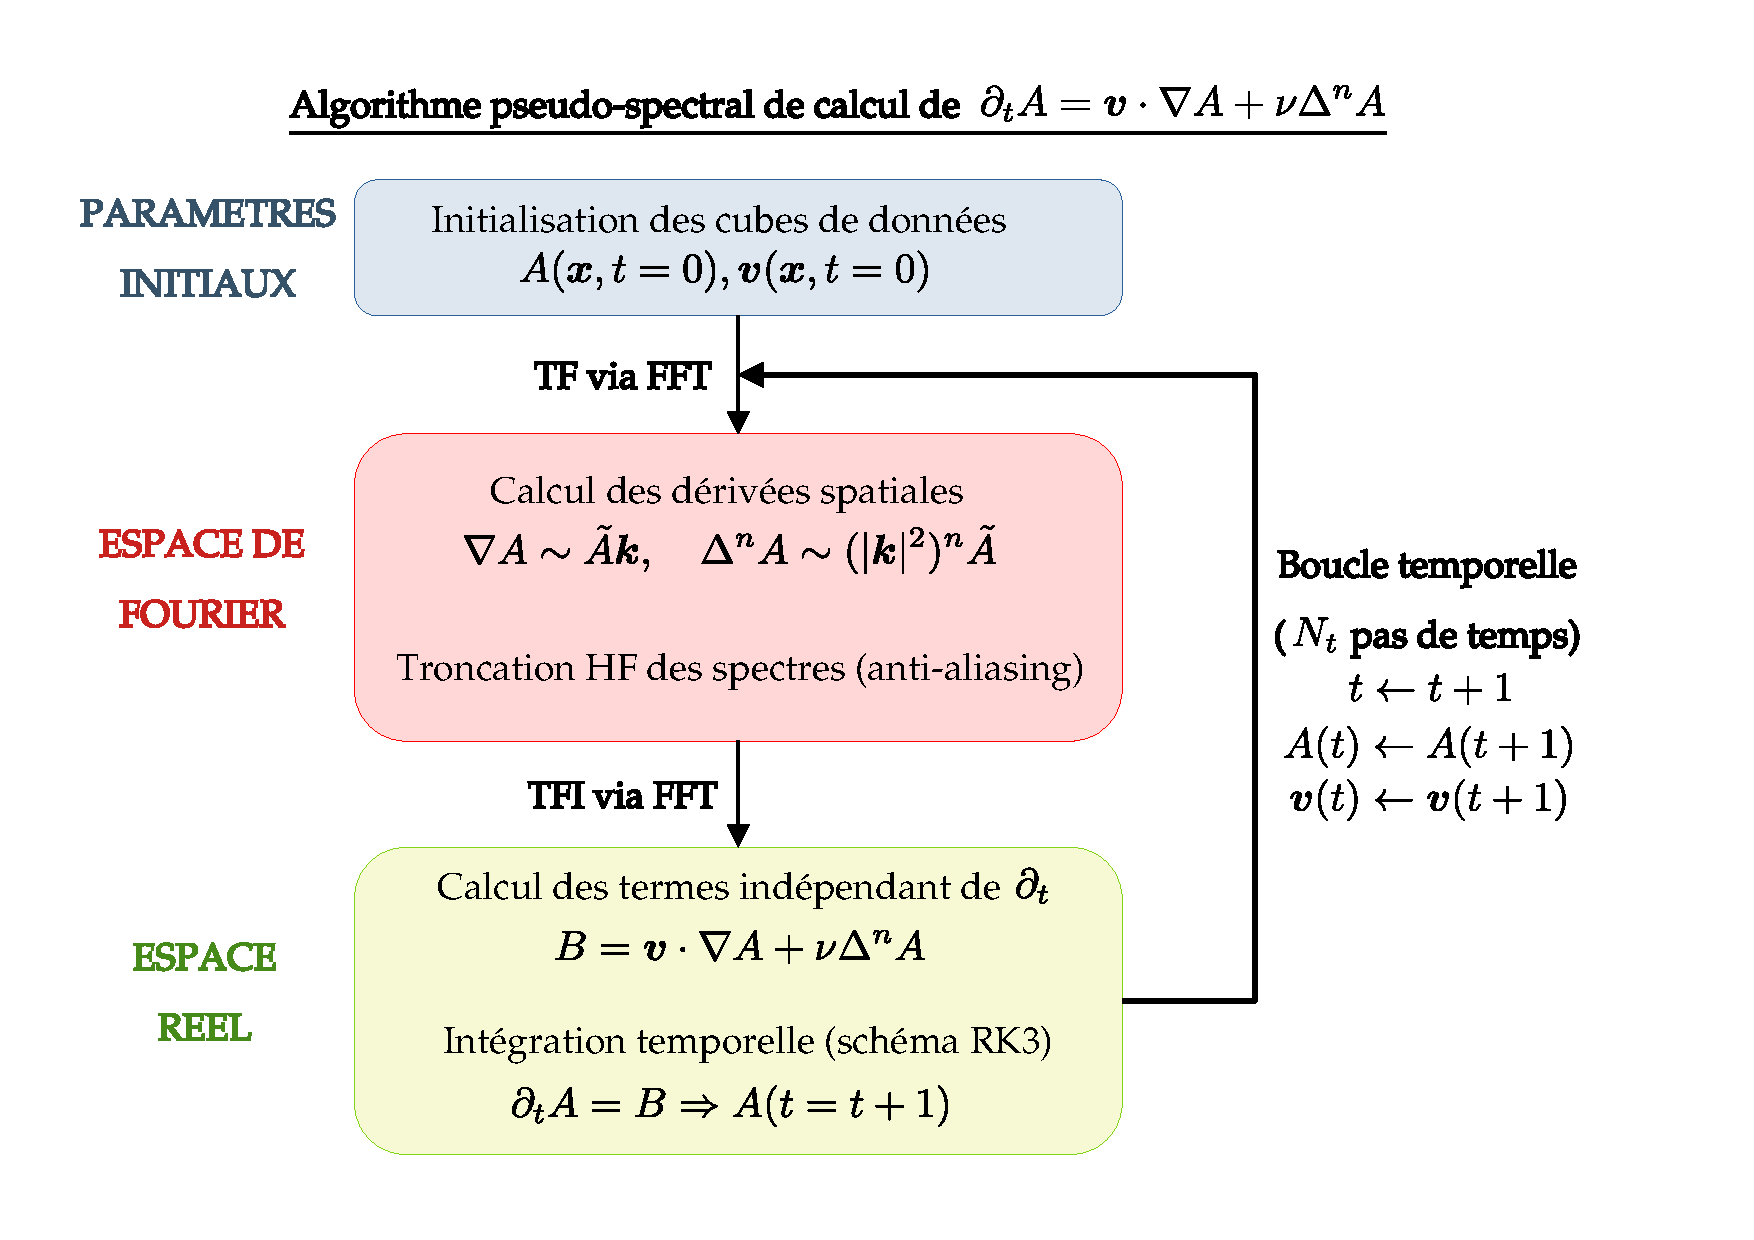
\includegraphics[width=0.9\linewidth,trim=1cm 1cm 3cm 1cm, clip=true]{./Mainmatter/Part_3/images_ch1/code_OCA}
\cprotect\caption{Algorithme d'intégration d'une équation d'évolution générique via une méthode pseudo-spectrale. Prise en compte des corrections d'anti-aliasing et d'hyperdissipation \ensuremath{\nu \Delta^n A}. TF(I) correspond à transformée de Fourier (inverse). }
\label{fig:algo_OCA}
\end{figure}

 Afin de limiter l'apparition de fort gradients et autres discontinuités liées à des instabilités numériques et induisant un arrêt brusque de la simulation, deux possibilités existent : appliquer un filtre passe-bas sur le spectre de la quantité impliquée ou un terme d'hyperviscosité dans son équation. Le choix effectué est celui de l'hyperviscosité, c'est-à-dire imposer une décroissance graduelle et de plus en plus intense du spectre de la quantité (pour plus d'informations, se référer à [\cite{borue_forced_1995,frisch_hyperviscosity_2008}]). Ce terme de dissipation numérique s'écrit $\nu \Delta^{n} X$ pour un champ $X$, avec $\nu$ une constante choisie initialement et $n$ un entier fixé à 4. $\Delta^{n}$ est effectué dans l'espace de Fourier où une décroissance du spectre en $\boldsymbol{k}^{-8}$ est donc obtenue.   
 L'existence d'un champ magnétique moyen dans les simulations induit une anisotropie spatiale de la turbulence. Sa direction est imposée suivant $\boldsymbol{e_z}$. Afin de refléter cette anisotropie, l'hyperviscosité est adaptée avec un paramètre $\alpha$ : $\Delta^{n}$ est calculé dans l'espace de Fourier tel que $(k^2_x +  k^2_y + \alpha k^2_z)^n$. Les paramètres $\nu$ et $\alpha$ sont résumés dans la \tabref{tab:setups_hd}. Avec le pas de temps $\delta t$, ils sont accordés empiriquement afin de réduire le temps de calcul, de maintenir la dissipation aux vecteurs d'onde les plus grands et d'éviter tout emballement de la simulation et l'apparition d'instabilités numériques. En termes de turbulence, l'hyperviscosité sera considérée comme le terme de dissipation évacuant l'énergie aux petites échelles.
 
 La cascade d'énergie est entretenue par un forçage permanent\footnote{Dans [\cite{hellinger_von_2018}, \cite{gomez_parallel_2005}, \cite{mininni_hybrid_2011}], une autre méthode est utilisée pour obtenir le développement d'une cascade turbulente : leurs champ de vitesse et champ magnétique sont initialisés par une superposition de modes de phases aléatoires, puis leurs simulations évoluent librement (simulations en déclin).}. Ce forçage de type antenne de Langevin (oscillateur harmonique forcé aléatoirement [\cite{tenbarge_oscillating_2014}]) injecte la somme de deux ondes de fréquences aléatoires mais proches de celle de l'onde d'Alfvén cinétique avec une amplitude correspondand au paramètre $A_f$ multiplié par un facteur aléatoire. Il est  
appliqué sur le champ de vitesse de sorte à maintenir la somme des énergies cinétique et magnétique perpendiculaires moyennes sous un niveau $E_{sup}$ et au-dessus d'un niveau $E_{inf}$ proche de $E_{sup}$. L'énergie moyenne totale est donc quasi-constante. 
Dans l'espace de Fourier, il prend la forme d'un peigne de distributions de Dirac non nulles aux vecteurs d'ondes les plus petits, tels que $\boldsymbol{k} = \{(0,\pm 1, \pm 1);(\pm 1,\pm 1, \pm 1)\}$ dans la grille numérique associée à l'espace de Fourier. L'angle d'injection de l'énergie, $\theta_i$, sert à définir la forme de la grille spatiale, un parallélépipède allongé dans la direction $\boldsymbol{e_z}$, la taille physique de cette grille est fixée telle que $L_{\perp}/L_z = \tan \theta_i$ avec $L_{\perp} = \frac{2 \pi}{k_{0\perp}} $.
 
 La taille de l'espace des échelles accessibles via ces simulations dépend de la taille de la grille spatiale. L'échelle la plus petite dans une direction est la distance minimale entre deux points de la grille dans cette direction, et l'échelle la plus grande est la moitié de la taille de la grille. Pour une étude de turbulence, on a besoin de plusieurs ordres de grandeur entre les échelles minimales et maximales. Afin d'obtenir un nombre de points suffisant, on part d'une grille de taille physique fixée mais contenant peu de points, par exemple $128^3$, puis, après avoir atteint un régime turbulent satisfaisant tel que les spectres soient stabilisés, on augmente le nombre de points et ainsi de suite jusqu'à avoir la taille voulue pour l'espace des échelles et un spectre stable. Le nombre de points idéal serait $1024^3$ ou plus, mais plus il y a de points, plus le temps de calcul augmente\footnote{Typiquement, il faut environ un mois de calcul avec $64$ processeurs pour obtenir une simulation de taille $512^2\times 1024$ dans laquelle la turbulence se serait a priori entièrement développée} et plus le calcul monopolisera de la mémoire. Similairement, le calcul du taux de cascade sera aussi plus contraignant. Un compromis doit donc être trouvé. La taille de cube minimale considérée dans le cadre des études de turbulence sera $512^3$ et une partie des simulations aura une résolution de $512^2$ dans le plan $\{\boldsymbol{e_x},\boldsymbol{e_y}\}$ et $1024$ dans la direction $\boldsymbol{e_z}$. 
 
 Les simulations utilisées et détaillées dans la \tabref{tab:setups} et la \tabref{tab:setups_hd} ont, pour la plupart, fait l'objet de l'article [\cite{ferrand_fluid_2021}]. Parmi elles, une est de résolution $1024^3$. Elle ne sera pas traitée ici car sa taille est trop importante pour le code de post-traitement implémenté et les moyens de calcul à disposition (mésocentre). 
 
 \section{Code de post-traitement pour le calcul numérique de lois exactes }
 \label{sec-312}
 
 On a vu qu'une loi exacte est une formule statistique donnant un résultat en fonction de l'échelle $\boldsymbol{\ell}$. Elle dépend de quantités évaluées localement en deux points puis combinées en une expression qui est ensuite moyennée. Une partie des termes doit ensuite être dérivée dans l'espace des échelles si aucune hypothèse d'intégration n'est effectuée. Cette méthode pourrait être implémentée directement. On considèrerait les quantités à disposition, a priori des cubes évalués en $\boldsymbol{x}$), on les translaterait de sorte à obtenir des cubes évalués en $\boldsymbol{x} - \boldsymbol{\ell}$, puis on les combinerait suivant l'expression voulue avant de les moyenner. On obtiendrait ainsi notre résultat évalué en un point de l'espace des échelles et il faudrait recommencer encore et encore afin d'obtenir l'ensemble de l'espace des échelles. Enfin, on dériverait ou intégrerait le résultat. Cet algorithme est schématisé sur la \figref{fig:algo_direct}.
 \begin{figure}[!ht]
  \centering
 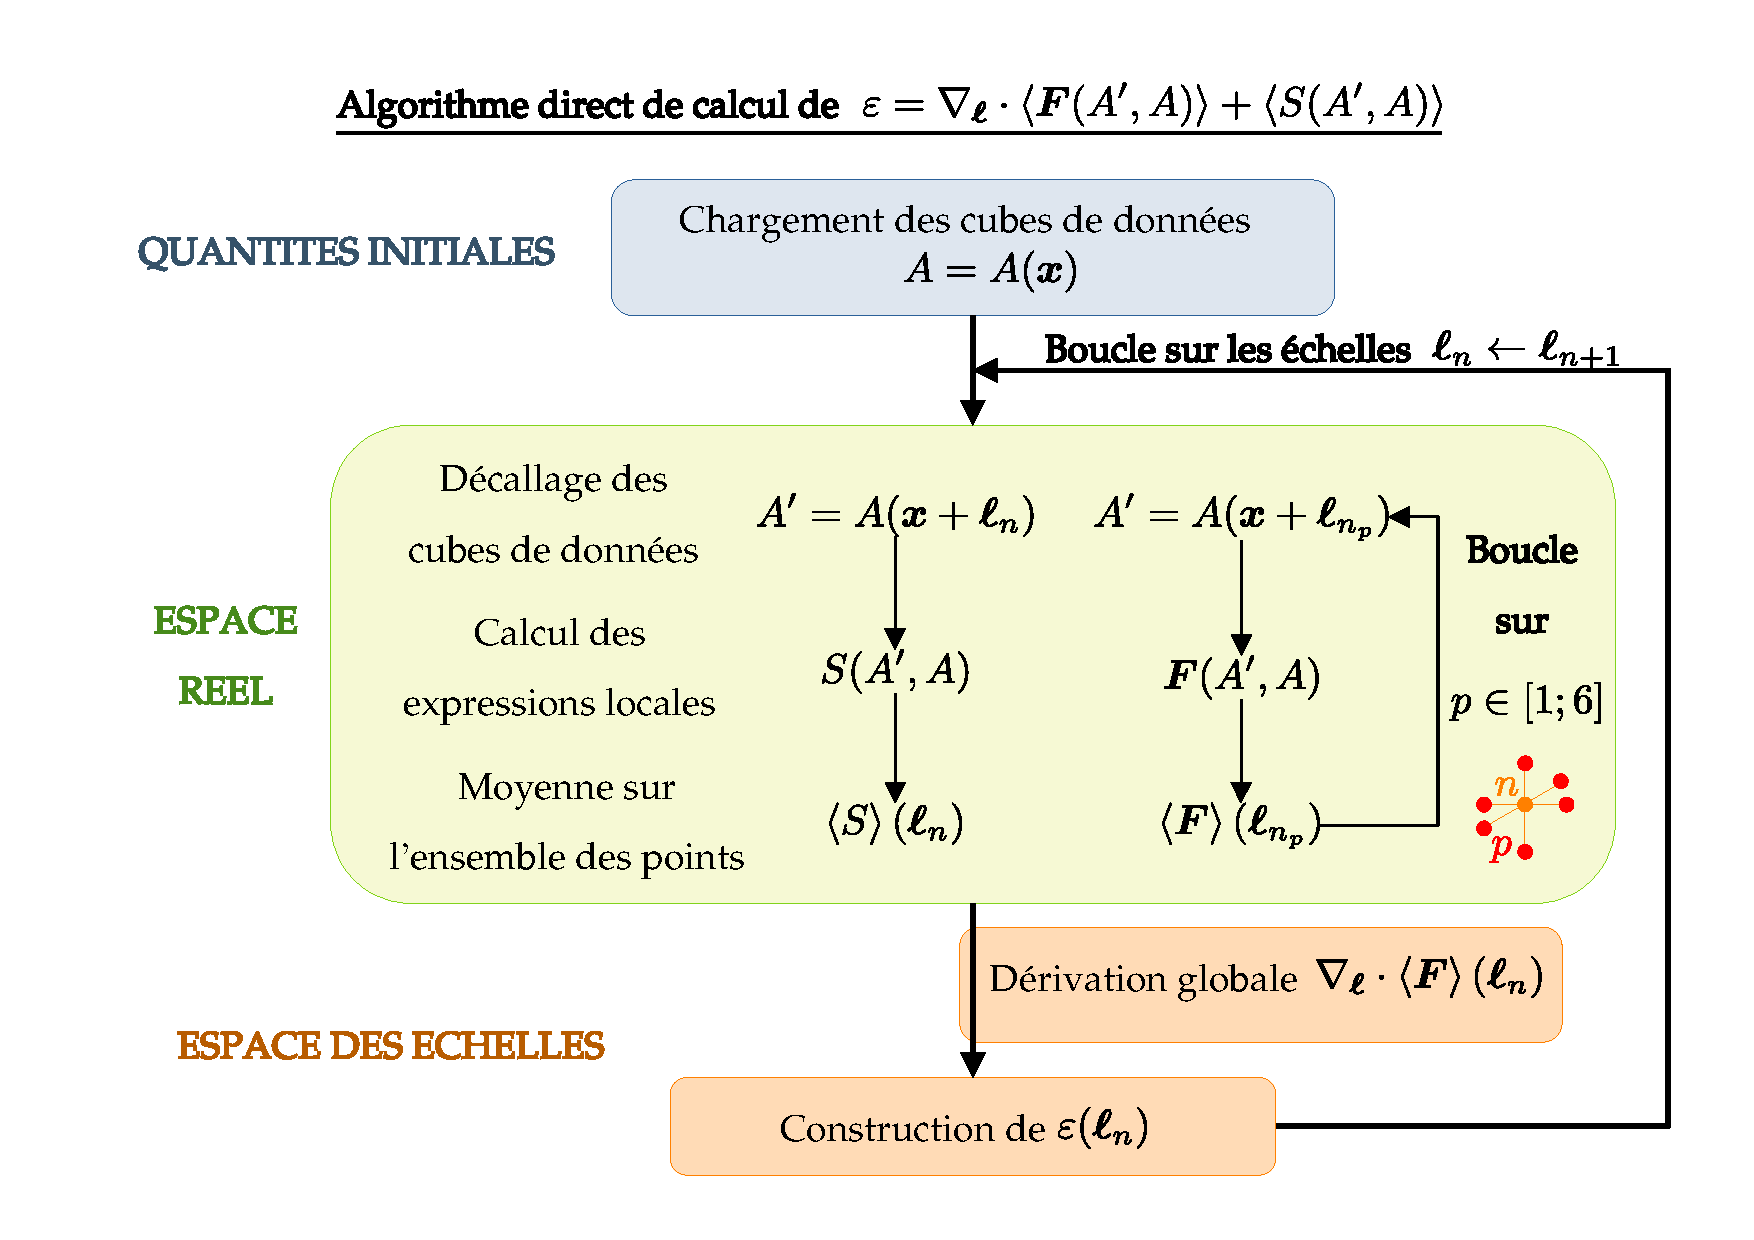
\includegraphics[width=0.9\linewidth,trim=2cm 1cm 1cm 1cm, clip=true]{./Mainmatter/Part_3/images_ch1/code_EL_direct}
 \cprotect\caption{Algorithme de calcul du taux de cascade \ensuremath{\varepsilon} via la méthode directe. Les quantités impliquées sont des quantités génériques.}
 \label{fig:algo_direct}
 \end{figure}
 
 Cette méthode est coûteuse en temps de calcul et demande des compromis. Pour réduire le temps de calcul, on peut choisir intelligemment un certain nombre de vecteurs d'échelle. Tout d'abord, on peut jouer sur la parité de la loi exacte et ne calculer que les vecteurs tels que $\ell_z \leq 0$.  \cite{ferrand_fluid_2021} et \cite{ferrand_-depth_2022} par exemple, utilisent les hypothèses d'isotropie ou d'axisymétrie de l'espace d'échelles. Dans le cas isotrope, l'espace des échelles est alors vu comme une sphère avec 73 vecteurs directeurs partant de son centre. Dans le cas axisymétrique, le découpage est similaire, mais effectué dans des disques pour chaque $\ell_z$. La divergence dans l'espace des échelles est ensuite effectuée sphériquement (resp. cylindriquement) le long de $\ell = |\boldsymbol{\ell}|$ (resp. $\ell_{\perp} = \sqrt{\ell^2_x + \ell^2_y}$) en supposant les dérivées angulaires nulles. Je n'ai pas voulu faire de même, n'étant pas convaincue de l'indépendance angulaire de la dérivée et trouvant la statistique finale faible. Une autre possibilité est de choisir les vecteurs en fonction du mode de représentation final. Si ce mode de représentation est logarithmique, on peut ne choisir qu'un nombre limité de vecteurs à grande échelle tels qu'ils soient régulièrement espacés en représentation logarithmique [\cite{manzini_local_2022}]. Un problème de cette méthode est l'irrégularité de la grille résultante. La divergence dans l'espace des échelles doit donc se faire vecteur par vecteur à partir des six échelles les plus proches (au minimum). Ce choix-là ne semblait toujours pas satisfaisant, car il implique de devoir potentiellement refaire le calcul en fonction du mode de représentation final et un biais apparaît en cas de moyenne dans l'espace des échelles. Ces compromis doivent en plus être accompagnés d'une optimisation, voire d'une parallélisation du calcul numérique. 
 
 Après maintes versions et tentatives d'optimisation de mon code de post-traitement, codé en \verb|Python| et essayant de respecter explicitement la forme de la loi exacte, j'ai décidé de changer radicalement de point de vue. 
 Mathématiquement, les opérations de corrélation et de convolution, $*$, sont liées. En effet, si l'on considère deux quantités réelles $s$ et $r$, leur fonction de corrélation peut s'écrire :
 \begin{eqnarray}
      C_{s,r}(\boldsymbol{\ell})  &=& \frac{1}{V}\iiint_V s(\boldsymbol{x} + \boldsymbol{\ell}) r (\boldsymbol{x}) d\boldsymbol{x} =  \frac{1}{V} \iiint_V s(\boldsymbol{x}) r (\boldsymbol{x} - \boldsymbol{\ell}) d\boldsymbol{x} \nonumber\\
      &=&  \frac{1}{V} \iiint_V s(\boldsymbol{x}) r (-(\boldsymbol{\ell}-\boldsymbol{x}) ) d\boldsymbol{x} = \left[ \frac{1}{V} s * \mathcal{\hat{P}}r \right](\boldsymbol{\ell}),
 \end{eqnarray}
 avec $V$ le volume d'intégration et $\mathcal{\hat{P}}$ l'opérateur de parité.
 Ainsi appliquer l'opération de corrélation entre $s$ et $r$ revient à convoluer $s$ évaluée en $\boldsymbol{x}$ avec $r$ évaluée en $-\boldsymbol{x}$.
 Une autre propriété mathématique intéressante est que l'opération de convolution correspond à un simple produit dans l'espace de Fourier et que $\mathcal{\hat{P}}r$ correspond au conjugué, $(\widetilde{r})^*$, de $\widetilde{r}$ la transformée de Fourier de $r$. Ainsi en notant $\widetilde{C}_{s,r}$ la transformée de Fourier de $C_{s,r}$ et $\text{TFI}[.]$ la transformée inverse, on obtient : 
\begin{eqnarray}
    C_{s,r}(\boldsymbol{\ell})  = \text{TFI}[\widetilde{C}_{s,r}] =  \frac{1}{V}\text{TFI}[\widetilde{s} (\boldsymbol{k}) ( \widetilde{r})^*(\boldsymbol{k})]. \quad
\end{eqnarray}
L'obtention de l'ensemble de l'espace des échelles est donc possible mais demande de développer tous les termes factorisés de la loi exacte. Par exemple, pour la fonction de structure $\left<\delta \boldsymbol{v} \cdot \delta \boldsymbol{v} \delta \boldsymbol{v}\right> $ :
\begin{eqnarray}
    \left<\delta \boldsymbol{v} \cdot \delta \boldsymbol{v} \delta \boldsymbol{v}\right> &=& \left<\boldsymbol{v'} \cdot \boldsymbol{v'} \boldsymbol{v'} - \boldsymbol{v} \cdot \boldsymbol{v} \boldsymbol{v}  + \boldsymbol{v} \cdot \boldsymbol{v} \boldsymbol{v'} + 2 \boldsymbol{v'} \cdot \boldsymbol{v} \boldsymbol{v}- \boldsymbol{v'} \cdot \boldsymbol{v'} \boldsymbol{v} - 2 \boldsymbol{v'} \cdot \boldsymbol{v} \boldsymbol{v'}\right> \nonumber\\
&=&  \text{TFI} [\widetilde{C}_{\boldsymbol{v},\boldsymbol{v} \cdot \boldsymbol{v}} - \widetilde{C}_{\boldsymbol{v} \cdot \boldsymbol{v},  \boldsymbol{v}} + 2 \widetilde{C}_{\boldsymbol{v},\boldsymbol{v}\boldsymbol{v}}  - 2 \widetilde{C}_{\boldsymbol{v}\boldsymbol{v},\boldsymbol{v}} ] \quad \nonumber  \\
&=& \frac{1}{N}  \text{TFI} [   (\widetilde{ \boldsymbol{v} \cdot \boldsymbol{v}})(\boldsymbol{\widetilde{v}})^* - \boldsymbol{\widetilde{v}} (\widetilde{\boldsymbol{v} \cdot \boldsymbol{v}})^* +2\boldsymbol{\widetilde{v}}^* \cdot (\widetilde{\boldsymbol{v} \boldsymbol{v}}) -2\boldsymbol{\widetilde{v}}\cdot (\widetilde{\boldsymbol{v} \boldsymbol{v}})^* ], \quad
\end{eqnarray}
avec $C_{\boldsymbol{v} \cdot \boldsymbol{v},  \boldsymbol{v}} = \left< \boldsymbol{v'} \cdot \boldsymbol{v'} \boldsymbol{v}\right>$, $C_{\boldsymbol{v}\boldsymbol{v},\boldsymbol{v}} = \left< \boldsymbol{v'} \cdot \boldsymbol{v} \boldsymbol{v'} \right>$ et $N$ le nombre de points moyennés (volume discret), tout en sachant que par homogénéité statistique, on a $\left< \boldsymbol{v'} \cdot \boldsymbol{v'} \boldsymbol{v'}\right> = \left< \boldsymbol{v} \cdot \boldsymbol{v} \boldsymbol{v}\right>$ et que la moyenne est distributive. Cette méthode est utilisable car il est possible de développer les expressions en des produits de deux quantités générales, une évaluée au point $\boldsymbol{x}$ et l'autre en $\boldsymbol{x'}$, et parce que la simulation est périodique. L'algorithme associé à cette méthode est schématisé sur la \figref{fig:algo_spec}.
 \begin{figure}[!ht]
  \centering
 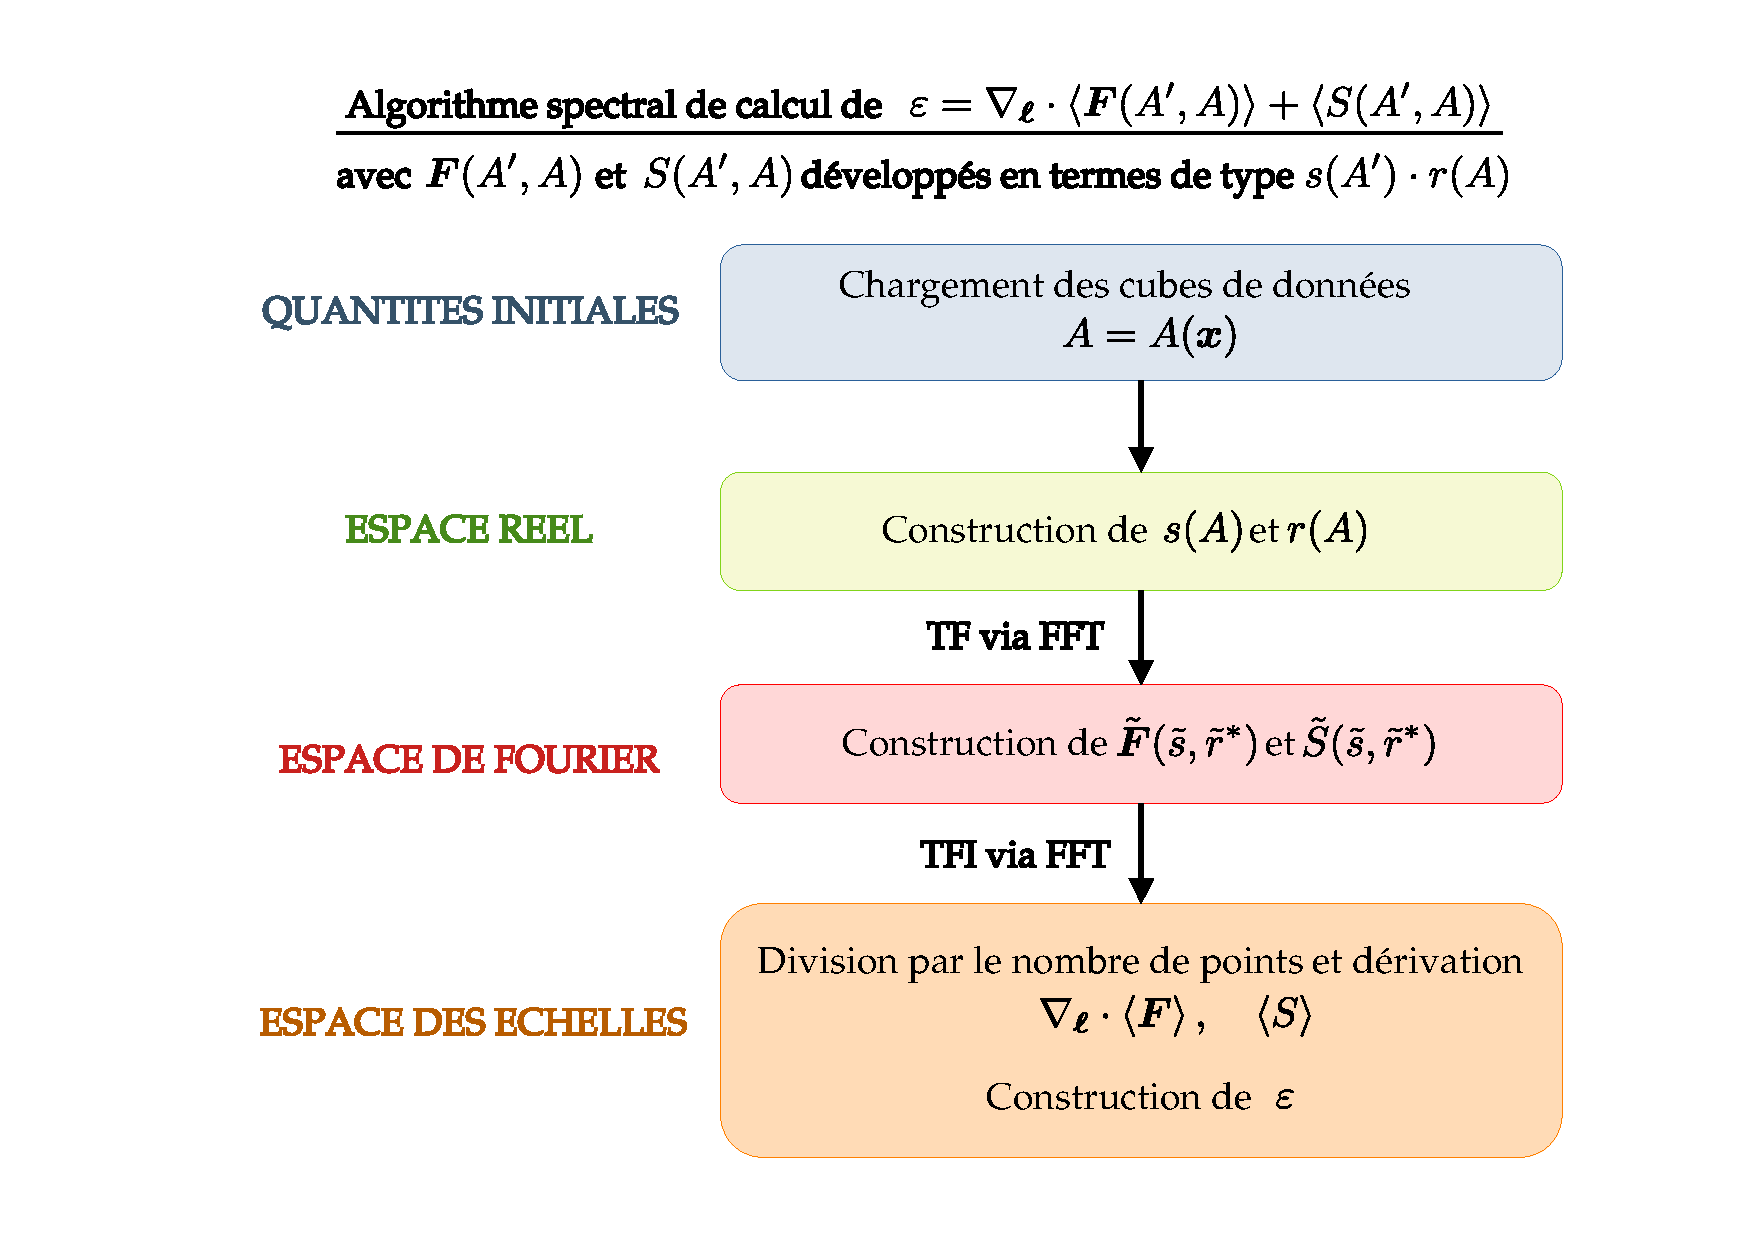
\includegraphics[width=0.93\linewidth,trim=4cm 1cm 3cm 1cm, clip=true]{./Mainmatter/Part_3/images_ch1/code_EL_spec}
 \cprotect\caption{Algorithme de calcul du taux de cascade \ensuremath{\varepsilon} via la convolution. Les quantités impliquées sont des quantités génériques.}
 \label{fig:algo_spec}
 \end{figure}
 Il demande quelques précautions lors de son implémentation, car il peut vite devenir coûteuse en mémoire, l'ensemble des termes présents dans une loi exacte devant être développé. Cependant, elle permet d'obtenir un résultat complet, indépendant du mode de représentation final des résultats. C'est donc la méthode qui a été choisie. De plus, en usant de l'algorithme de \cacro{FFT}, elle s'avère particulièrement rapide (moins de dix minutes pour calculer séparément les trois termes de \cacro{PP98} pour CGL2 par exemple).
 
 \section{Mode de représentation du résultat}
 \label{sec-313}
 \begin{figure}[!ht]
  \centering
 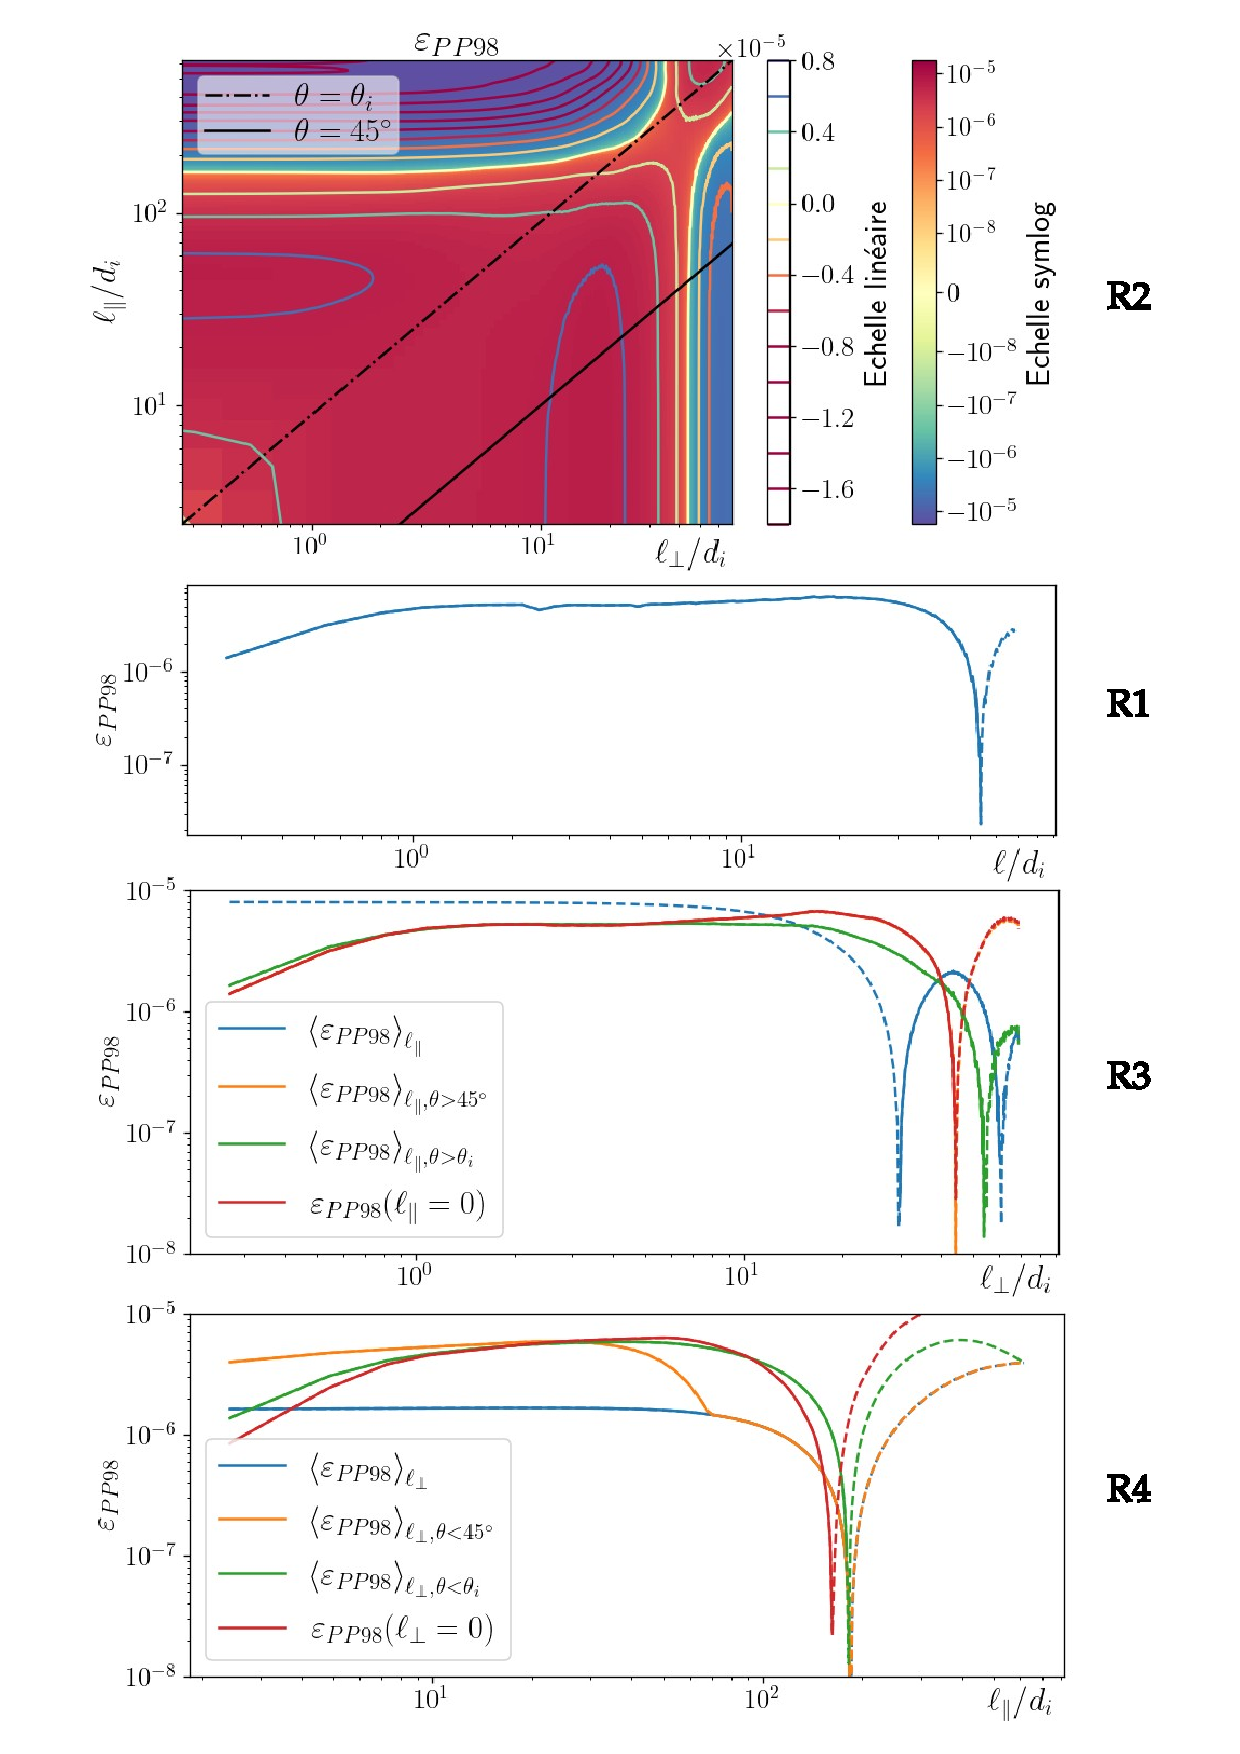
\includegraphics[width=0.75\linewidth,trim=1cm 0.5cm 1cm 0.5cm, clip=true]{./Mainmatter/Part_3/images_ch1/rep_CGL1}
 \cprotect\caption{Différents modes de représentations du taux de cascade \ensuremath{\varepsilon_{PP98}} calculé avec \cacro{PP98} dans les données de la simulation CGL1. R2 : \cacro{2D} en fonction de \ensuremath{\ell_{\perp}} et \ensuremath{\ell_{\parallel}}, avec deux échelles de couleurs, une échelle symlog, linéaire entre \ensuremath{-10^{-8}} et \ensuremath{10^{-8}} (barre de couleur continue), et une échelle linéaire (barre de couleur discontinue) et les frontières \ensuremath{\theta = \theta_i} (noire discontinue) et \ensuremath{\theta = \ang{45}} (noire continue). R1 : \cacro{1D} en fonction de \ensuremath{\ell}. R3 : \cacro{1D} en fonction de \ensuremath{\ell_{\perp}}, pour \ensuremath{\ell_{\parallel} = 0} (rouge), moyenne sur l'ensemble des \ensuremath{\ell_{\parallel}} (bleue), moyennes sur les \ensuremath{\ell_{\parallel}} tels que \ensuremath{\theta > \ang{45}} (orange) et \ensuremath{\theta > \theta_i} (vert). R4 : \cacro{1D} en fonction de \ensuremath{\ell_{\parallel}}, pour \ensuremath{\ell_{\perp} = 0} (rouge), moyenne sur l'ensemble des \ensuremath{\ell_{\perp}} (bleue), moyenne sur les \ensuremath{\ell_{\perp}} tels que \ensuremath{\theta < \ang{45}} (orange) et \ensuremath{\theta < \theta_i} (vert). Le caractère continu ou discontinu des courbes \cacro{1D} reflète le signe de \ensuremath{\varepsilon_{PP98}}.}
 \label{fig:rep_CGL1}
 \end{figure}
 Le résultat de l'algorithme de calcul par convolution est, pour chaque quantité, un parallélépipède couvrant une gamme d'échelles physiques dans la direction $\boldsymbol{e_z}$ différente de la gamme d'échelles couverte dans les directions perpendiculaires, $\boldsymbol{e_x}$ ou $\boldsymbol{e_y}$.  
 Ces gammes d'échelles couvrant différents ordres de grandeur, une représentation logarithmique est usuellement adoptée. Le caractère tridimensionnel de la grille parallélépipédique impose de choisir une méthode de réduction (\cacro{3D} vers \sacro{2D} ou \cacro{1D}) afin de pouvoir visualiser facilement les quantités. Différents types de réduction sont possibles et illustrés sur la \figref{fig:rep_CGL1} : 
 
\begin{itemize}
    \item R1 : \cacro{1D} en fonction de $\ell = |\boldsymbol{\ell}|$, en moyennant la quantité sur des coquilles de rayon moyen $\ell$,
    \item R2 : \sacro{2D} en fonction de $\ell_{\perp} = \sqrt{\ell_x^2 + \ell_y^2}$ et $\ell_{\parallel} = \ell_z$, en moyennant la quantité sur des couronnes de rayon moyen $\ell_{\perp}$ dans chaque plan perpendiculaire à $\boldsymbol{e_z}$,
    \item R3 : \cacro{1D} en fonction de $\ell_{\perp}$, en moyennant la quantité sur des coquilles cylindriques de rayon moyen $\ell_{\perp}$, la moyenne suivant $\ell_{\parallel}$ peut s'effectuer de diverses manières qui seront détaillées par la suite,
    \item R4 : \cacro{1D} en fonction de $\ell_{\parallel}$ en moyennant chaque plan perpendiculaire à $\boldsymbol{e_z}$, la moyenne suivant $\ell_{\perp}$ peut s'effectuer de diverses manières qui seront détaillées par la suite. 
\end{itemize}
 
 Sachant que la grille parallélépipédique couvre des gammes d'échelles différentes dans la direction $\boldsymbol{e_z}$ et les directions perpendiculaires (voir la carte R2 sur la \figref{fig:rep_CGL1}), notre géométrie est fondamentalement axisymétrique. La représentation de type R2 est donc la plus adaptée. L'échelle \og symlog \fg{}\footnote{Cette échelle décrit l'ensemble des nombres réels via trois représentations : $[x_0;+\infty[$ en représentation logarithmique, $]-x_0;x_0[$ en représentation linéaire (afin d'éviter la singularité du point 0), puis  $]-\infty; -x_0]$ en représentation logarithmique (en prenant l'opposé du logarithme de la valeur absolue). $x_0$ est choisi le plus petit possible.} permet de repérer les changements de signe et les ordres de grandeur couverts par $\varepsilon_{PP98}$ tandis que les courbes de niveau linéaires révèlent les variations plus spécifiques telles qu'un affaiblissement aux petites échelles ou des bosses (courbes de niveau bleues) aux échelles parallèles et perpendiculaires intermédiaires. On pourrait définir une zone inertielle entre les courbes de niveau associées à la valeur $\num{0.4}$. On remarque que cette zone semble carrée, cela est dû aux axes logarithmiques. Avec des axes linéaires, on observerait un quart d'ellipse liant $\ell_{\parallel}/d_i = \num{1e2}$ à $\ell_{\perp}/d_i \simeq \num{30} $. Le problème des cartes est la difficulté de comparer de multiples quantités. Une représentation \cacro{1D} sera donc nécessaire.

 R1 peut donner un résultat biaisé. Ainsi, sur le graphique R1 de la \figref{fig:rep_CGL1}, le résultat correspond quasiment entièrement (sauf aux très grandes échelles communes aux directions parallèle et perpendiculaire) à $\varepsilon_{PP98} (\ell_{\parallel} = 0)$ (en rouge sur le graphique R3 de la \figref{fig:rep_CGL1}). Le manque de points pour effectuer la moyenne en chaque $\ell$, induit des variations non-physiques du résultat (sursauts à intervalles réguliers sur le graphique R1 de la \figref{fig:rep_CGL1}). R3 ou R4 sont peut-être plus adaptés même si le caractère petit ou grand des échelles est défini à partir de $\ell=|\boldsymbol{\ell}|$ (resp. petit ou grand). 
 
 Cependant, visualiser la cascade via R3 en moyennant l'ensemble des $\ell_{\parallel}$ à $\ell_{\perp}$ fixé (courbe bleue) vient mixer les petits et grands $\ell$. La zone négative à grand $\ell_{\parallel}$ vient alors écraser la zone inertielle présumée et plus encore la variation des petites échelles. Le même phénomène apparaît pour R4 (courbes bleues sur les graphiques R3 et R4 de la \figref{fig:rep_CGL1}). Une autre possibilité de réduction serait de ne regarder qu'une direction $\ell_{\parallel} = 0$ pour R3 ou $\ell_{\perp} = 0$ pour R4 (courbes rouges sur les graphiques R3 et R4 de la \figref{fig:rep_CGL1}). Le résultat n'est alors pas très lisse et peu représentatif de la variation d'ensemble. 

 La troisième possibilité correspond à appliquer un filtre angulaire. En définissant $\theta$, l'angle entre $\boldsymbol{\ell}$ et $\boldsymbol{e_z}$, on pourrait considérer que les $\boldsymbol{\ell}$ contribuant à la dynamique parallèle sont les $\boldsymbol{\ell}$ quasi-parallèles tels que $\theta < \ang{45}$, et ceux contribuant à la dynamique perpendiculaire les $\boldsymbol{\ell}$ quasi-perpendiculaires tels que $\theta < \ang{45}$. La frontière $\theta = \ang{45}$ est représentée par une ligne noire continue sur la carte R2 de la \figref{fig:rep_CGL1}, et les résultats apparaissent en orange sur les graphiques R3 et R4. Pour R3, le résultat coïncide avec $\varepsilon_{PP98} (\ell_{\parallel} = 0)$. En effet, aux petites échelles, le plan tel que $\ell_{\parallel} = 0$ est la seule contribution à la moyenne. Similairement, pour R4, on assiste à un écroulement de la courbe qui rejoint $\left< \varepsilon_{PP98} \right>_{\ell_{\perp}}$ en $\ell_{\parallel} = \num{7e1}$. Cet écroulement est dû à la prise en compte de la région bleue à droite de la carte R2 pour les échelles supérieures à $\num{7e1}$. Ce filtre angulaire n'est donc pas adapté.
 
 La réduction \cacro{1D} qui sera adoptée par la suite correspond à un filtrage angulaire basé sur l'angle d'injection de l'énergie $\theta_i$. Ce dernier impose la géométrie de la grille et les gammes d'échelles accessibles. Dans l'espace des échelles, l'injection a lieu aux échelles telles que $\ell$ est maximal, c'est-à-dire dans l'angle supérieur droit de la carte R2 \figref{fig:rep_CGL1}. $\theta = \theta_i$ correspond à la diagonale représentée par une ligne noire discontinue. Appliquer cette réduction nous donne les courbes vertes des graphiques R3 et R4 de la \figref{fig:rep_CGL1}. N'y apparaissent, ni les artéfacts visibles avec R1, ni les saturations visibles sur les courbes bleues ou oranges, et elles sont plus représentatives du comportement de $\varepsilon_{PP98}$ dans l'ensemble de l'espace des échelles que les courbes rouges. On remarquera tout de même que la décroissance en allant vers les petites échelles est moins accentuée que pour les courbes rouges : les premières échelles de $\ell_{\parallel}$ (resp. $\ell_{\perp}$) différentes de $\num{0}$ sont prises en compte dans la moyenne des premiers points de $\varepsilon_{PP98}$ en fonction de $\ell_{\perp}$ (resp. $\ell_{\parallel}$).
 
%\newpage
 \section{Synthèse des méthodes et choix numériques}
 \label{synt-31}
\fcolorbox{blue}{white}{\begin{minipage}[c]{\linewidth}

\paragraph{\\Code de simulation d'un plasma turbulent (\texttt{Fortran}) : }
\begin{itemize}
\item Méthode d'intégration pseudo-spectrale (voir \figref{fig:algo_OCA}) des équations fluides.
\item Des termes d'hyperdissipation qui joueront le rôle de la dissipation aux petites échelles.
\item Un forçage permanent (dans l'espace de Fourier) de fréquences aléatoires proches de la pulsation Alfvénique et maintenant l'énergie perpendiculaire (cinétique + magnétique) du système quasiment constante.
\item Une géométrie périodique dépendant de l'angle d'injection de l'énergie $\theta_i$ et de la résolution de la grille numérique. \\
\end{itemize}
Je n'ai pas participé à l'écriture de ce code mais je l'ai utilisé pour compléter le lot de simulations analysé par \cite{ferrand_fluid_2021}.
\end{minipage}}

\fcolorbox{red}{white}{\begin{minipage}[c]{\linewidth}
\paragraph{\\Calcul des termes des lois exactes (\texttt{Python/Numpy/Scipy}) : }
Obtention rapide de {\bf l'ensemble de l'espace d'échelles accessible} grâce à une méthode de calcul spectrale basée sur le lien entre corrélation et convolution et sur la périodicité des simulations. L'algorithme est schématisé sur la \figref{fig:algo_spec}.

\paragraph{\\Visualisation des résultats (\texttt{Python/Matplotlib}) : représentation cylindrique} 
\begin{itemize}
\item Représentation \sacro{2D} en fonction de $\ell_{\parallel}$ et $\ell_{\perp}$ avec des échelles de couleurs de type chaud/froid (indiquant facilement le signe du résultat) associées aux variations logarithmiques (fond) et linéaires (courbes de niveaux) du résultat. 
\item Représentation \cacro{1D} en fonction de $\ell_{\perp}$. Réduction du résultat \sacro{2D} en moyennant sur $\ell_{\parallel}$ pour $\theta > \theta_i$.
\item Représentation \cacro{1D} en fonction de $\ell_{\parallel}$. Réduction du résultat \sacro{2D} en moyennant sur $\ell_{\perp}$ pour $\theta < \theta_i$. 
\end{itemize} 
Avec $\theta$ l'angle entre $\boldsymbol{\ell}$ et la direction moyenne du champ magnétique $\boldsymbol{e_z}$. \\

J'ai implémenté les codes de post-traitement et de visualisation des termes des lois exactes. Le code de post-traitement est disponible sur [GitHub : \cite{noauthor_paulinesimon972022-07_simu_exact_laws_nodate}].
\end{minipage}}


  Avant d'attaquer les spécificités des modèles simulés et les lois exactes associées, il est nécessaire de valider les méthodes numériques exposées dans le Chapitre \ref{ch-31} et d'en déterminer les biais. Dans la section \ref{sec-321}, les résultats de la loi exacte \cacro{IMHDH} seront comparés aux résultats de \cacro{F21}. %Dans la section \ref{sec-323}, les résultats \acs{MHD} avec pression isotrope dérivée dans le Chapitre \ref{ch-13} seront comparés aux prédictions de \ac{A18}. 
  Enfin, dans la section \ref{sec-323}, une méthode d'estimation de l'incertitude sur nos résultats sera proposée. 
  Les simulations utilisées dans ces études comparatives sont CGL1 et CGL3 (voir détail \tabref{tab:setups} et \tabref{tab:setups_hd}). Elles font partie des simulations du modèle \sacro{CGLHPe} analysées par \cacro{F21} et elles feront l'objet du Chapitre \ref{ch-33}.  

  
 
% Pour chaque simulation, une temps a été sélectionnée. À partir de cette temps, la simulation a été relancée sur quelques pas de temps rapprochés avec extraction des quantités pour chacun d'eux. Sauf exception de la  \figref{fig:compainc_t}, tous les résultats montrés dans ce chapitre correspondent à une moyenne de ces échantillons. Pour CGL1, la temps correspond au temps utilisé par F21, pour CGL3, c'est la temps précédente, \ac{F21} analysant le temps $t =\num{362}$ mais les lois exactes étant statistiquement stationnaire, on s'attend à retrouver des résultats similaires.    

 \section{Comparaison de résultats Inc-MHD-Hall avec pression isotrope et schémas numériques}
 \label{sec-321}
 
 \subsection{Comparaison avec des  résultats Inc-MHD-Hall}

 Afin de valider les méthodes et choix décrits dans le Chapitre \ref{ch-31}, nous avons calculé avec les données de CGL1 et CGL3 les quantités comparées par \cacro{F21} : 
 \begin{itemize}
     \item $\varepsilon_{MHD}$, provenant de la loi \cacro{PP98} (équation \eqref{eq:synth_inc_EL}),
     \item $\varepsilon_{Hall}$, la correction Hall incompressible (équation \eqref{eq:corr_hallinc}),
     \item $\varepsilon_{MHD-Hall} = \varepsilon_{MHD} + \varepsilon_{Hall}$, qui correspond au résultat de la loi \cacro{IMHDH} dérivée par \cite{ferrand_exact_2019}.
 \end{itemize} 
 Pour CGL1, le temps sélectionné, indiqué dans la \tabref{tab:setups}, est celui utilisée par \cacro{F21}. Ce n'est pas le cas pour CGL3, pour laquelle \cacro{F21} utilise $t =\num{357}$. Afin de ne pas apporter d'incertitude à notre comparaison en changeant les données utilisées, les résultats seront exceptionnellement donnés pour $t =\num{357}$ dans cette section. 
 
 Par conséquent, aucune différence que l'on pourra noter ne proviendra des données, des expressions des quantités ou de leur domaine de validité. Les différences entre les résultats résideront dans les schémas numériques utilisés. On a indiqué le nôtre par la mention \cacro{FEL} et celui de \cacro{F21} par \og F21\fg{}.  Nos résultats sont présentés sur la \figref{fig:compainc} par des lignes pleines et sont accompagnés de ceux des figures 3 et 5 de \cacro{F21} en pointillés. 
 
 \begin{figure}[!ht]
  \centering
 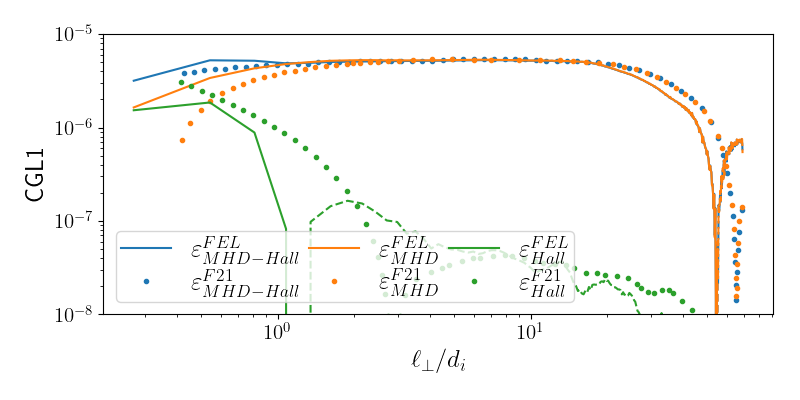
\includegraphics[width=0.85\linewidth,trim=0.5cm 0.5cm 0.5cm 0.5cm, clip=true]{./Mainmatter/Part_3/images_ch2/CGL1_compainc}
 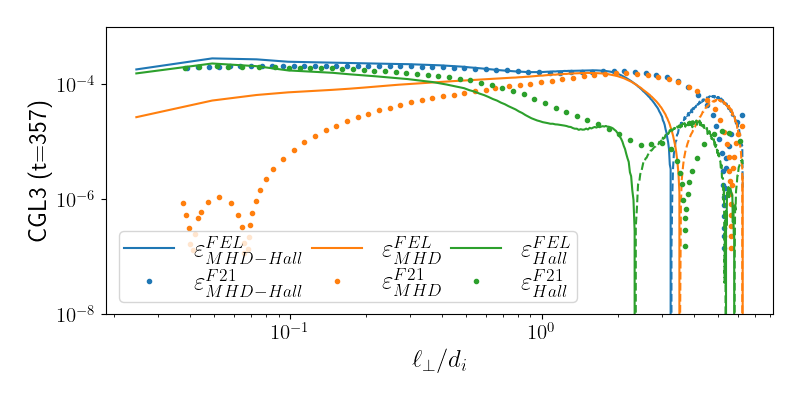
\includegraphics[width=0.85\linewidth,trim=0.5cm 0.5cm 0.5cm 0.5cm, clip=true]{./Mainmatter/Part_3/images_ch2/CGL3_compainc}
 \cprotect\caption{Mode de représentation : \cacro{1D} en fonction de \ensuremath{\ell_{\perp}} normalisé par \ensuremath{d_i}. Lignes pleines : nos résultats (avec en lignes discontinues les valeurs négatives). Pointillés : résultats extraits des figures 3 et 5 de \cacro{F21}. Bleu : \ensuremath{\varepsilon_{MHD-Hall}}. Orange : \ensuremath{\varepsilon_{MHD}}. Vert : \ensuremath{\varepsilon_{Hall}}. Haut : CGL1. Bas : CGL3 (\ensuremath{t =\num{357}}).}
 \label{fig:compainc}
 \end{figure}
 
 Tout d'abord, pour chaque simulation, on retrouve les points physiques attendus : 
 \begin{itemize}
     \item Pour CGL1 : une zone inertielle \cacro{MHD} telle que $\varepsilon_{MHD-Hall} = \varepsilon_{MHD}$ (resp. courbe bleue et orange) et une augmentation de $\varepsilon_{Hall}$ (courbe verte) en allant vers les petites échelles.
     \item Pour CGL3 : une croissance de $\varepsilon_{Hall}$, en allant vers les petites échelles, venant dominer $\varepsilon_{MHD}$ et rejoignant $\varepsilon_{MHD-Hall}$ pour former un plateau (la zone inertielle \acs{Hall}). Le croisement entre $\varepsilon_{MHD}$ et $\varepsilon_{Hall}$ a lieu près de $\ell_{\perp} = d_i$ donc à la frontière entre les zones \cacro{MHD} et \cacro{Hall}.
 \end{itemize}
 Ces résultats tendent à valider notre implémentation. D'autres tests, tels qu'une comparaison des formulations de la loi $\varepsilon_{MHD}$ (\cacro{PP98}) et celle proposée par \cite{banerjee_exact_2017}) ou la vérification des prédictions de \cite{andres_energy_2018}, ont été entrepris afin de vérifier la cohérence et le respect de la physique des lois obtenues dans la littérature. Ces résultats sont présentés dans l'Annexe \ref{an:B}.
  
 \subsection{Comparaison avec des schémas numériques à travers les résultats Inc-MHD-Hall}
 
 Les différences entre les résultats de \cacro{FEL} et \cacro{F21}, visibles sur la \figref{fig:compainc}, sont : 
 \begin{itemize}
     \item une bosse aux petites échelles pour $\varepsilon_{MHD-Hall}$ calculé avec \cacro{FEL} (ex : $\ell_{\perp}/d_i < 1$ pour le graphique sur CGL1 de la \figref{fig:compainc}),
     \item en allant vers les petites échelles, une décroissance moindre de $\varepsilon_{MHD}$ calculé avec \cacro{FEL} aux échelles $\ell < d_i$, 
     \item en allant vers les grandes échelles, une décroissance de $\varepsilon_{MHD-Hall}$ et $\varepsilon_{MHD}$ calculés avec \cacro{FEL} arrivant avant celle des quantités calculées avec \cacro{F21}.
 \end{itemize}
 Usuellement, ce qui se passe au niveau des petites échelles est attribué à la dissipation, et ce qui se passe au niveau des plus grandes échelles au forçage. Similairement,  $\varepsilon_{MHD}$ étant calculé avec la loi \cacro{PP98}, la décroissance apparaît en dehors de son domaine de validité, c'est-à-dire la zone \cacro{MHD} telle que $\ell \gg di$. Par conséquent, les différences vues n'influent pas sur l'interprétation physique. De plus, les données post-traitées et les expressions des quantités calculées étant identiques pour chaque simulation, les différences observées ne peuvent être dues qu'à une erreur de code ou aux différences présentes dans les schémas numériques utilisés. 
 
 Les différences entre les schémas numériques pouvant impacter l'estimation de nos quantités qui sont de la forme $\nabla _{\boldsymbol{\ell}} \cdot  \boldsymbol{\mathcal{F}}$ sont résumées dans la \tabref{tab:compa_F21-FEL}. Les notations associées au schéma numérique de \cacro{F21} et détaillées dans \cite{ferrand_multi-scale_2021} sont adaptées à nos notations. 
  \begin{table}[!ht]
 \begin{center}
 \begin{tabular}{ c|c|c } 
  & F21 (inspirée de \cite{taylor_recovering_2003}) & FEL (voir le Chapitre \ref{ch-31})\\
 \hline
 maillage & ensemble réduit de directions vectorielles & tous les vecteurs accessibles \\
 $\nabla_{\boldsymbol{\ell}}$ & $\frac{1}{\ell_{\perp}} \partial_{\ell_{\perp}} \left[\ell_{\perp} \left<\mathcal{F}_{\ell_{\perp}}\right>_{\phi, \ell_{\parallel}}\right]$ & $\nabla_{\boldsymbol{\ell}} \cdot \boldsymbol{\mathcal{F}}$ cartésienne \\
 filtrage des $\ell_{\parallel}$ & pour $\theta > \ang{45} $ de la grille numérique & pour $\theta > \theta_i$ \\
 $\left<\right>_{\phi,\ell_{\parallel}}$ & avant la dérivation et pondérée & après la dérivation 
 \end{tabular}
 \cprotect\caption{Différences majeures entre les schémas numériques \cacro{F21} et \cacro{FEL}. \ensuremath{\phi} correspond à l'angle présent dans le plan perpendiculaire dans un système de coordonnées cylindriques. }\label{tab:compa_F21-FEL}
 \end{center}
 \end{table}
 
 Tout d'abord, à propos du maillage de l'espace des échelles, l'utilisation d'un ensemble réduit de directions vectorielles implique l'impossibilité de calculer une divergence complète. Il faut ou interpoler, ou approximer l'opérateur de dérivation, ou calculer les quelques points adjacents pour chaque vecteur d'échelle voulu. La première solution a tendance à apporter des erreurs numériques non négligeables si le maillage interpolé n'est pas régulier, ce qui est le cas pour \cacro{F21}. Tandis que la troisième solution demande du temps de calcul supplémentaire. Finalement, la deuxième solution a été adoptée pour \cacro{F21}. N'est alors calculée que la composante transverse du flux dans chaque plan perpendiculaire au champ magnétique moyen. Ce calcul se base donc sur la symétrie des simulations, provenant du champ magnétique moyen suivant $\boldsymbol{e_z}$ et néglige les variations de la composante parallèle du flux le long de $\ell_{\parallel}$. 
 \begin{figure}[!ht]
  \centering
 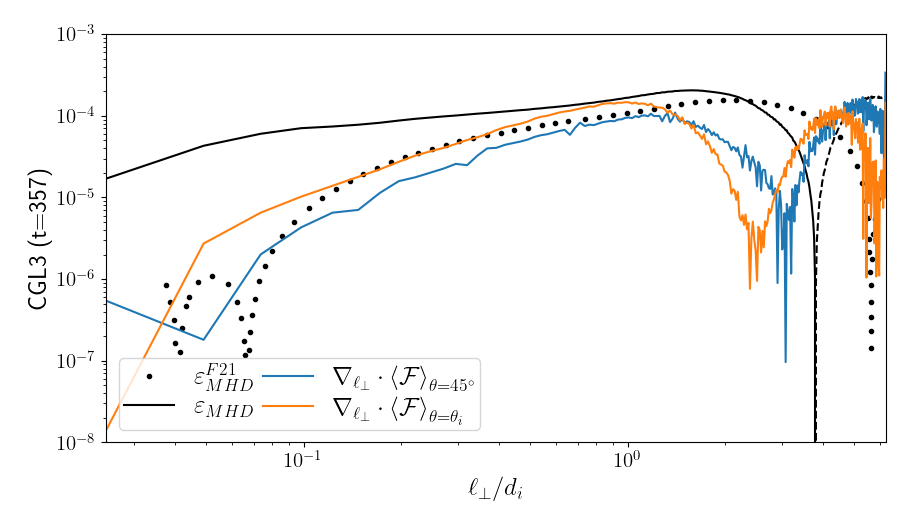
\includegraphics[width=0.9\linewidth,trim=0cm 0cm 0cm 0cm, clip=true]{./Mainmatter/Part_3/images_ch2/CGL3_compa_div}
 \cprotect\caption{Mode de représentation : \cacro{1D} en fonction de \ensuremath{\ell_{\perp}} normalisé par \ensuremath{d_i}. Simu : CGL3 (\ensuremath{t =\num{357}}). Comparaison de \ensuremath{\varepsilon_{MHD}} obtenu par \cacro{F21} (ligne noire pointillée), \cacro{FEL} (ligne noire pleine) et l'application d'une divergence transverse sur \ensuremath{\boldsymbol{\mathcal{F}}} calculés avec \cacro{FEL} et moyenné suivant deux angles \ensuremath{\theta = \ang{45}} de la boîte numérique et \ensuremath{\theta = \theta_i}. }
 \label{fig:compa_div}
 \end{figure} 
 
La \figref{fig:compa_div} illustre les effets de la variation parallèle de la composante parallèle du flux ainsi que ceux du filtrage. Le résultat \cacro{F21} (en pointillé) y est comparé à deux estimations de la divergence transverse effectuée dans nos résultats après avoir moyenné le flux dans le plan perpendiculaire et suivant les $\ell_{\parallel}$. On ne s'attend pas à retrouver exactement le résultat de \cacro{F21} mais à s'en rapprocher. La différence entre les deux estimations correspond au filtrage utilisé dans la moyenne de $\ell_{\parallel}$ : celui utilisé par \cacro{F21} en bleu, et celui que l'on utilise en orange. L'impact de l'angle de filtrage avait déjà été remarqué dans l'analyse de la \figref{fig:rep_CGL1}. On voit ici qu'il a pu influer sur le résultat de \cacro{F21} tout comme il peut influer sur le nôtre. On peut en déduire de cette figure que le poids des variations parallèles, omis par \cacro{F21}, semble avoir un impact sur nos résultats. 
 
 La différence entre nos estimations transverses et \cacro{F21} est située dans le nombre de points du maillage utilisé. Comme \cacro{FEL} prend en compte l'ensemble de l'espace des échelles, il donnera pour $\varepsilon_{MHD}$ par exemple, un résultat impacté par toutes ses variations spatiales omises par une moyenne sur un nombre réduit de vecteurs, malgré la compensation apportée par la pondération. Cet ensemble réduit d'échelles étant choisi tel des multiples de quelques vecteurs directionnels, il représentera d'autant moins les variations en s'approchant des grandes échelles.

 Il semble donc cohérent d'attribuer notre différence de comportement de $\varepsilon_{MHD}$ aux choix numériques façonnant le code de post-traitement. On peut aussi en déduire que \cacro{FEL} donne un résultat associé à la position dans l'espace \sacro{2D} plus réaliste que \cacro{F21}.
 
 \subsection{Effet du forçage sur la zone inertielle} \label{sec-322}
 
 La proximité du forçage induit de fortes variations dans le résultat à grande échelle. De plus, ici, cette injection est loin d'être stationnaire : parfois le forçage est allumé, d'autres fois, il est éteint. Sur la \figref{fig:compainc_t}, est affiché le résultat \cacro{IMHDH} pour différents temps de CGL3. 
 \begin{figure}[!ht]
  \centering
 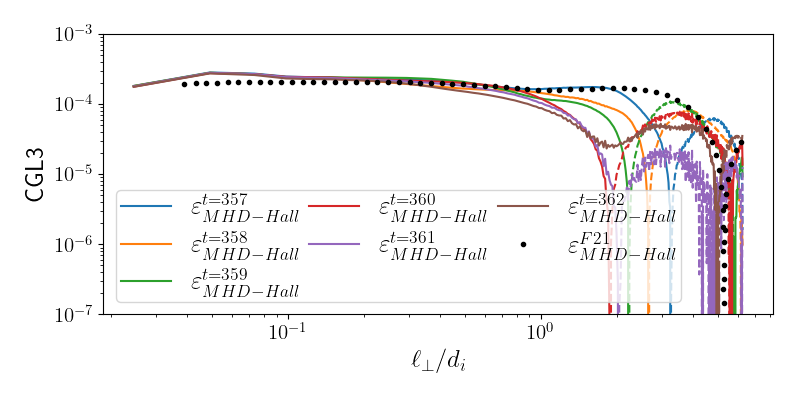
\includegraphics[width=0.9\linewidth,trim=0cm 0cm 0cm 0cm, clip=true]{./Mainmatter/Part_3/images_ch2/F19_time}
 \cprotect\caption{Mode de représentation : \cacro{1D} en fonction de \ensuremath{\ell_{\perp}} normalisé par \ensuremath{d_i}. \ensuremath{\varepsilon_{F19}} est obtenu pour divers temps \ensuremath{t} de CGL3, chaque temps correspond à une couleur. Le résultat extrait de la figure 5 de F21 est donné en pointillés noirs.}
 \label{fig:compainc_t}
 \end{figure} 
 On voit qu'en fonction du temps, l'échelle limite de la zone inertielle (telle que  $\varepsilon_{F19}$ constant) fluctue grandement. Et à $t=357$ (temps utilisé par \cacro{F21}), notre résultat (courbe bleue) montre la zone inertielle la plus large obtenue avec \cacro{FEL}. Le forçage est éteint de $t=357 $ à $t=360$ et la zone inertielle décroît petit à petit.  Puis, pour les temps suivant, il est rallumé et le plateau semble alors se reformer. On observe donc, ici, l'oscillation de l'injection. Aux échelles $\ell_{\perp}/d_i < 1$, le niveau de $\varepsilon_{F19}$ varie peu quel que soit le temps considéré. Cette observation concorde avec l'hypothèse de stationnarité statistique du taux de cascade dans la zone inertielle (ici \cacro{MHDH}). Cette hypothèse est considérée analytiquement pour obtenir des lois du type \cacro{K41} (voir synthèse \ref{synt-01}).  
 
 Le temps de simulation sélectionné impactant l'extension dans la zone de forçage de la zone inertielle, les temps de simulations indiqués dans la \tabref{tab:setups} ont été sélectionnés en prenant garde à l'état allumé ou éteint du forçage, mais cela ne signifie pas que l'extension de la zone inertielle se sera reformée. Une dernière différence, minime, n'a pas encore été abordée : celle de la variation aux petites échelles de $\varepsilon_{MHD-Hall}$. Sa signification associée à l'hyperdissipation sera abordée dans la section \ref{sec-323}.
 
 \section{Équation KHM et incertitude numérique} 
 \label{sec-323}
 
 Afin d'estimer l'incertitude sur nos résultats, nous nous sommes lancés dans la vérification de l'équation \cacro{KHM} du modèle simulé sous sa forme complète et pas seulement de la loi \cacro{K41} dont la validité est réduite à la zone inertielle. Cette estimation est permise par le travail analytique effectué en amont et décrit dans la Partie \ref{part_2}.
 
 \subsection{Calcul de la loi KHM}
 Une loi de type \cacro{KHM} peut s'écrire schématiquement (voir Chapitre \ref{ch-01}) : 
 \begin{equation}
  \label{eq:scheme_KHM_simu}   \partial_t \mathcal{R} =  \varepsilon_{NL} + \varepsilon_{D} + \varepsilon_{F}
 \end{equation}
 Nous avons vu que l'application des hypothèses de Kolmogorov donne la loi réduite de type \cacro{K41} $\varepsilon = - \varepsilon_{NL}$ (voir synthèse \ref{synt-01}). Son contenu, spécifique au modèle implémenté, sera détaillé dans les Chapitres \ref{ch-33} (\sacro{CGLHPe}) et \ref{ch-34} (\sacro{LFHPe}). 
 
 $ \partial_t \mathcal{R}$ est la dérivée temporelle de la fonction de corrélation utilisée pour obtenir la loi exacte. Dans nos études, cette fonction est  $ \mathcal{R} =\frac{1}{4} \left< (\rho'+\rho) (\boldsymbol{v'} \cdot  \boldsymbol{v} +  \boldsymbol{v'_A} \cdot  \boldsymbol{v_A}) + 2\rho' u + 2 \rho u'\right>$. Pour estimer ce terme, on va utiliser les temps consécutifs relevés dans la simulation. La dérivée temporelle sera estimée grâce à des schémas de discrétisation de type \og différences finies \fg{} d'ordre 2 : 
 \begin{itemize}
     \item décentrée vers la droite pour le premier temps $t_0$ : $ (\partial_t \mathcal{R})(t_0) = \frac{\mathcal{R}(t_0 + \delta t) - \mathcal{R}(t_0)}{\delta t}$,
     \item décentrée vers la gauche pour le dernier temps $t_{N_t}$ : $ (\partial_t \mathcal{R})(t_{N_t}) = \frac{\mathcal{R}(t_{N_t}) - \mathcal{R}(t_{N_t}-\delta t)}{\delta t}$,
     \item centrée pour les autres temps :  $ (\partial_t \mathcal{R})(t_n) = \frac{\mathcal{R}(t_{n+1}) - \mathcal{R}(t_{n-1}) }{2\delta t}$ avec $n\in ]0,N_t[$.
 \end{itemize}
 
  Le forçage présent dans nos simulations est un forçage de type antenne de Langevin appliqué sur le champ de vitesse. Par conséquent, le taux de forçage $\varepsilon_{F}$ s'écrira $\varepsilon_{F} = \frac{1}{4} \left< (\rho'+\rho) (\boldsymbol{v'} \cdot  \boldsymbol{f} + \boldsymbol{v} \cdot  \boldsymbol{f'} ) \right>$. Ce forçage dépend de deux composantes aléatoires qui font partie des quantités extraites de la simulation, elles seront notées $f_{sup}$ et $f_{inf}$. Elles permettent de construire une quantité intermédiaire $F = a_1 f_{sup} + (1-a_1) f_{inf}$ avec $a_1$ un paramètre égal à $0.5$ dans nos simulations. Les composantes de $\boldsymbol{f}$ sont alors : $f_x = \partial_y F$, $f_y = - \partial_x F$ et $f_z = 0$. 
  
  Enfin, le taux de dissipation $\varepsilon_{D}$ couvre l'ensemble des hyperdissipations présentes dans le système. Chaque quantité est associée à une hyperdissipation du type $ \nu_X \Delta^4 X$ avec $X$ quantité générique et $\Delta^4 = (\partial^2_x + \partial^2_y + \alpha \partial^2_z)^4$. On va décomposer $\varepsilon_{D}$ tel que : 
  \begin{equation}
      \varepsilon_{D} = \varepsilon^{c}_{D} + \varepsilon^{m}_{D} + \varepsilon^{ui}_{D} + \varepsilon^{ue}_{D}
  \end{equation}
  avec : 
  \begin{itemize}
      \item la contribution cinétique avec $\boldsymbol{D}_{\boldsymbol{v}} = \nu \Delta^4 \boldsymbol{v} $ et $D_{\rho} = \nu_{\rho} \Delta^4 \rho $ :
      \begin{equation}
          \varepsilon^{c}_{D} = \varepsilon^{c}_{D}(\boldsymbol{D_{v}}) + \varepsilon^{c}_{D}(D_{\rho})=   - \frac{1}{4} \left< \left(\rho'+\rho\right) \left(\boldsymbol{v'} \cdot  \boldsymbol{D_{\boldsymbol{v}}} + \boldsymbol{v} \cdot   \boldsymbol{D'_{\boldsymbol{v}}}  \right)\right>   - \frac{1}{4} \left<  \left(D'_{\rho}+D_{\rho}\right)  \boldsymbol{v'} \cdot  \boldsymbol{v}\right> 
      \end{equation}
      \item la contribution magnétique avec $\boldsymbol{D_{v_A}} = \frac{\eta}{\sqrt{\rho}} \Delta^4 (\sqrt{\rho} \boldsymbol{v_A})$ :
      \begin{eqnarray}
          \varepsilon^{m}_{D} = \varepsilon^{m}_{D}(\boldsymbol{D_{v_A}}) + \varepsilon^{m}_{D}(D_{\rho})&=& - \frac{1}{4} \left< \left(\rho'+\rho\right) \left(\boldsymbol{v'_A} \cdot  \boldsymbol{D_{v_A}} + \boldsymbol{v_A} \cdot   \boldsymbol{D'_{v_A}}  \right) \right>\nonumber \\
          &&- \frac{1}{8} \left<\left(\rho'-\rho\right) \left(\frac{D'_{\rho}}{\rho'}-\frac{D_{\rho}}{\rho}\right) \boldsymbol{v'_A} \cdot  \boldsymbol{v_A} \right>
      \end{eqnarray}  
      \item la contribution d'énergie interne ionique (gyrotrope) avec $D_u =  \frac{\nu_p}{2} \Delta^4 (2p_{\perp i } + p_{\parallel i })$ et sachant que $ \rho_i u_i = \frac{1}{2} (2 p_{\perp i } + p_{\parallel i })$:
      \begin{equation}
          \varepsilon^{ui}_{D} = \varepsilon^{ui}_{D}(D_u) + \varepsilon^{ui}_{D}(D_{\rho})=   - \frac{1}{2} \left<  \frac{\rho}{\rho'} D'_u +  \frac{\rho'}{\rho} D_u \right>- \frac{1}{2} \left< \left(\frac{ D'_{\rho}}{\rho'} - \frac{D_{\rho}}{\rho} \right)\left( \rho' u_i  -  \rho u'_i \right)   \right>  
      \end{equation}
      \item la contribution d'énergie interne électronique (isotherme) sachant que  $\rho_e u_e = \rho \ln \rho$ :
      \begin{equation}
          \varepsilon^{ue}_{D} =   - \frac{1}{2} \left<  D'_{\rho} \ln \rho +  D_{\rho} \ln \rho' +  \frac{\rho'}{\rho} D_{\rho} + \frac{\rho}{\rho'} D'_{\rho} \right>  
      \end{equation}
  \end{itemize}
 et $\nu$, $\eta$, $\nu_{\rho}$ et $\nu_p$ des constantes choisies empiriquement pour chaque simulation. Elles sont résumées dans la \tabref{tab:setups_hd}.
 
 %Sachant que dans la majorité des simulations du modèle MCGL, $\nu_{\rho} = 0$ et $\nu_p \ll \nu$, on a négligé les contributions d'énergie interne ainsi que les termes dépendant de $D_{\rho}$ dans les contributions cinétique et magnétique. 
 
 \subsection{Analyse des contributions de la loi KHM }
 
 Sur la \figref{fig:KHM}, $\varepsilon_{NL}$ (bleu) est comparé à un niveau de référence $\varepsilon_{ref} =- \partial_t \mathcal{R}  + \varepsilon_{D} + \varepsilon_{F}$ (violet), construit à partir de $\partial_t \mathcal{R}$ (rouge), $\varepsilon_{D}$ (vert) et $\varepsilon_{F}$ (orange). La différence $\zeta = \varepsilon_{ref} - \varepsilon_{NL}$ est donnée en marron. On remarque qu'elle n'est pas de l'ordre du zéro numérique ($\sim \num{e-20}$) mais environ deux ordres de grandeurs en dessous du niveau de $\varepsilon_{NL}$.  De plus, la forme des termes $\partial_t \mathcal{R}$, $\varepsilon_{D}$ et $\varepsilon_{F}$ est particulière.
 \begin{figure}[!ht]
  \centering
 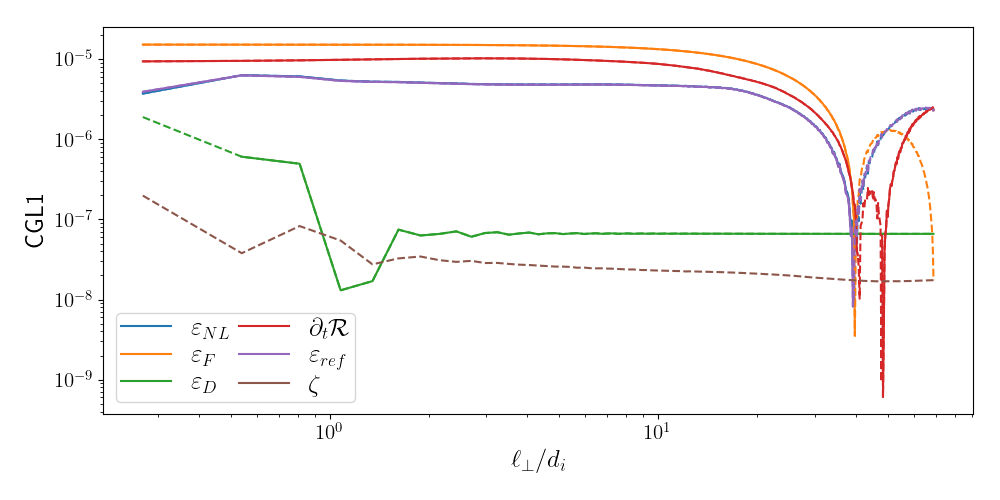
\includegraphics[width=0.9\linewidth,trim=0cm 0cm 0cm 0cm, clip=true]{./Mainmatter/Part_3/images_ch2/CGL1_1D_lperp_alll}
 %\hfill
 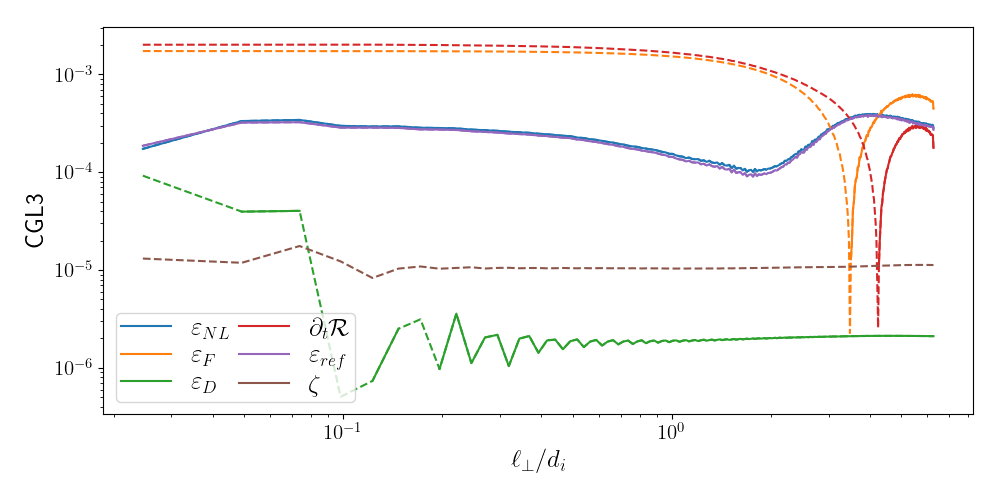
\includegraphics[width=0.9\linewidth,trim=0cm 0cm 0cm 0.5cm, clip=true]{./Mainmatter/Part_3/images_ch2/CGL3_1D_lperp_alll}
 \cprotect\caption{Détail de la loi \cacro{KHM} pour CGL1 (haut) et CGL3 (bas). Bleu : $\varepsilon_{NL}$. Orange : $\varepsilon_{F}$. Vert : $\varepsilon_{D}$. Rouge : $\partial_t \mathcal{R}$. Violet : $\varepsilon_{ref} =- \partial_t \mathcal{R}  + \varepsilon_{D} + \varepsilon_{F}$. Marron : $\zeta = \varepsilon_{ref} - \varepsilon_{NL}$. Représentation : \cacro{1D} en fonction de $\ell_{\perp}$ avec les valeurs positives en trait plein et négatives en trait discontinu. }
 \label{fig:KHM}
 \end{figure} 
 
 \paragraph{Balance des termes et forçage :  } 
 
 Tout d'abord, analysons la situation pour CGL1. Dans le Chapitre \ref{ch-01}, on a vu que : 
 \begin{equation}
     \label{eq:khm_a_verif} \varepsilon_{NL}(\boldsymbol{\ell})  = \varepsilon_{F}(\boldsymbol{\ell}) = \varepsilon_{D}(\boldsymbol{\ell} = 0) = - \varepsilon
 \end{equation}
  dans une zone inertielle où l'hypothèse de stationnarité statistique s'appliquerait. 
  
  On peut en effet identifier une gamme d'échelles $\ell_{\perp}/d_i \in \left[ \num{1}; \num{20}\right]$ telle que $\varepsilon_{NL}$ soit constant. Son niveau est alors d'environ $\num{5e-6}$. La valeur n'est pas visible ici à cause de l'échelle logarithmique mais $\varepsilon_{D}(\boldsymbol{\ell} = 0) \simeq \num{5e-6}$. Donc $\varepsilon_{NL}(\boldsymbol{\ell})  =  \varepsilon_{D}(\boldsymbol{\ell} = 0)$ semble retrouvé. Par contre, même si la constance\footnote{ Le comportement constant du terme de forçage est démontré rigoureusement dans l'annexe \ref{an:forc}.} de $\varepsilon_{F}$ est vérifiée à ces échelles, son niveau est beaucoup trop important, de l'ordre de $ \num{1.5e-5}$. Pour retrouver le niveau $\num{5e-6}$, on doit lui soustraire $\partial_t \mathcal{R}$ qui est d'environ $ \num{1e-5}$. La relation \eqref{eq:khm_a_verif} s'écrit alors dans nos simulations : 
  \begin{equation}
     \label{eq:khm_b_verif} \varepsilon_{NL}(\boldsymbol{\ell})  = \varepsilon_{F}(\boldsymbol{\ell}) - \partial_t \mathcal{R} = \varepsilon_{D}(\boldsymbol{\ell} = 0) = - \varepsilon
 \end{equation}
 
 \paragraph{Analyse du terme \ensuremath{\partial_t \mathcal{R}} :  } 
  Analytiquement, on se servait de l'hypothèse de stationnarité statistique pour annuler $\partial_t \mathcal{R}$, c'est-à-dire pour supposer qu'entre deux temps $\mathcal{R}$ ne varie pas. Puisque $\partial_t \left<E_{tot}\right>=\partial_t \mathcal{R}(\boldsymbol{\ell} = 0)$, si $\partial_t \mathcal{R}=0$ alors $\partial_t \left<E_{tot}\right>=0$.  Sauf que dans nos simulations $\left<E_{tot}\right>$ fluctue légèrement : pour les quatre temps consécutifs utilisés pour CGL1, $\left<E_{tot}\right>$, de l'ordre de $\num{1.3e0}$, augmente d'environ $\num{6e-7}$ par pas de temps. Par conséquent, $\partial_t \mathcal{R}=0$ est impossible à obtenir. C'est ce que l'on observe sur la \figref{fig:KHM} pour CGL1 comme pour CGL3. Pourtant, la convergence temporelle des résultats du calcul de loi exacte \cacro{K41} dans une certaine zone d'échelles a bel et bien été observée sur la \figref{fig:compainc_t}, et cela nous semblait une belle preuve de la stationnarité statistique de nos simulations. À première vue, ces résultats ne semblent pas compatibles. L'interprétation de ce paradoxe reste à affiner mais le comportement du $\partial_t \mathcal{R}$ instantané tel un forçage ne semble pas être une spécificité de nos simulations. En effet, \cite{ferrand_-depth_2022} trouvent un comportement similaire dans des simulations de turbulence non forcée, pour lesquelles l'énergie totale moyenne est en  décroissance perpétuelle. Dans notre cas, on pourrait peut-être interpréter le comportement du terme $\partial_t \mathcal{R}$ comme un réservoir d'énergie régulant temporellement l'injection de l'énergie dans la cascade afin que cette dernière puisse s'effectuer au taux imposé par les processus de dissipation. 
 
  \paragraph{Analyse des contributions d'hyperdissipation :  } 
  
   Un autre comportement pathologique est celui de $\varepsilon_{D}$ en fonction de $\ell$. Dans la théorie analytique, ce terme est supposé nul à toutes les échelles sauf en $\ell = 0$ à cause de l'anomalie dissipative. Dans nos simulations, son rôle est joué par les termes d'hyperdissipation, mais on s'attendrait à ce qu'ils décroissent rapidement en allant vers les grandes échelles puisque la dérivation par $\Delta^4$ impose un comportement en $k^8$ dans l'espace de Fourier. Regardons ce qu'il en est en le décomposant sur ses diverses contributions. La décomposition est présentée sur la \figref{fig:DISS}. 
 \begin{figure}[!ht]
  \centering
 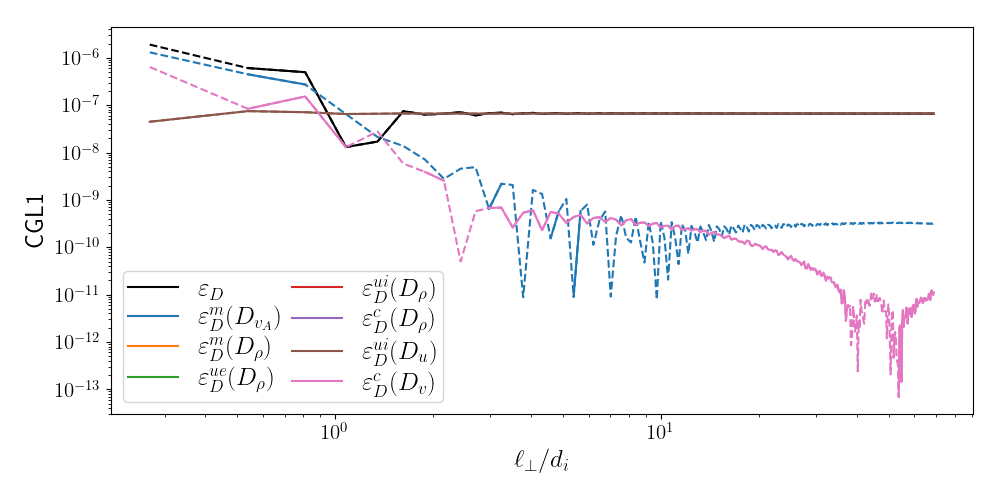
\includegraphics[width=0.9\linewidth,trim=0cm 0cm 0cm 0cm, clip=true]{./Mainmatter/Part_3/images_ch2/CGL1_1D_lperp_dissl}
 %\hfill
 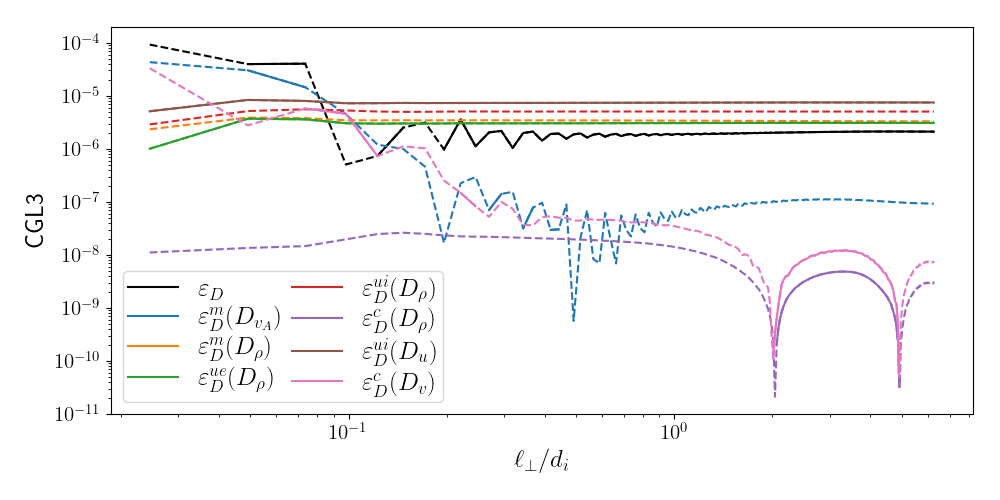
\includegraphics[width=0.9\linewidth,trim=0cm 0cm 0cm 0.5cm, clip=true]{./Mainmatter/Part_3/images_ch2/CGL3_1D_lperp_dissl}
 \cprotect\caption{Détail du terme d'hyperdissipation, $\varepsilon_{D}$ (noir), pour CGL1 (haut) et CGL3 (bas). Bleu : $\varepsilon^m_{D}(D_{\boldsymbol{v_A}})$. Orange :  $\varepsilon^m_{D}(D_{\rho})$. Vert :  $\varepsilon^{ue}_{D}(D_{\rho})$. Rouge : $\varepsilon^{ui}_{D}(D_{\rho})$. Violet :  $\varepsilon^c_{D}(D_{\rho})$ Marron :  $\varepsilon^{ui}_{D}(D_{u})$. Rose :  $\varepsilon^c_{D}(D_{v})$. Représentation : \cacro{1D} en fonction de $\ell_{\perp}$ avec les valeurs positives en trait plein et négatives en trait discontinu.}
 \label{fig:DISS}
 \end{figure}
 On y voit que chacune des contributions semble ou décroître en allant vers les grandes échelles ou rester constante. Les termes en $D_{\rho}$ (visibles seulement pour CGL3 puisque $\nu_{\rho} = 0$ pour CGL1) et $D_u$ ne montrent pas de décroissance, et la tendance en environ $\ell^{-2}$ de la décroissance de $\varepsilon^{c}_{D}(\boldsymbol{D_{v}})$ et $\varepsilon^{m}_{D}(\boldsymbol{D_{v_A}})$ avait été remarquée par \cite{ferrand_multi-scale_2021} dans le cas incompressible. La pathologie de cette pente en $-2$ y avait été identifiée et associée à une saturation mathématique de la fonction de corrélation calculée entre deux points. Cette saturation est due à une puissance de $k$ trop importante dans l'espace de Fourier et est similaire à celle relevée par \cite{cho_simulations_2009}. 
 
 Dans l'Annexe \ref{an:sat}, nous proposons une démonstration mathématique de ce phénomène en fonction du type de la fonction de corrélation, incrémentale ou non, et de la tendance du spectre dans l'espace de Fourier. On y obtient dans le cas non incrémental, pour la corrélation de deux quantités indéfinies $A$ et $B$, : 
 \begin{eqnarray}
   \label{eq:sat_noninc}  \left<A({\bf x} + \boldsymbol{\ell})  \cdot B({\bf x}) + A({\bf x})  \cdot B({\bf x} + \boldsymbol{\ell})\right> 
 \propto \left\{
     \begin{aligned}
     &\ell^{-2}& \textrm{si $m \in ]-\infty,-1[$ } \\
  &\ell^{m-1}&  \textrm{si $m \in ]-1,1[$}  \\
  &1& \textrm{si $m \in ]1,+\infty[$ } 
 \end{aligned}
 \right.%\nonumber  \\
 \end{eqnarray}
 avec $m$, la pente du spectre unidimensionnel en représentation logarithmique tel que $k^{-m}$. 
 
 Pour une fonction de corrélation incrémentale on obtient :
 \begin{eqnarray}
    \label{eq:sat_inc} \left<(A({\bf x} + \boldsymbol{\ell}) - A({\bf x}))\cdot(B({\bf x} + \boldsymbol{\ell}) - B({\bf x})) \right> 
 \propto \left\{
     \begin{aligned}
     & 1 & \textrm{si $m \in ]-\infty,1[$ } \\
 & \ell^{m-1}&  \textrm{si $m \in ]1,3[$ }  \\
 & \ell^2 & \textrm{si $m \in ]3,+\infty[$}
 \end{aligned}
 \right. .%\nonumber\\
 \end{eqnarray}
 Si l'on analyse les différentes contributions du terme de dissipation, on se rend compte que $ \varepsilon^{c}_{D}(\boldsymbol{D_{v}}) $, $ \varepsilon^{c}_{D}(D_{\rho})$, $\varepsilon^{m}_{D}(\boldsymbol{D_{v_A}}) $,
 $ \varepsilon^{ui}_{D}(D_u) $ et $\varepsilon^{ue}_{D}$ ont une forme assez proche d'une fonction de corrélation non incrémentale et $ \varepsilon^{m}_{D}(D_{\rho}) $ tandis que  $\varepsilon^{ui}_{D}(D_{\rho})$ sont plus proches d'une fonction incrémentale. 
 
 Pour une pente de spectre autour de $k^8$ ($m=-8$), une fonction de corrélation non incrémentale va saturer en $\ell^{-2}$. On retrouve ce comportement pour $ \varepsilon^{c}_{D}(\boldsymbol{D_{v}}) $ et  $\varepsilon^{m}_{D}(\boldsymbol{D_{v_A}}) $. Tandis qu'une fonction de corrélation incrémentale va saturer en $\ell^0$ (comportement retrouvé pour  $ \varepsilon^{m}_{D}(D_{\rho}) $ et  $\varepsilon^{ui}_{D}(D_{\rho})$). On retrouve aussi le comportement du terme de forçage (fonction de corrélation non incrémentale) constant loin des échelles de forçage, puisqu'un Dirac à petit $\ell$ peut-être vu comme une pente en $m = +\infty$. Ces comportements plus mathématiques que physiques sont retrouvés pour toutes les simulations. 
 
 On remarque tout de même les fortes variations des termes décroissant en $\ell^{-2}$. Ces variations sont la cause de la bosse visible aux plus petites échelles pour tous les taux $\varepsilon_{NL}$ et $\varepsilon$ calculés dans les simulations et que l'on avait remarquée dans la section \ref{sec-321}. En effet, $\varepsilon_F - \partial_t \mathcal{R} $ reste constant dans cette zone alors que la bosse apparaît dans $\varepsilon_F - \partial_t \mathcal{R} + \varepsilon_D $. Cette bosse nous indique donc les échelles auxquelles l'erreur mathématique de l'hyperdissipation impacte systématiquement $\varepsilon_{NL}$ et ses contributions.  
 
  Ce type d'erreur mathématique pourrait aussi impacter $\partial_t \mathcal{R}$, $\mathcal{R}$ étant une fonction de corrélation en deux points.
  
  \subsection{Estimation de l'erreur sur le taux de cascade  } 
 
 Les fonctions de corrélation en deux points ne sont donc pas adaptées à l'étude de la physique des termes d'hyperdissipation et de ceux inclus dans $\partial_t \mathcal{R}$ comme a pu le faire remarquer \cite{cho_simulations_2009}\footnote{La solution proposée par \cite{cho_simulations_2009} est d'augmenter le nombre de points servant au calcul de la fonction de corrélation. Une telle tâche s'annonce mathématiquement complexe et lourde dans le cadre de la théorie des lois exactes. Une autre possibilité est d'estimer précisément pour chaque contribution la puissance $m$ du spectre influant sur le résultat de chaque contribution au taux de dissipation, puis de calculer la tendance attendue en $\ell^{m-1}$ [\cite{ferrand_multi-scale_2021}].}. Par la suite, nous nous concentrerons seulement sur $\varepsilon_{NL}$ et ses contributions, mais nous garderons en mémoire les influences potentielles de ces termes.
 
 L'analyse des différentes contributions à la loi \cacro{KHM} permet ainsi d'identifier les sources d'erreurs numériques et mathématiques menant au niveau de $\zeta$. Ce dernier, de l'ordre des fluctuations de $\left< E_{tot}\right>$, reflèterait la signature de la quasi-stationnarité statistique des simulations. Aux échelles plus faibles, la saturation mathématique du calcul des fonctions de corrélation dépendant de l'hyperdissipation ainsi que sa signature\footnote{Les corrélations impliquées dans $\varepsilon_{D}$ étant d'ordre 2 et celles présentes dans les termes dominant de $\varepsilon_{NL}$ étant d'ordre 3, le reflet dans $\varepsilon_{NL}$ de l'erreur mathématique pourrait, à priori, ne pas compenser exactement l'erreur sur $\varepsilon_{D}$. } dans $\varepsilon_{NL}$ semblent impacter $\zeta$. Ce dernier correspond donc à l'incertitude systématique de notre estimation du taux de cascade, incertitude provenant des données initiales, de leur adéquation avec les hypothèses de Kolmogorov et du schéma numérique utilisé pour le calcul des termes des lois exactes. Par la suite, les contributions qui apparaîtront inférieures à $\zeta$ seront alors supposés dans la zone d'incertitude du taux de cascade total. Leur analyse devra donc être effectuée avec précautions. 
 
 Un autre point reste à éclaircir dans cette étude sur les lois du type \cacro{KHM} : la différence entre la loi obtenue en utilisant $\mathcal{R}$ et celle en utilisant une fonction incrémentale $\mathcal{S}$. La fonction $\mathcal{S}$ associée à $\mathcal{R}$ est :
 \begin{equation}
    \label{eq:scheme_khms} \mathcal{S} = \frac{1}{4} \left< \delta (\rho \boldsymbol{v}) \cdot \delta \boldsymbol{v} + \delta (\rho \boldsymbol{v_A}) \cdot \delta \boldsymbol{v_A}  + 2 \delta \rho \delta u \right>
 \end{equation}
 On a alors la relation $\mathcal{S} = \left<E_{tot}\right> - \mathcal{R}$. Sachant que $\mathcal{R}(\boldsymbol{\ell} = 0) = \left<E_{tot}\right>$, il est facile de passer de l'expression \eqref{eq:scheme_KHM_simu} à la loi :
 \begin{equation}
  \label{eq:scheme_KHMS_simu}   \partial_t \mathcal{S} = - \mathcal{E}_{NL} + \mathcal{E}_{D} + \mathcal{E}_{F}
 \end{equation}
 avec $\mathcal{E}_{NL} = \varepsilon_{NL}(\boldsymbol{\ell} = 0) - \varepsilon_{NL}$, $\mathcal{E}_{D} = \varepsilon_{D}(\boldsymbol{\ell} = 0) - \varepsilon_{D}$ et $\mathcal{E}_{F} = \varepsilon_{F}(\boldsymbol{\ell} = 0) - \varepsilon_{F}$. 
 
 \begin{figure}[!ht]
  \centering
 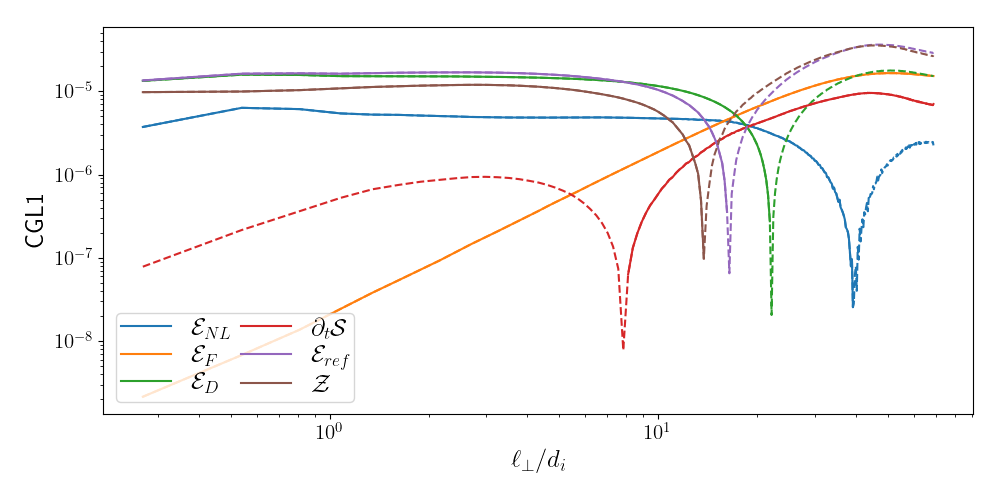
\includegraphics[width=0.9\linewidth,trim=0cm 0cm 0cm 0cm, clip=true]{./Mainmatter/Part_3/images_ch2/CGL1_1D_lperp_allSl}
 %\hfill
 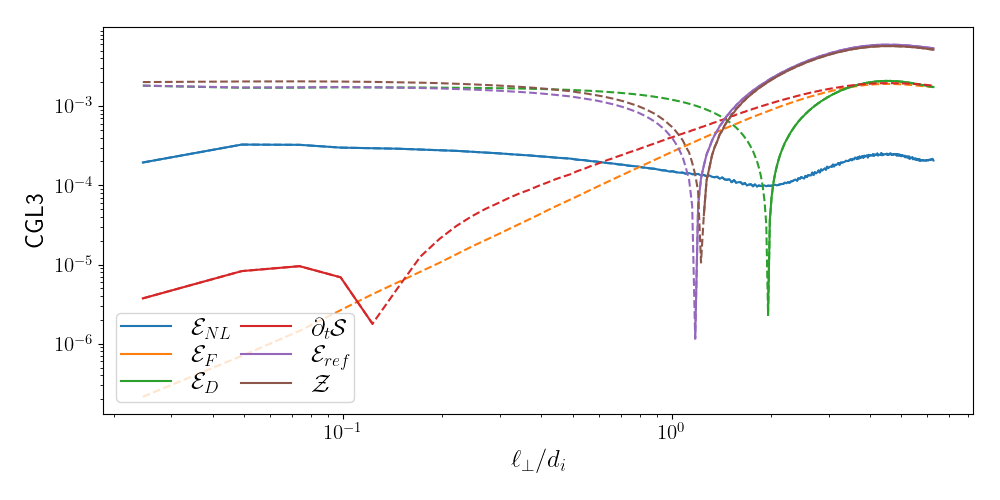
\includegraphics[width=0.9\linewidth,trim=0cm 0cm 0cm 0.5cm, clip=true]{./Mainmatter/Part_3/images_ch2/CGL3_1D_lperp_allSl}
 \cprotect\caption{Détail de la loi \eqref{eq:scheme_khms} pour CGL1 (haut) et CGL3 (bas). Bleu : \ensuremath{\mathcal{E}_{NL}}. Orange : \ensuremath{\mathcal{E}_{F}}. Vert : \ensuremath{\mathcal{E}_{D}}. Rouge : \ensuremath{\partial_t \mathcal{S}}. Violet : \ensuremath{\mathcal{E}_{ref} =- \partial_t \mathcal{S}  + \mathcal{E}_{D} + \mathcal{E}_{F}}. Marron : \ensuremath{\mathcal{Z} = \mathcal{E}_{ref} - \mathcal{E}_{NL}}. Représentation : \cacro{1D} en fonction de \ensuremath{\ell_{\perp}} avec les valeurs positives en ligne pleine et négatives en ligne dicontinue. }
 \label{fig:KHMS}
 \end{figure}
 
On notera que l'équation d'énergie totale s'écrit sous la forme $\partial_t E_{tot} + \nabla \cdot \boldsymbol{F_{tot}} = S$ avec $S$ les termes sources (dissipation et forçage), et $\boldsymbol{F_{tot}}$ le total de flux. De plus, puisque $\left<  \nabla \cdot \boldsymbol{F_{tot}} \right> = \nabla_{\boldsymbol{\ell}} \cdot \left< \boldsymbol{F_{tot}} \right> = - \left<  \nabla' \cdot \boldsymbol{F_{tot}} \right> = 0$, alors $\mathcal{E}_{NL} =  - \varepsilon_{NL}$.
 
 
 En appliquant cette transformation sur le détail de la loi \cacro{KHM} (\figref{fig:KHM}), on obtient les résultats de la  \figref{fig:KHMS}. On y remarque que le comportement des termes de forçage (orange) et de dissipation (vert) se sont inversés. $\mathcal{E}_{F}$ augmente en allant des petites vers les grandes échelles, avec une pente de facteur $2$, et $\mathcal{E}_{D} $ reste constant avant de changer de signe vers les grandes échelles. Ces comportements sont cohérents avec ceux démontrés dans les Annexes \ref{an:forc} et \ref{an:sat} (voir équations \eqref{eq:sat_noninc} et \eqref{eq:sat_inc}). Par contre, la différence $ \mathcal{Z} = \mathcal{E}_{ref} - \mathcal{E}_{NL} = (- \partial_t \mathcal{S} + \mathcal{E}_{D} + \mathcal{E}_{F}) - \mathcal{E}_{NL}$ est supérieure à $\zeta$. L'utilisation d'une fonction de corrélation incrémentale dans une étude de données de simulations semble donc amplifier l'erreur numérique et mathématique associée aux termes temporels, de dissipation et de forçage en y ajoutant l'erreur sur l'équation de $\left<E_{tot}\right>$. 
 
 %\newpage
 \section{Synthèse des tests de validation et sources d'erreurs }
 \label{synt-32}
 \fcolorbox{red}{white}{\begin{minipage}[c]{\linewidth}
 Ces études sont illustrées par les résultats obtenus pour les simulations CGL1 et CGL3. 
 
 \paragraph{Comparaison Inc-MHD-Hall avec les résultats de \cite{ferrand_multi-scale_2021} :}
 \begin{itemize}
     \item le comportement des lois \cacro{IMHDH} est retrouvé,
     \item effets de nos choix de schéma numérique. 
 \end{itemize}
 
 \paragraph{Effet du forçage sur la zone inertielle visualisée avec Inc-MHD-Hall :}
 \begin{itemize}
     \item visualisation des oscillations induites par l'injection d'energie dans le taux de cascade : extension/réduction de la zone inertielle sur environ une demi décade,
     \item visualisation de l'impact de la stationnarité statistique : amortissement des oscillations et convergence de la zone inertielle.
 \end{itemize}
 
 % \paragraph{Comparaison MHD incompressible avec la formulation de PP98 donnée par \cite{banerjee_alternative_2017} : }
 % \begin{itemize}
 %     \item comportement global retrouvé
 %     \item  différences induites par la quasi-incompressibilité des simulations
 % \end{itemize}
 
 % \paragraph{Comparaison MHD compressible avec pression isotrope avec les prédictions de \cite{andres_energy_2018} : }
 % \begin{itemize}
 %     \item  formulation f1 cohérente avec les prédictions
 %     \item validation de l'apport de f2 sur f1 et cohérence avec les prédictions
 % \end{itemize}
 
 \paragraph{Analyse de la loi KHM : }
 \begin{itemize}
     \item paradoxe sur l'hypothèse de stationnarité statistique dans les simulations,
     \item saturation mathématique apportée par l'hyperdissipation,
     \item incertitude provenant de l'utilisation de fonctions incrémentales,
     \item estimation de l'erreur numérique et mathématique sur la loi exacte totale associée au modèle simulé, noté $\zeta$. \\
 \end{itemize}
 
 {\bf Ces études valident le schéma numérique et son implémentation, et questionnent les comportements non-physiques pouvant impacter les résultats.} \\
 
 Les Annexes \ref{an:A} et \ref{an:B} contiennent des études complémentaires pour ce chapitre.
 \end{minipage}}

 Dans ce chapitre, nous attaquons le cœur de l'étude numérique dont l'objectif est de répondre à la question : quel est l'impact de la correction dépendant de l'anisotropie de pression sur le taux de cascade ? Les résultats montrés ici sont récents, préliminaires et leur interprétation est encore en cours de discussion.
 
 \section{Le modèle CGL simulé} \label{sec-331}
 
 Dans un premier lot de simulations, les ions sont décrits avec la fermeture \cacro{CGL} et les électrons avec une fermeture isotherme qui correspond à notre fermeture isotherme-isentrope. La contribution des flux de chaleur est supposée nulle. La pression électronique est définie telle que $p_e = \rho$. Le modèle général \sacro{CGLHPe} simulé dans le code versatile est donné dans la section \ref{sec-233}. Regardons à quoi il ressemble si l'on y injecte les fermetures et que l'on y applique la normalisation indiquée dans la section \ref{sec-311} et utilisée dans l'implémentation des équations. Les équations de ce modèle sont ainsi :
 \begin{eqnarray}
 \label{eq:mcgl_r} \partial_t \rho + \nabla \cdot \left(\rho \boldsymbol{v}\right) &=& 0,\\
 \label{eq:mcgl_v} \partial_t  \boldsymbol{v} + \boldsymbol{v} \cdot \nabla  \boldsymbol{v} - \frac{1}{\rho} \boldsymbol{j} \times \boldsymbol{B} + \frac{1}{\rho} \nabla \cdot \overline{\boldsymbol{P}}  &=& 0,  \\
 \label{eq:mcgl_b} \partial_t \boldsymbol{B} - \nabla \times \left( \boldsymbol{v} \times \boldsymbol{B} \right) +  d_i  \nabla \times \left( \frac{1}{\rho} \boldsymbol{j}\times \boldsymbol{B} \right) &=& 0 , \\
 \label{eq:mcgl_pperp} \partial_t  p_{\perp i }  +  \nabla \cdot \left(p_{\perp i } \boldsymbol{v} \right) +  p_{\perp i }\nabla \cdot\boldsymbol{v} -  p_{\perp i } \boldsymbol{b}\boldsymbol{b} : \nabla \boldsymbol{v}  &=& 0  ,\\
 \label{eq:mcgl_ppar} \partial_t  p_{\parallel i }  +  \nabla \cdot \left(p_{\parallel i } \boldsymbol{v} \right) +  2 p_{\parallel i }  \boldsymbol{b}\boldsymbol{b} : \nabla \boldsymbol{v}  &=& 0  ,
 \end{eqnarray}
 en notant $\overline{\boldsymbol{P}} =  \frac{\beta_0}{2} \left(\overline{\boldsymbol{P_i}} + \rho \overline{\boldsymbol{I}} \right)$ avec $\overline{\boldsymbol{P_i}} = p_{\perp i } \overline{\boldsymbol{I}} + \left(p_{\parallel i } - p_{\perp i }\right) \boldsymbol{b} \boldsymbol{b}$ le tenseur gyrotrope de pression ionique, $\boldsymbol{b} = \frac{\boldsymbol{B}}{|\boldsymbol{B}|}$ la direction du champ magnétique et $\frac{\beta_0}{2} $ une constante provenant de la normalisation des équations.
 
 L'hypothèse isotherme vient annuler la contribution $\nabla P_e$ présente dans l'équation d'induction \eqref{eq:model_simu_b} puisque : 
 \begin{equation*}
      \nabla \times \left( \frac{1}{\rho} \nabla \left(  p_e\right) \right) =  \nabla \times \left( \frac{1}{\rho} \nabla  \rho \right) = \nabla \times  \nabla \left( \ln \rho \right) = 0.
 \end{equation*}
 On s'attend donc à ce que la contribution de $\nabla P_e$ permettant de compenser l'effet de ce terme dans l'équation d'énergie totale s'annule aussi. L'énergie interne étant $\rho u = \frac{\beta_0}{2} \left(p_{\perp i } + \frac{1}{2}p_{\parallel i} + \rho \ln \rho \right) $, son équation peut en effet s'écrire :
 \begin{eqnarray}
 \label{eq:mcgl_ui} \partial_t \left(\rho u\right) + \nabla \cdot \left(\rho u \boldsymbol{v}\right) +  \overline{\boldsymbol{P}}: \nabla \boldsymbol{v} &=& 0.
 \end{eqnarray}
 
 On reconnaît dans ces équations le modèle ayant donné la loi exacte \eqref{eq:turb_cpg_elk} ainsi que le terme de \cacro{Hall} dans l'équation \eqref{eq:mcgl_b} qui indique qu'il faut prendre en compte la correction \cacro{Hall} donnée par \eqref{eq:corr_hall}. Le taux de transfert non linéaire $\varepsilon_{NL}$ obtenu, qui est aussi valable en dehors de la zone inertielle, sera noté $\varepsilon_{cgl}$. On le comparera à $\varepsilon_{iso}$ calculé avec la partie isotrope du tenseur de pression\footnote{Le comportement de $\varepsilon_{iso}$ est connu, il a été étudié par \cite{andres_energy_2018} dans le cas isotherme. Comme nous utilisons une nouvelle formulation de la loi exacte, une vérification des prédictions est détaillée dans l'Annexe \ref{an:compa_predict}.}. On s'attend, pour ces quantités, à observer une zone inertielle élargie de la zone \cacro{MHD} à la zone \cacro{Hall}. 
 La différence $\varepsilon_{\overline{\boldsymbol{\Pi}}}=\varepsilon_{cgl}-\varepsilon_{iso}$ correspond à la contribution de l'anisotropie de pression donnée par l'équation \eqref{eq:turb_cpgyr_an}. Elle sera décomposée en quatre termes : 
 \begin{itemize}
     \item un terme flux : $\nabla_{\boldsymbol{\ell}} \cdot \boldsymbol{\mathcal{F}_A} = \frac{1}{4} \nabla_{\boldsymbol{\ell}} \cdot \left< \delta \rho \delta \left(\frac{\overline{\boldsymbol{\Pi}}}{\rho}\right) \cdot \delta \boldsymbol{v} \right> $,
     \item le terme source survivant dans la limite incompressible : 
     \begin{equation*}
         \mathcal{S}_{A1} = \frac{1}{2}\left<  \delta \left(\frac{\overline{\boldsymbol{\Pi}}}{\rho}\right) : \left(\rho\nabla' \boldsymbol{v'} -  \rho'\nabla  \boldsymbol{v}\right)\right>,
     \end{equation*}
     \item le terme source compressible dépendant explicitement des fluctuations de pression : 
     \begin{equation*}
         \mathcal{S}_{A2} =  \frac{1}{4}  \left<\delta \left(\frac{\overline{\boldsymbol{\Pi}}}{\rho}\right) : \left(\rho \boldsymbol{v} \frac{\nabla' \rho'}{\rho'} -\rho'\boldsymbol{v'}  \frac{\nabla \rho}{\rho} \right)  \right>,
     \end{equation*}
     \item le terme source dépendant explicitement des fluctuations de densité : 
     \begin{equation*}
         \mathcal{S}_{A3} = - \frac{1}{4}\left< \delta \rho \left(  \boldsymbol{v} \cdot   \left(\frac{\overline{\boldsymbol{\Pi}}}{\rho}\right) \cdot  \frac{\nabla' \rho'}{\rho'} - \boldsymbol{v'} \cdot \left(\frac{\overline{\boldsymbol{\Pi'}}}{\rho'}\right) \cdot  \frac{\nabla \rho}{\rho}\right) \right>,
     \end{equation*}
 \end{itemize}
 avec $\overline{\boldsymbol{\Pi}} =  \frac{\beta_0}{2} \left(p_{\parallel i } - p_{\perp i }\right)\left( \boldsymbol{b} \boldsymbol{b} - \frac{1}{3}  \overline{\boldsymbol{I}} \right)$. Cette contribution anisotrope est entièrement portée par les ions.
 
 \section{Étude de la loi CGL-MHD-Hall-\ensuremath{\nabla P_e} dans les simulations CGL1, CGL2, CGL3}
 \label{sec-332} 
 
 Tout d'abord, nous avons entrepris l'analyse des simulations CGL1, CGL2 et CGL3.
 Ce sont les simulations \sacro{CGLHPe} analysées dans l'article de \cite{ferrand_fluid_2021}, leurs paramètres sont résumés dans la \tabref{tab:setups} et la \tabref{tab:setups_hd}. Ces trois simulations sont initialisées telles que $a_{pi} = 1$. 
 
 \subsection{Loi globale et contribution de l'anisotropie de pression}
 La \figref{fig:trip_CGL1-2} (CGL1 et CGL2) et la \figref{fig:trip_CGL3} (CGL3) contiennent des triptyques associés à chaque simulation et permettant de comparer les taux de cascade $\varepsilon_{iso} $ et  $\varepsilon_{cgl}$. La différence des deux $\varepsilon_{\overline{\boldsymbol{\Pi}}} $ est représentée en \sacro{2D} en fonction de $\ell_{\perp}$ et $\ell_{\parallel}$, et est projetée dans les représentations \cacro{1D} sous la forme de courbe verte. Sur les représentations \cacro{1D}, sont ajoutés $\varepsilon_{cgl}$ en bleu, $\varepsilon_{iso}$ en orange et le niveau d'incertitude $\zeta$ en gris qui reste assez éloigné des autres quantités.
 
 \begin{figure}[!ht]
  \centering
  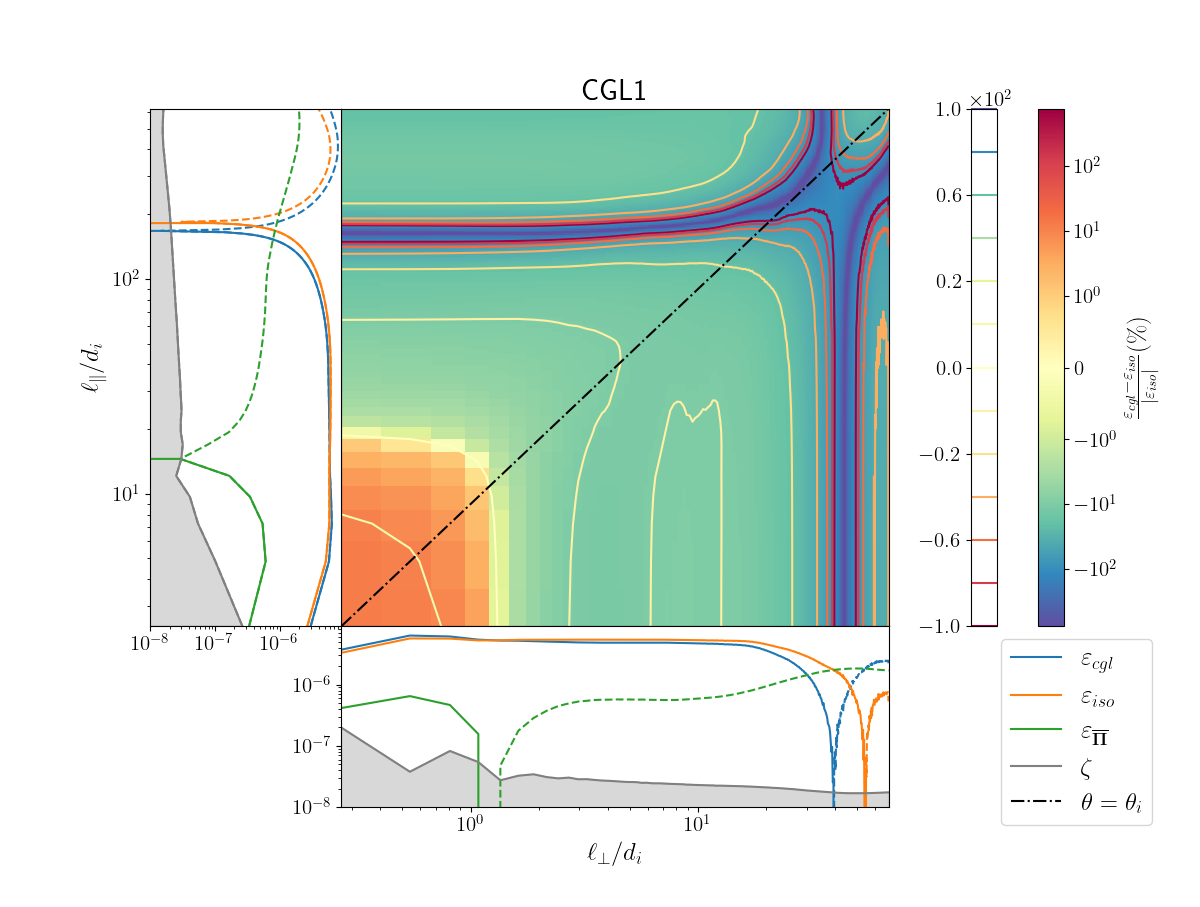
\includegraphics[width=0.95\linewidth,trim=1cm 0cm 0cm 2cm, clip=true]{./Mainmatter/Part_3/images_ch3/CGL1_panel_isocgl_percent}
 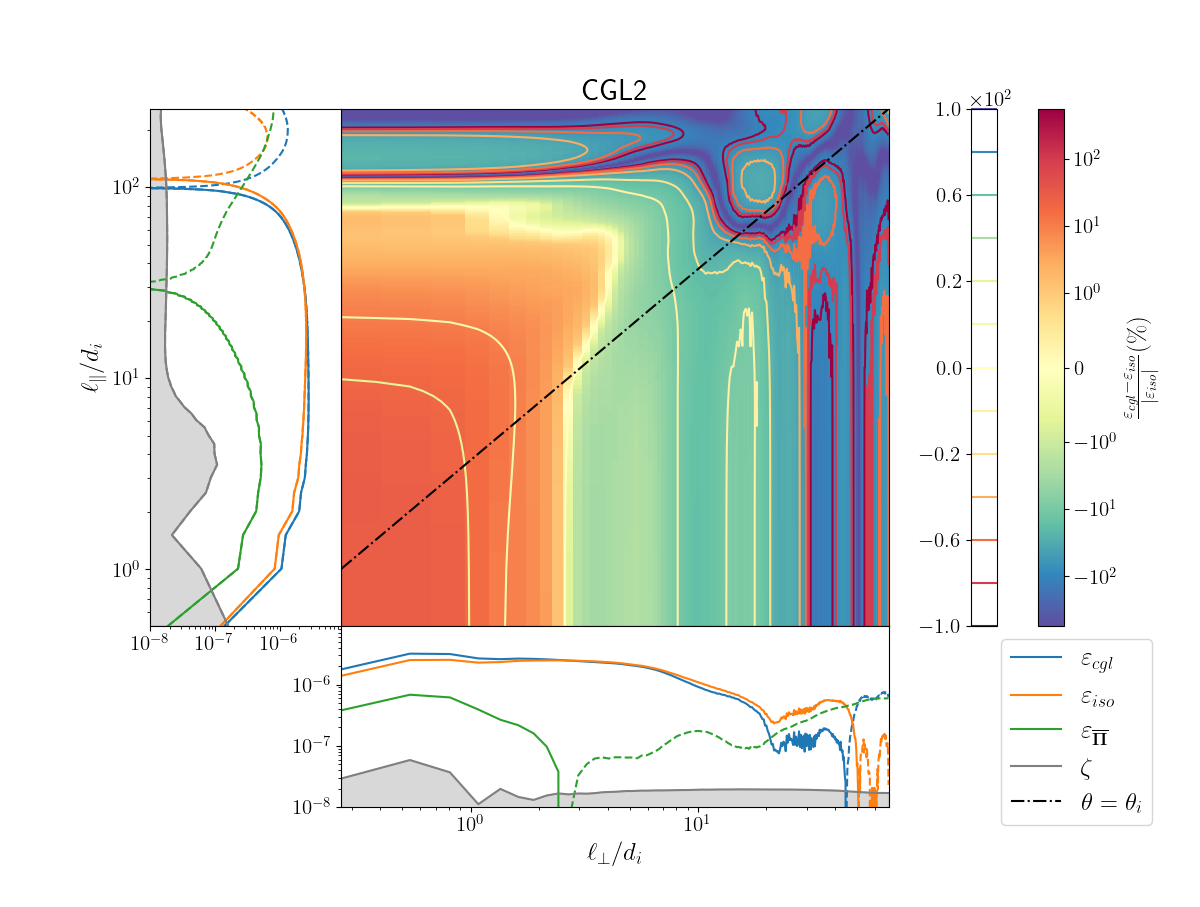
\includegraphics[width=0.95\linewidth,trim=1cm 0cm 0cm 2cm, clip=true]{./Mainmatter/Part_3/images_ch3/CGL2_panel_isocgl_percent}
 \cprotect\caption{Simu : CGL1 et CGL2. Représentation \cacro{2D} en fonction de \ensuremath{\ell_{\perp}} et \ensuremath{\ell_{\parallel}} de \ensuremath{\varepsilon_{cgl}-\varepsilon_{iso}} par rapport à \ensuremath{|\varepsilon_{iso}|} en \ensuremath{\%}, entourée des représentations \cacro{1D} en fonction de \ensuremath{\ell_{\perp}} (bas) et \ensuremath{\ell_{\parallel}} (gauche) de \ensuremath{\varepsilon_{iso}} (orange), \ensuremath{\varepsilon_{cgl}} (bleu), \ensuremath{\varepsilon_{\overline{\boldsymbol{\Pi}}}} (vert) et \ensuremath{\zeta} (gris). }
 \label{fig:trip_CGL1-2}
 \end{figure}
 \begin{figure}[!ht]
  \centering
 % 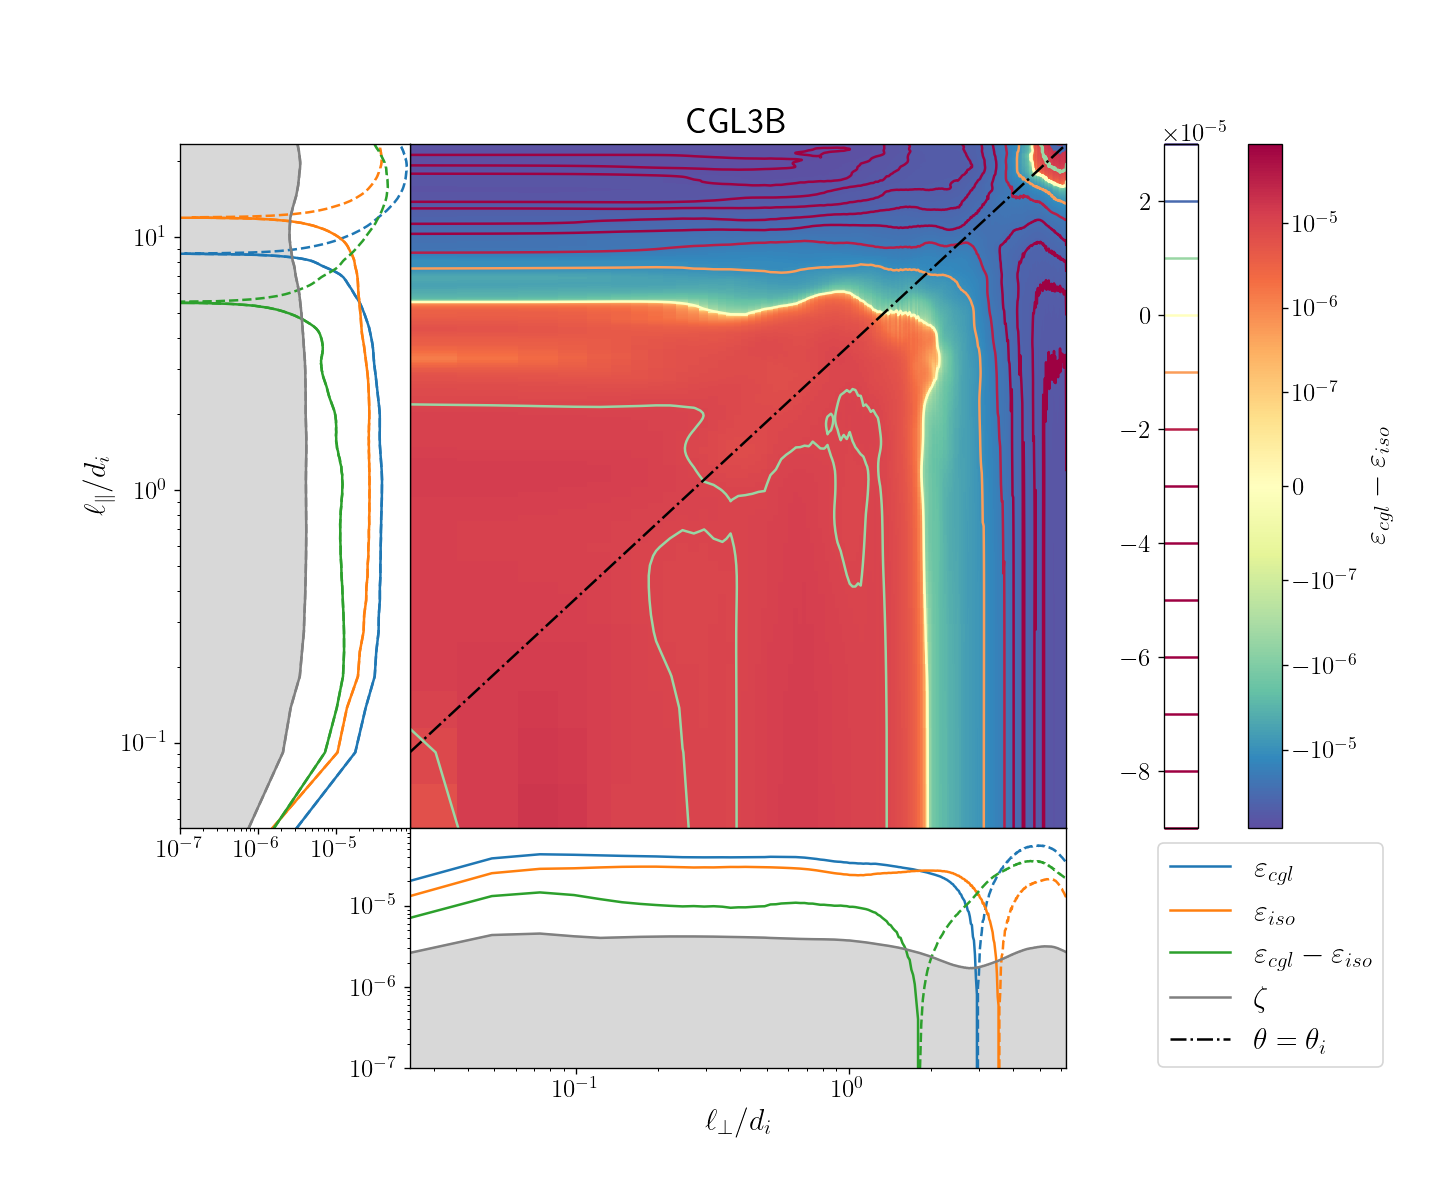
\includegraphics[width=0.95\linewidth,trim=0cm 2cm 0cm 3.5cm, clip=true]{./Part_3/images_ch3/CGL3B_panel_isocgl}
 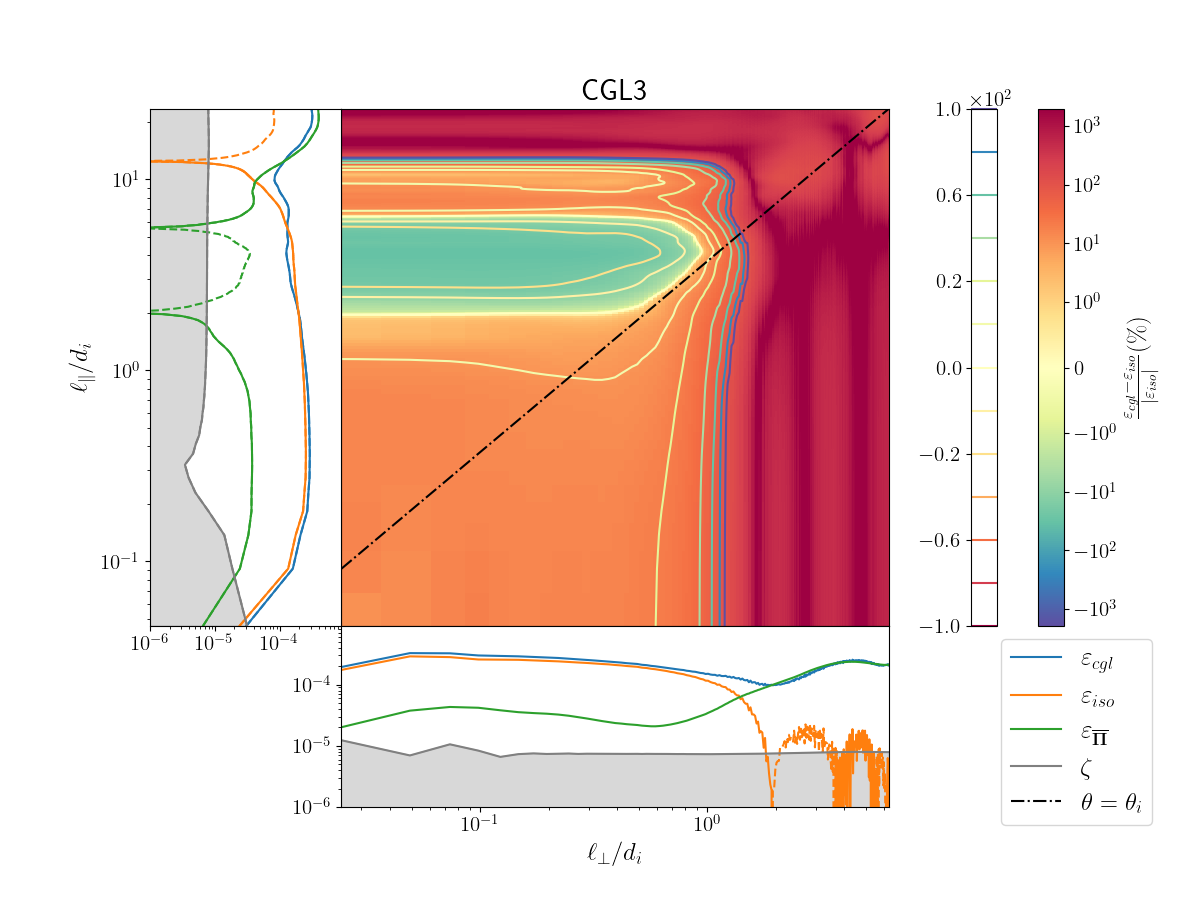
\includegraphics[width=0.95\linewidth,trim=1cm 1cm 0cm 2cm, clip=true]{./Mainmatter/Part_3/images_ch3/CGL3_panel_isocgl_percent}
 \cprotect\caption{Simu : CGL3. Représentation \cacro{2D} en fonction de \ensuremath{\ell_{\perp}} et \ensuremath{\ell_{\parallel}} de \ensuremath{\varepsilon_{cgl}-\varepsilon_{iso}} par rapport à \ensuremath{|\varepsilon_{iso}|} en \ensuremath{\%}, entourée des représentations \cacro{1D} en fonction de \ensuremath{\ell_{\perp}} (bas) et \ensuremath{\ell_{\parallel}} (gauche) de \ensuremath{\varepsilon_{iso}} (orange), \ensuremath{\varepsilon_{cgl}} (bleu),  \ensuremath{\varepsilon_{\overline{\boldsymbol{\Pi}}}} (vert) et \ensuremath{\zeta} (gris).}
 \label{fig:trip_CGL3}
 \end{figure}
 
 À partir de ces figures, on peut définir une zone inertielle où $\varepsilon_{cgl}$ sera quasi-constant pour chaque simulation. Pour CGL1, elle s'étend entre $\ell_{\perp} \in [\num{1};\num{20}]$ et $\ell_{\parallel} \in [\num{10};\num{60}]$, pour CGL2 entre $\ell_{\perp} \in [\num{1};\num{6}]$ et $\ell_{\parallel} \in [\num{2};\num{40}]$, et pour CGL3 entre $\ell_{\perp} \in [\num{0.1};\num{1}]$ et $\ell_{\parallel} \in [\num{0.2};\num{2}]$. Les variations que l'on pourra observer en dehors de ces domaines seront sous influence dissipative ou dans la zone de forçage. On remarque que la zone inertielle de CGL1 et CGL2 couvrent les échelles \cacro{MHD} et celle de CGL3, les échelles \cacro{Hall}. Dans ces zones, la contribution de $\varepsilon_{\overline{\boldsymbol{\Pi}}}$ au taux de cascade totale est en valeurs absolues d'environ $\SI{10}{\%}$ de $\varepsilon_{iso}$ pour CGL1 et CGL3, et entre $\SI{2}{\%}$ et $\SI{20}{\%}$ pour CGL2 (on prendra la valeur médiane : $\SI{10}{\%}$). Ce niveau reste donc constant. 
 
 Cependant, une différence de taille apparaît autour des grandes échelles de CGL3 (\figref{fig:trip_CGL3}) : $\varepsilon_{\overline{\boldsymbol{\Pi}}}$ augmente autour de $\num{10}$ fois la valeur de $\varepsilon_{iso}$. En pratique, on ne regarde pas ce qu'il se passe à ces échelles car elles sont impactées par l'injection d'énergie dans la cascade qui a tendance à faire fortement fluctuer les résultats provenant des lois calculées jusqu'à présents dans la littérature. Donc a priori, cette augmentation n'aurait pas un sens physique généralisable et serait plus spécifique à l'outil numérique. Pourtant, contrairement à l'impact du forçage observé dans la section \ref{sec-322}, il n'est pas oscillant et il provient spécifiquement de la contribution anisotrope. On s'est alors posé la question de son origine et de sa nature.
 
 Une autre différence est visible. Sur la représentation \sacro{2D} de CGL3 (\figref{fig:trip_CGL3}), la contribution anisotrope est positive quasiment partout à l'exception d'une \og bulle \fg{} accrochée à la direction parallèle. Tandis que pour CLG1 et CGL2 (\figref{fig:trip_CGL1-2}), un changement de signe de $\varepsilon_{\overline{\boldsymbol{\Pi}}}$ dans la zone inertielle \cacro{MHD} ($\ell > d_i$) semble indiquer une échelle caractéristique. Aux plus petites échelles, il est positif et puis devient négatif. L'emplacement de ce changement de signe est situé autour de $\ell^{s}_{\perp} \sim 2d_i$ dans la direction perpendiculaire. Dans la direction parallèle, le changement de signe a lieu en $\ell^{s}_{\parallel} \sim 20d_i$ pour CGL1, $\ell^{s}_{\parallel} \sim 80d_i$ pour CGL2. Trois éléments pourraient potentiellement expliquer ces observations. 
Tout d'abord, en présence d'un champ magnétique, le développement de la cascade est anisotrope comme on peut facilement le visualiser sur les cartes de \cite{manzini_local_2022}. Cela pourrait venir expliquer l'observation $\ell^{s}_{\perp}<\ell^{s}_{\parallel}$. Ensuite, l'angle d'injection $\theta_i$ étant inférieur à $\ang{45}$, l'énergie n'est pas injectée isotropiquement dans la simulation. Il diffère d'ailleurs entre CGL1 ($\ang{7}$) et CGL2-CGL3 ($\ang{15}$). Si le premier élément est validé, cela pourrait impliquer que l'angle d'injection pourrait venir contrer ou amplifier l'anisotropie de $\varepsilon_{\overline{\boldsymbol{\Pi}}}$. Enfin, entre CGL2 et CGL3, la gamme d'échelles diffère ainsi que le niveau énergétique ($E_{sup}$), plus important pour CGL3.

 Le comportement dans la direction parallèle semblant plus complexe que celui de la direction perpendiculaire, on s'est focalisé sur la compréhension de cette dernière.
 Puisque le changement de signe a lieu près de la zone \cacro{Hall}, on s'est demandé si le comportement de CGL2 et celui de CGL3 ne se complétaient pas : l'augmentation présente dans CGL3 serait-elle le début d'une bosse qui ensuite se répercuterait aux échelles  \cacro{MHD} où sa diminution irait jusqu'à engendrer un croisement de $\varepsilon_{cgl}$ et $\varepsilon_{iso}$ et un changement de signe de $\varepsilon_{\overline{\boldsymbol{\Pi}}}$ ? Ce point est intéressant, car une telle bosse pourrait être la signature d'instabilités qui viendraient injecter de l'énergie aux échelles ioniques. Cette première question est mise en doute par le comportement de CGL1 et CGL2 : une augmentation similaire semble apparaître dans $\varepsilon_{\overline{\boldsymbol{\Pi}}}$  mais avec un signe opposé et une intensité moindre n'influant que très peu sur $\varepsilon_{cgl}$. Si c'est bien le même effet que pour CGL3, il serait alors accroché aux échelles de forçage. 
 Plus de questions que de réponses émergent donc de ces simulations, elles ont emmené l'analyse dans diverses directions nécessitant de nouvelles simulations : 
 \begin{itemize}
     \item le niveau de la zone inertielle changera-t-il si l'on initialise la simulation avec une pression anisotropique ($a_{piI} \neq 1$) ? 
     \item l'augmentation à grande échelle est-elle accrochée aux échelles de forçage ?
    \item le changement de signe de  $\varepsilon_{\overline{\boldsymbol{\Pi}}}$ est-il lié à la proximité de la frontière entre les zones \cacro{MHD} et \cacro{Hall} ?
     \item ces différences sont-elles des signatures de phénomène physique ? Sont-elles liées ?
 \end{itemize}
 Avant de se lancer dans de nouvelles simulations, d'autres élements peuvent être étudiés. Ils font l'objet des sections suivantes.  
 
 \subsection{Détail de la contribution de l'anisotropie de pression}
 
 \begin{figure}[!ht]
  \centering
  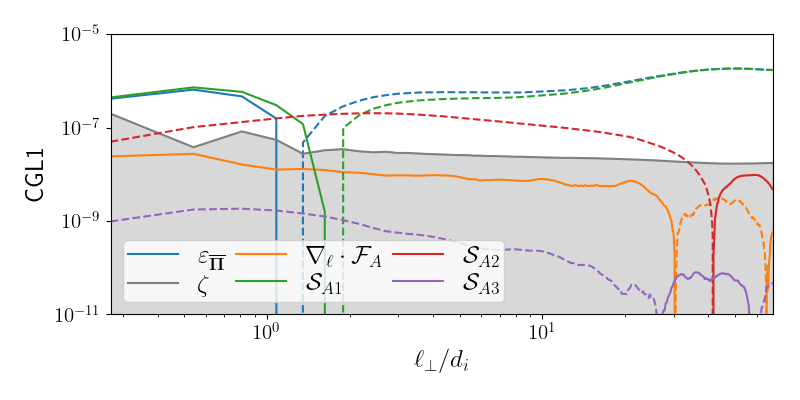
\includegraphics[width=0.9\linewidth,trim=0cm 0cm 0cm 0.5cm, clip=true]{./Mainmatter/Part_3/images_ch3/CGL1_compa_cgl}
 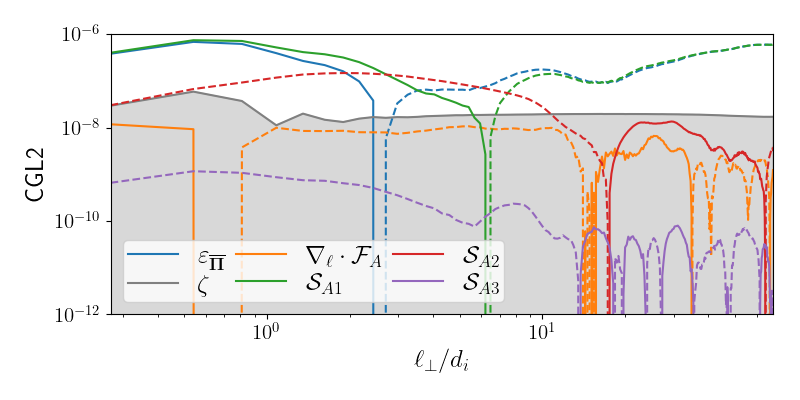
\includegraphics[width=0.9\linewidth,trim=0cm 0cm 0cm 0.5cm, clip=true]{./Mainmatter/Part_3/images_ch3/CGL2_compa_cgl}
  \includegraphics[width=0.9\linewidth,trim=0cm 0cm 0cm 0.5cm, clip=true]{./Mainmatter/Part_3/images_ch3/CGL3_compa_cgl}
 \cprotect\caption{Simu : CGL1 (haut), CGL2 (milieu) et  CGL3 (bas). Représentation \cacro{1D} en fonction de \ensuremath{\ell_{\perp}} du détail de \ensuremath{\varepsilon_{\overline{\boldsymbol{\Pi}}}} (bleu). Orange : \ensuremath{\nabla_{\boldsymbol{\ell}} \cdot \boldsymbol{\mathcal{F}_A}}. Vert : \ensuremath{\mathcal{S}_{A1}}. Rouge : \ensuremath{\mathcal{S}_{A2}}. Violet : \ensuremath{\mathcal{S}_{A3}}. Gris : niveau d'erreur \ensuremath{\zeta}. Les termes présents dans la zone grise délimitée par \ensuremath{\zeta} sont supposés négligeables. }
 \label{fig:detail_simu_CGL1-2}
 \end{figure}
 
 Sur la \figref{fig:detail_simu_CGL1-2}, est indiqué le détail de $\varepsilon_{\overline{\boldsymbol{\Pi}}}$ (bleu). On remarque que sont comportement est dominé par $\mathcal{S}_{A1}$ tandis que $\nabla_{\boldsymbol{\ell}} \cdot \boldsymbol{\mathcal{F}_A}$ et $\mathcal{S}_{A2}$ fluctuent autour de $\zeta$. Ils peuvent légèrement influencer $\varepsilon_{\overline{\boldsymbol{\Pi}}}$ lorsque $\mathcal{S}_{A1}$ s'affaiblit pour changer de signe, comme on peut le voir sur les résultats de CGL1 et CGL2. $\mathcal{S}_{A3}$ est, quant-à-lui, généralement négligeable. La contribution de l'anisotropie de pression et son comportement est donc principalement portée par le terme source qui survit dans la limite incompressible. Cela concorde avec la quasi-incompressibilité des simulations : l'écart-type de la densité est entre $\SI{2}{\%}$ (CGL1 et CGL2) et $\SI{8}{\%}$ (CGL3) de la moyenne. $\mathcal{S}_{A1}$ et $\varepsilon_{\overline{\boldsymbol{\Pi}}}$ doivent donc se comporter en accord avec la limite quasi-incompressible \eqref{eq:turb_cpinc_gyr1} obtenue dans le Chapitre \ref{ch-22} : 
 \begin{equation}
     \varepsilon_{\overline{\boldsymbol{\Pi}}} \simeq \mathcal{S}_{A1} \simeq \frac{\beta_0}{4}  \left< \delta \left(\left(p_{\parallel i } - p_{\perp i }\right)\left( \boldsymbol{b} \boldsymbol{b} - \frac{1}{3}  \overline{\boldsymbol{I}} \right) \right):\delta \left(\nabla \boldsymbol{v} \right)\right>
 \end{equation}
 Comprendre le comportement de ce terme est complexe puisqu'il dépend des fluctuations de la direction du champ magnétique $\boldsymbol{b}$ pondérées par l'anisotropie de la pression et distribuées sur les variations du gradient de la vitesse. $p_{\parallel i } - p_{\perp i }$ portant l'influence de l'anisotropie de pression de ce terme sur la loi exacte et pouvant s'écrire $1-a_{pi}$, on s'est intéressé au comportement statistique de $a_{pi}$. On remarque que seule la direction du champ magnétique influe sur ce terme et non son amplitude.
 
 Ces résultats sont retrouvés dans les simulations qui seront étudiées par la suite (voir Annexe \ref{an:Pi}).
 
 \subsection{Comportement statistique des pressions}
 
 La \tabref{tab:stat_CGL} résume la statistique (moyenne $\pm$ écart-type) des valeurs de la densité, de l'anisotropie de pression ionique $a_{pi} = \frac{p_{\perp i}}{p_{\parallel i}}$, et du paramètre $\beta_{\parallel} = \frac{p_{\parallel i}}{p_{m}}$ pour chaque simulation. Sur la figure \figref{fig:diag_simu_CGL}, est tracée la dispersion en fonction de $a_{pi}$ et $\beta_{\parallel}$, des simulations. Ces histogrammes \sacro{2D} prennent la forme de trois courbes de niveau formant des ovales concentriques. Le plus large contient tous les couples $\{\beta_{\parallel};a_{pi}\}$ existant dans la simulation, l'intermédiaire et le plus petit sont associés à des pourcentages du maximum de l'histogramme : $\SI{50}{\%}$ et $\SI{99}{\%}$. Sur cette figure, les critères des instabilités miroir et firehose ainsi que l'horizontale $a_{pi} =  1$ sont aussi affichés. Le critère firehose est le critère calculé dans le chapitre \ref{ch-21}, sa position sera affectée par l'effet \cacro{Hall}. Le critère miroir prend en compte la présence de la pression électronique isotherme $p_e = \rho$ et est paramétrisé par l'équation \eqref{eq:crit_miroir_elec}. Les simulations que l'on étudie ici sont données en 
 gris (CGL1), bleu (CGL2) et orange (CGL3) et correspondent aux première, deuxième et quatrième lignes du tableau. 
  \begin{table}[!ht]
 \begin{center}
 \begin{tabular}{ c|c|c|c } 
 Name & $\rho$ & $a_{pi}$  & $\beta_{\parallel}$\\
 \hline
 CGL1 & $\num{1}\pm \num{0.02}$ & $\num{1.1}\pm \num{0.1}$ & $\num{0.9}\pm \num{0.1}$ \\
 CGL2 & $\num{1}\pm \num{0.02}$ & $\num{1.1}\pm \num{0.1}$ & $\num{0.9}\pm \num{0.1}$   \\
 CGL3B & $\num{1}\pm \num{0.04}$ & $\num{1.3}\pm \num{0.3}$ & $\num{0.8}\pm \num{0.2}$   \\
 CGL3 & $\num{1}\pm \num{0.08}$ & $\num{2.2}\pm \num{0.5}$ & $\num{0.6}\pm \num{0.3}$  \\
 CGL5 & $\num{1}\pm \num{0.02}$ & $\num{2.1}\pm \num{0.1}$ & $\num{0.6}\pm \num{0.1}$  \\
 CGL6 & $\num{1}\pm \num{0.02}$ & $\num{3.97}\pm \num{0.5}$ & $\num{1.01}\pm \num{0.2}$  \\
 \end{tabular}
 \caption{Moyenne et écart-type de la densité, du taux d'anisotropie ionique $a_{pi} = \frac{p_{\perp i}}{p_{\parallel i}}$ et du paramètre $\beta_{\parallel} = \frac{p_{\parallel i}}{p_{m}}$ pour chaque simulation, à la date $t$. }\label{tab:stat_CGL}
 \end{center}
 \end{table}
 \begin{figure}[!ht]
  \centering
 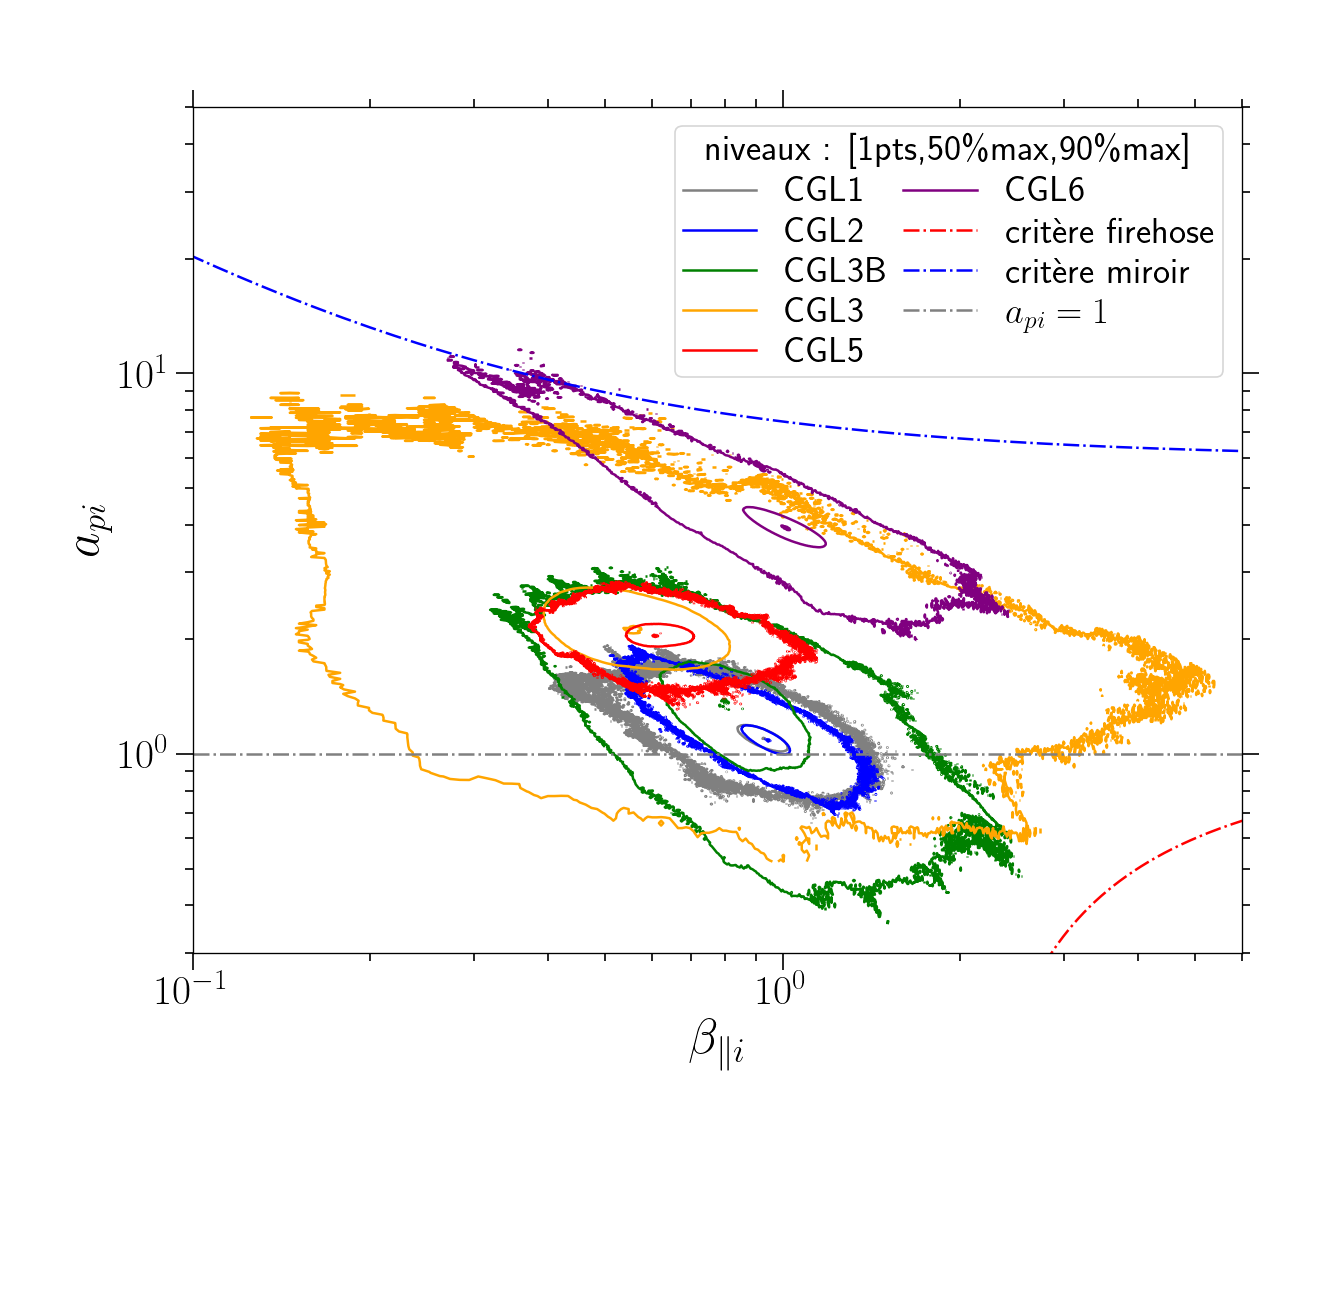
\includegraphics[width=0.8\linewidth,trim=1cm 7cm 2cm 1cm, clip=true]{./Mainmatter/Part_3/images_ch3/diag_apbeta}
 \cprotect\caption{Diagramme \ensuremath{a_{pi}-\beta_{\parallel}} contenant l'histogramme \sacro{2D} des simulations sous la forme de courbes de niveau centrées sur le couple moyen. Le critère miroir est paramétrisé par l'équation \eqref{eq:crit_miroir_elec} qui prend en compte les électrons isothermes. Le critère firehose est le critère \cacro{CGL} calculé dans le Chapitre \ref{ch-21}. }
 \label{fig:diag_simu_CGL}
 \end{figure} 
 
 On remarque que les trois simulations se sont écartées de leurs valeurs d'initialisation, $a_{piI} = 1$ et $\beta_{\parallel I} = 1$. $ \mathcal{S}_{A1}$ ne dépendant pas de $p_m$, on ne s'est pas attardé sur $\beta_{\parallel} = 1$.  Les distributions de CGL1 et de CGL2 sont quasiment identiques et très proches des valeurs initiales. CGL3 s'est quant-à-elle bien décalée et montre une moyenne $a_{pi0}\sim 2$, sa distribution est aussi beaucoup plus large avec quelques points proches du critère miroir. L'augmentation de la pression a lieu dès les premiers temps de la simulation puis reste stable. La raison d'un tel comportement est encore sujette à question : notre conjecture est qu'il est dû à l'énergie présente dans CGL3. Cette dernière est en effet forcée avec des ondes plus intenses et telle que l'énergie dans le système soit trois fois supérieure à celle dans CGL1 ou CGL2 (voir resp. $A_f$ et $E_{sup}$). Entre les points proches du critère miroir et l'augmentation de la moyenne et de l'écart-type de $a_{pi}$, beaucoup d'éléments pourraient être à l'origine de la différence de comportement de la contribution anisotrope. Ces résultats motivent d'autant plus l'obtention de nouvelles simulations. 
 
 \section{De nouvelles simulations}\label{sec-333}
 
 Trois nouvelles simulations ont été utilisées : CGL3B, CGL5 et CGL6. CGL5 et CGL6 ont été conçues et lancées pour répondre à certaines de nos questions. Comme indiqué dans le Chapitre \ref{ch-31}, obtenir des résultats de simulation valables pour une étude de turbulence prend du temps, c'est-à-dire plusieurs mois en comptant l'ajustement des paramètres d'hyperdissipation et, sachant qu'à chaque augmentation de la résolution, le temps de calcul était au moins multiplié par huit. Ainsi, d'une semaine de calcul pour faire converger le spectre associé à une résolution $258^2\times 512$, on passe à un ou deux mois pour $512^2 \times 1024$. Par conséquent, les résultats présentés ici sont récents et leur interprétation est encore en cours. 
 
 \subsection{Moins d'énergie que CGL3 : CGL3B}
 \begin{figure}[!ht]
  \centering
  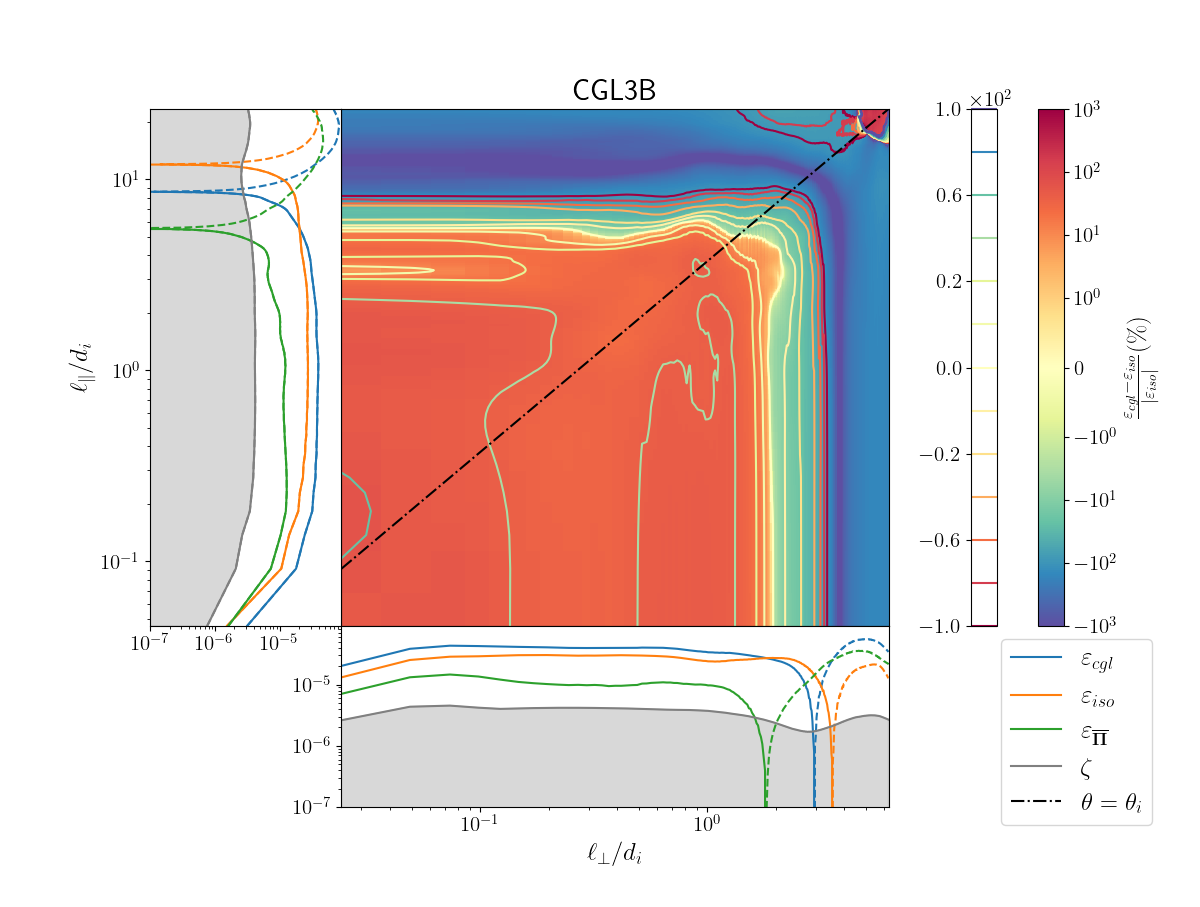
\includegraphics[width=0.95\linewidth,trim=1cm 1cm 0cm 2cm, clip=true]{./Mainmatter/Part_3/images_ch3/CGL3B_panel_isocgl_percent}
 %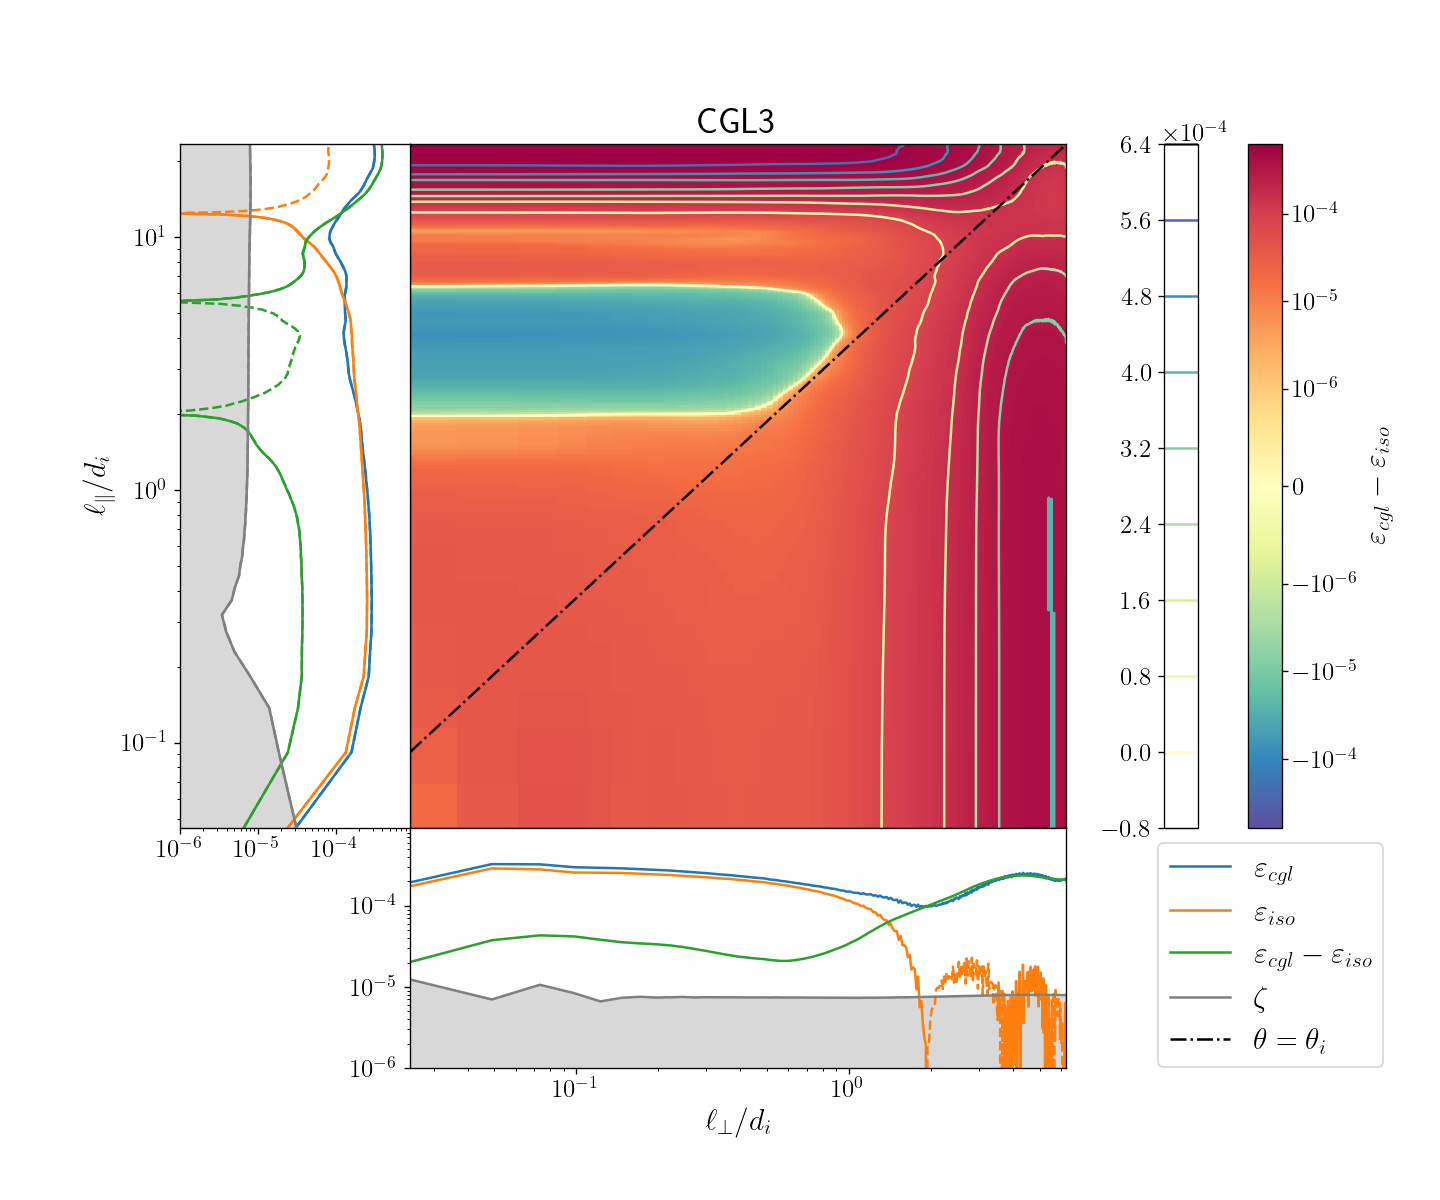
\includegraphics[width=0.95\linewidth,trim=0cm 2cm 0cm 3.5cm, clip=true]{./Part_3/images_ch3/CGL3_panel_isocgl}
 \cprotect\caption{Simu : CGL3B. Représentation \sacro{2D} en fonction de \ensuremath{\ell_{\perp}} et \ensuremath{\ell_{\parallel}} de \ensuremath{\varepsilon_{cgl}-\varepsilon_{iso}} par rapport à \ensuremath{|\varepsilon_{iso}|} en \ensuremath{\%}, entourée des représentations \cacro{1D} en fonction de \ensuremath{\ell_{\perp}} (bas) et \ensuremath{\ell_{\parallel}} (gauche) de \ensuremath{\varepsilon_{iso}} (orange), \ensuremath{\varepsilon_{cgl}} (bleu), \ensuremath{\varepsilon_{\overline{\boldsymbol{\Pi}}}} (vert) et \ensuremath{\zeta} (gris). }
 \label{fig:trip_CGL3B}
 \end{figure}
 Tout d'abord, CGL3B est une version moins énergétique de CGL3. La gamme d'échelle est donc la même, seul le forçage et par conséquent la dissipation sont affaiblis. Cette simulation est, elle aussi, initialisée telle que $a_{piI} = 1$. Sur le diagramme de la \figref{fig:diag_simu_CGL}, elle est indiquée en vert : sa moyenne, $a_{pi0} \sim 1.5$,  est entre celle de CGL2 et CGL3, et sa distribution inclue celle de CGL2 mais est moins étalée que celle de CGL3. On s'attend donc à voir les différences les plus importantes entre les résultats de l'étude des lois exactes de CGL2 et de CGL3 s'atténuer si $a_{pi}$ a de l'importance dans l'expression de la correction anisotrope.  Le triptyque fait l'objet de la \figref{fig:trip_CGL3B}. %Les contributions purement compressibles de $\varepsilon_{\overline{\boldsymbol{\Pi}}}$ étant ici aussi négligeable, on ne donnera pas son détail.
 
 À première vue, en regardant la représentation \sacro{2D}, on sait que l'on a un comportement similaire à CGL2. Le croisement entre $\varepsilon_{cgl}$ et $\varepsilon_{iso}$ dû au changement de signe de $\varepsilon_{\overline{\boldsymbol{\Pi}}}$ est toujours présent dans la zone \cacro{MHD}. Comme pour CGL3, cette zone est aussi la zone de forçage. Dans cette zone, on remarque une augmentation de la contribution venant dominer $\varepsilon_{iso}$. Si ces deux éléments ne sont pas des artefacts dus à l'oscillation du forçage, cela signifie que, contrairement à CGL3 et similairement à CGL1 et CGL2, le changement de signe a lieu avant l'augmentation, et cela tend à indiquer que l'augmentation présente dans CGL3 est intrinsèque à la zone de forçage.
 
 La zone inertielle est située entre $\ell_{\perp} \in [\num{0.1};\num{2}]$ et $\ell_{\parallel} \in [\num{0.2};\num{4}]$. Cette fois-ci, $\varepsilon_{\overline{\boldsymbol{\Pi}}}$ contribue à $\SI{30}{\%}$ de $\varepsilon_{iso}$. On a donc un facteur 3 par rapport aux $\SI{10}{\%}$ relevés pour les autres simulations. Ce résultat, significatif, indique que l'anisotropie de pression semble affecter la zone inertielle mais interpelle aussi car, pour une simulation que tout semble placer entre CGL2 et CGL3, l'effet de l'anisotropie de pression sur la zone inertielle en est éloigné. La source d'un tel comportement est encore en cours de discussion. 
  
 % \begin{figure}[!ht]
 %  \centering
 % 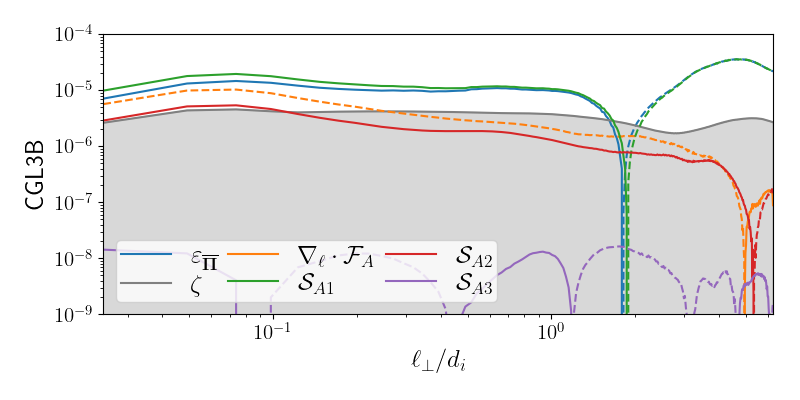
\includegraphics[width=1\linewidth,trim=0cm 1cm 0cm 1cm, clip=true]{./Part_3/images_ch3/CGL3B_compa_cgl}
 % % \includegraphics[width=1\linewidth,trim=0cm 1cm 0cm 1cm, clip=true]{./Part_3/images_ch3/CGL3_compa_cgl}
% \cprotect\caption{Représentation \acs{1D} en fonction de $\ell_{\perp}$ du détail de $\varepsilon_{\overline{\boldsymbol{\Pi}}}$ (bleu). Orange : $\nabla_{\boldsymbol{\ell}} \cdot \boldsymbol{\mathcal{F}_A}$. Vert : $\mathcal{S}_{A1}$. Rouge : $\mathcal{S}_{A2}$. Violet : $\mathcal{S}_{A3}$. Gris : niveau d'erreur $\zeta$. Les termes présents dans la zone grise délimitée par $\zeta$ sont supposés négligeables. Simu : CGL3B. }
% \label{fig:detail_simu_CGL3B}
% \end{figure}

\subsection{Une gamme d'échelle intermédiaire : CGL5}
\begin{figure}[!ht]
 \centering
 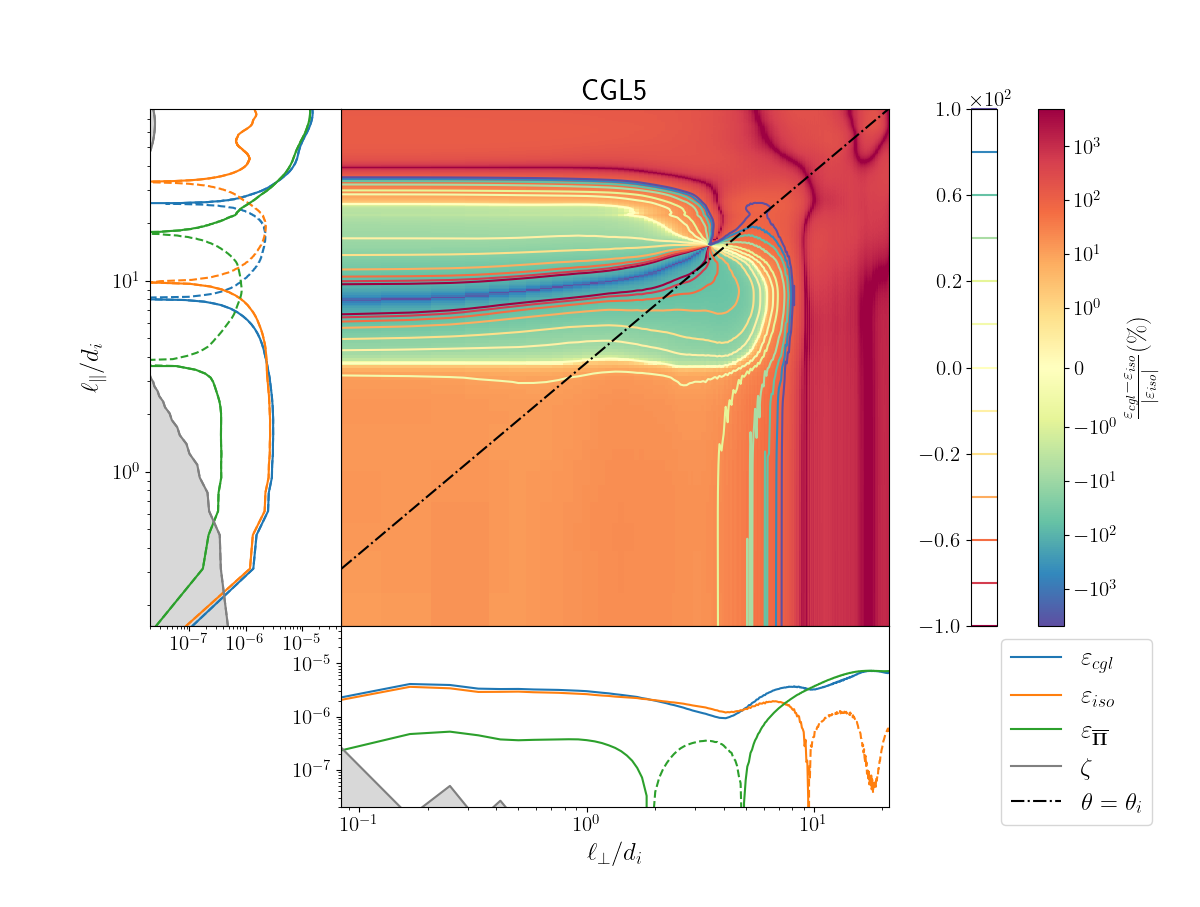
\includegraphics[width=0.95\linewidth,trim=1cm 1cm 0cm 2cm, clip=true]{./Mainmatter/Part_3/images_ch3/CGL5_panel_isocgl_percent}
 \cprotect\caption{Simu : CGL5. Représentation \sacro{2D} en fonction de \ensuremath{\ell_{\perp}} et \ensuremath{\ell_{\parallel}} de \ensuremath{\varepsilon_{cgl}-\varepsilon_{iso}} par rapport à \ensuremath{|\varepsilon_{iso}|} en \ensuremath{\%}, entourée des représentations \cacro{1D} en fonction de \ensuremath{\ell_{\perp}} (bas) et \ensuremath{\ell_{\parallel}} (gauche) de \ensuremath{\varepsilon_{iso}} (orange), \ensuremath{\varepsilon_{cgl}} (bleu), \ensuremath{\varepsilon_{\overline{\boldsymbol{\Pi}}}} (vert) et \ensuremath{\zeta} (gris). }
\label{fig:trip_CGL5}
\end{figure}

 La gamme d'échelles accessible via CGL5 est située entre celles de CGL2 et celles de CGL3 afin de couvrir la transition entre la zone \cacro{MHD} et la zone \cacro{Hall}, tout en gardant éloignées les échelles impactées par l'injection d'énergie. %Sur la \tabref{tab:stat_CGL}, on voit que sa compression est similaire à celle de CGL2, les termes purement compressibles seront encore une fois négligeables.
 L'écart-type de sa distribution est aussi de l'ordre de celui de CGL2, tout comme son étalement dans le diagramme de la \figref{fig:diag_simu_CGL}, mais sa position centrale y est plus proche de celle de CGL3. Le comportement observé pourrait donc être en faveur de la conjecture d'un impact de la moyenne de $a_{pi}$ ou de celle d'un impact des fluctuations sur la contribution du taux de cascade dépendant de l'anisotropie de pression. 
 
 % \begin{figure}[!ht]
 %  \centering
 %  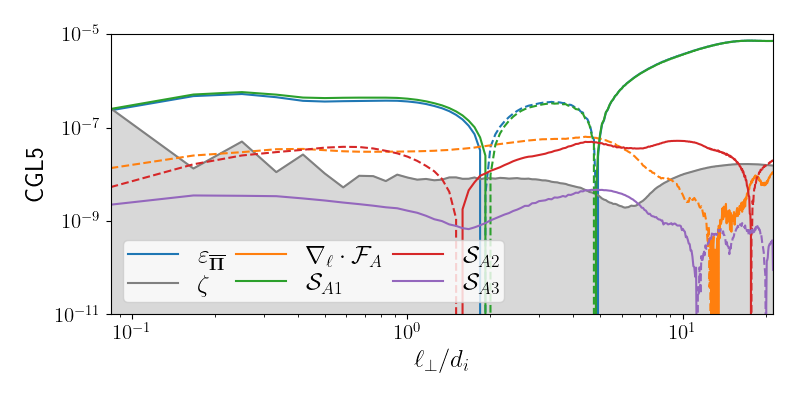
\includegraphics[width=1\linewidth,trim=0cm 1cm 0cm 1cm, clip=true]{./Part_3/images_ch3/CGL5_compa_cgl}
 % \cprotect\caption{Simu : CGL5. Représentation 1D en fonction de $\ell_{\perp}$ du détail de $\varepsilon_{\overline{\boldsymbol{\Pi}}}$ (bleu). Orange : $\nabla_{\boldsymbol{\ell}} \cdot \boldsymbol{\mathcal{F}_A}$. Vert : $\mathcal{S}_{A1}$. Rouge : $\mathcal{S}_{A2}$. Violet : $\mathcal{S}_{A3}$. Gris : niveau d'erreur $\zeta$. Les termes présents dans la zone grise délimitée par $\zeta$ sont supposés négligeables. }
 % \label{fig:detail_simu_CGL5}
 % \end{figure}
 
 Sur le triptyque obtenu pour CGL5 (\figref{fig:trip_CGL5}), on observe un comportement similaire à celui de CGL3. Dans la zone inertielle ($\ell_{\perp} \in [\num{0.3};\num{5}]$\footnote{La taille de la zone inertielle perpendiculaire dans la représentation \cacro{1D} de la \figref{fig:trip_CGL5} est réduite à cause de la \og bulle \fg{} négative parallèle et du filtrage angulaire. La valeur maximale est donc estimée à partir de la représentation \sacro{2D}.}), la contribution de $\varepsilon_{\overline{\boldsymbol{\Pi}}}$ est de l'ordre de $\SI{10}{\%}$ de $\varepsilon_{iso}$. Ces résultats confirment que le comportement de CGL3 n'est pas un cas particulier et se placent en faveur de la moyenne de $a_{pi}$ plutôt que de ses fluctuations. De plus, l'augmentation à grande échelle visible pour CGL3 s'est déportée avec le forçage, confirmant qu'elle est intrinsèque à la zone d'injection de l'énergie dans la cascade.  


\subsection{Une initialisation anisotrope $a_{piI} = 4$ : CGL6}
\begin{figure}[!ht]
 \centering
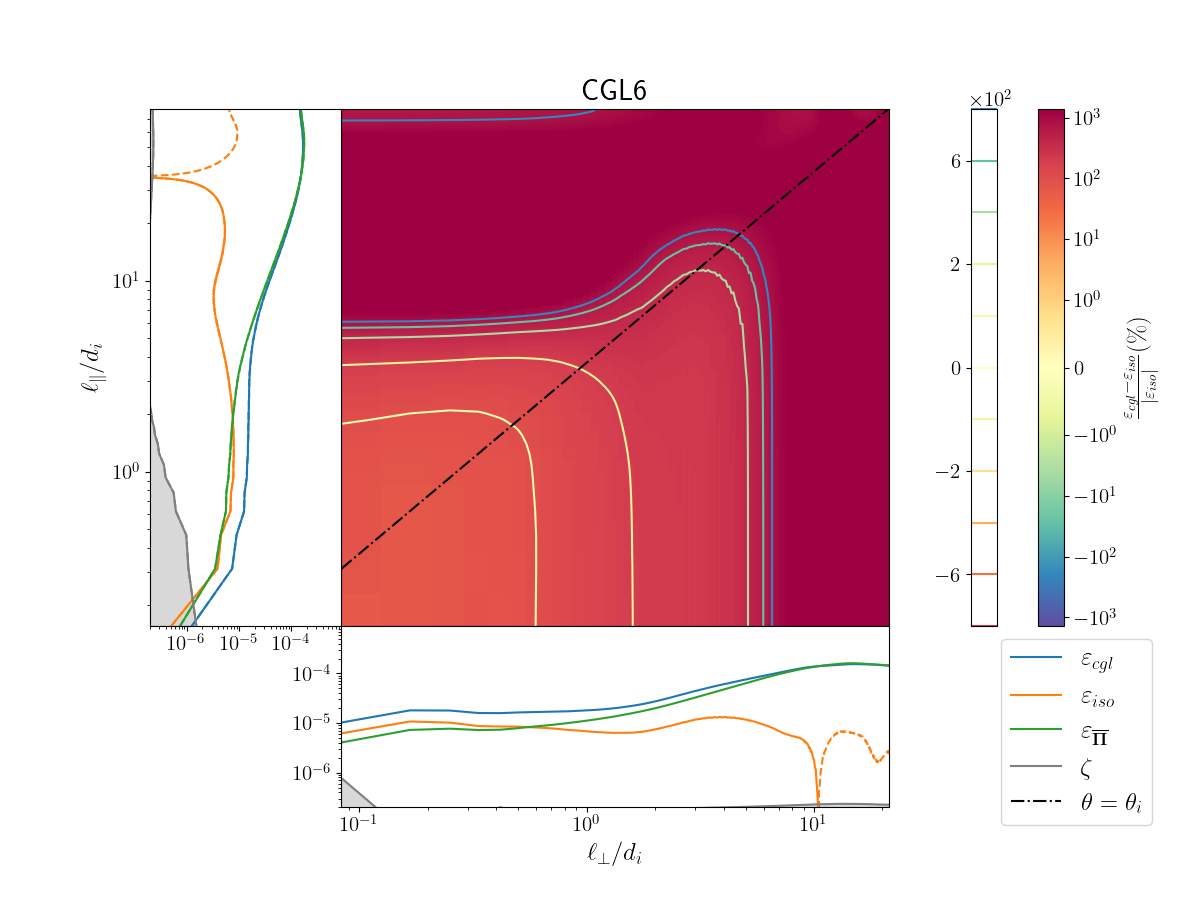
\includegraphics[width=0.95\linewidth,trim=1cm 1cm 0cm 2cm, clip=true]{./Mainmatter/Part_3/images_ch3/CGL6_panel_isocgl_percent}
\cprotect\caption{Simu : CGL6. Représentation \sacro{2D} en fonction de \ensuremath{\ell_{\perp}} et \ensuremath{\ell_{\parallel}} de \ensuremath{\varepsilon_{cgl}-\varepsilon_{iso}} par rapport à \ensuremath{|\varepsilon_{iso}|} en \ensuremath{\%}, entourée des représentations \cacro{1D} en fonction de \ensuremath{\ell_{\perp}} (bas) et \ensuremath{\ell_{\parallel}} (gauche) de \ensuremath{\varepsilon_{iso}} (orange), \ensuremath{\varepsilon_{cgl}} (bleu), \ensuremath{\varepsilon_{\overline{\boldsymbol{\Pi}}}} (vert) et \ensuremath{\zeta} (gris). }
\label{fig:trip_CGL6}
\end{figure}
La dernière simulation lancée est CGL6. Elle est basée sur CGL5 mais initialisée avec une pression anisotrope : $a_{piI} = 4 $. Le but de cette simulation est double :
\begin{itemize}
    \item vérifier si l'un des comportements observés précédemment pour notre correction se maintient lorsque la simulation est initialisée anisotropiquement,
    \item se rapprocher du critère miroir.
\end{itemize}
Des valeurs de $a_{piI}$ plus importantes ont été testées, mais seule la simulation avec $a_{piI} = 4 $ a pu être numériquement stabilisée. 

 Comme on peut le voir sur la \tabref{tab:stat_CGL} et sur la \figref{fig:diag_simu_CGL} (violet), cette simulation se maintient au niveau de $a_{piI}$. En fait, c'est la seule simulation montrant un $a_{pi0}$ aussi proche de sa condition initiale, l'écart n'étant que de $\SI{3}{\%}$. Pour ce qui est du but de se rapprocher du critère miroir, le diagramme nous indique que quelques points de CGL6 sont situés au-dessus du critère miroir. Le développement d'instabilité miroir semble donc permis dans cette simulation. 
 
 Sur la \figref{fig:trip_CGL6},  $\varepsilon_{\overline{\boldsymbol{\Pi}}}$ est entièrement positif. Son niveau est de l'ordre de $\SI{70}{\%}$ de $\varepsilon_{iso}$ aux échelles inertielles, c'est-à-dire pour $\ell_{\perp} \in [\num{0.3};\num{1}]$. Il a donc bien augmenté par comparaison avec les $\SI{10}{\%}$ et $\SI{30}{\%}$ précédents. Par comparaison avec CGL5, la gamme d'échelles inertielles est réduite par l'augmentation de $\varepsilon_{\overline{\boldsymbol{\Pi}}}$ qui est plus étalée. %Les termes purement compressibles sont toujours de l'ordre de l'erreur numérique.


% \begin{figure}[!ht]
%  \centering
% 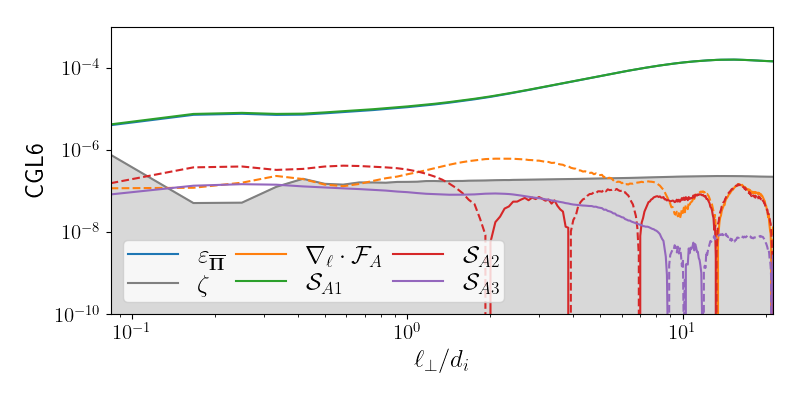
\includegraphics[width=1\linewidth,trim=0cm 1cm 0cm 1cm, clip=true]{./Part_3/images_ch3/CGL6_compa_cgl}
% \cprotect\caption{Simu : CGL6. Représentation 1D en fonction de $\ell_{\perp}$ du détail de $\varepsilon_{\overline{\boldsymbol{\Pi}}}$ (bleu). Orange : $\nabla_{\boldsymbol{\ell}} \cdot \boldsymbol{\mathcal{F}_A}$. Vert : $\mathcal{S}_{A1}$. Rouge : $\mathcal{S}_{A2}$. Violet : $\mathcal{S}_{A3}$. Gris : niveau d'erreur $\zeta$. Les termes présents dans la zone grise délimitée par $\zeta$ sont supposés négligeables. De haut en bas : CGL3, CGL5 et CGL6. }
% \label{fig:detail_simu_CGL6}
% \end{figure}

\section{Synthèse de l'étude préliminaire des simulations CGL-MHD-Hall-\ensuremath{\nabla P_e}}
\label{synth-33}

{\bf Les résultats présentés dans ce chapitre nous permettent de valider numériquement l'apport de la correction dépendant de l'anisotropie de pression dans le cas quasi-incompressible. Ils nous confirment aussi que, dans un cadre quasi-incompressible, le terme dominant est celui qui vient former la correction de \cacro{PP98} dans la limite incompressible gyrotrope (Chapitre \ref{ch-22}).} Cela implique que la première correction devant être appliquée dans un plasma quasi-incompressible tel que le vent solaire n'est peut-être pas la compression mais plutôt l'anisotropie de pression. Cette étude numérique n'est cependant qu'à un stade préliminaire. En effet, nous n'avons pas encore convergé sur l'interprétation d'un certain nombre d'éléments et, comme nous venons de le voir, elle soulève un nombre important de questions.


\begin{figure}[!ht]
 \centering
 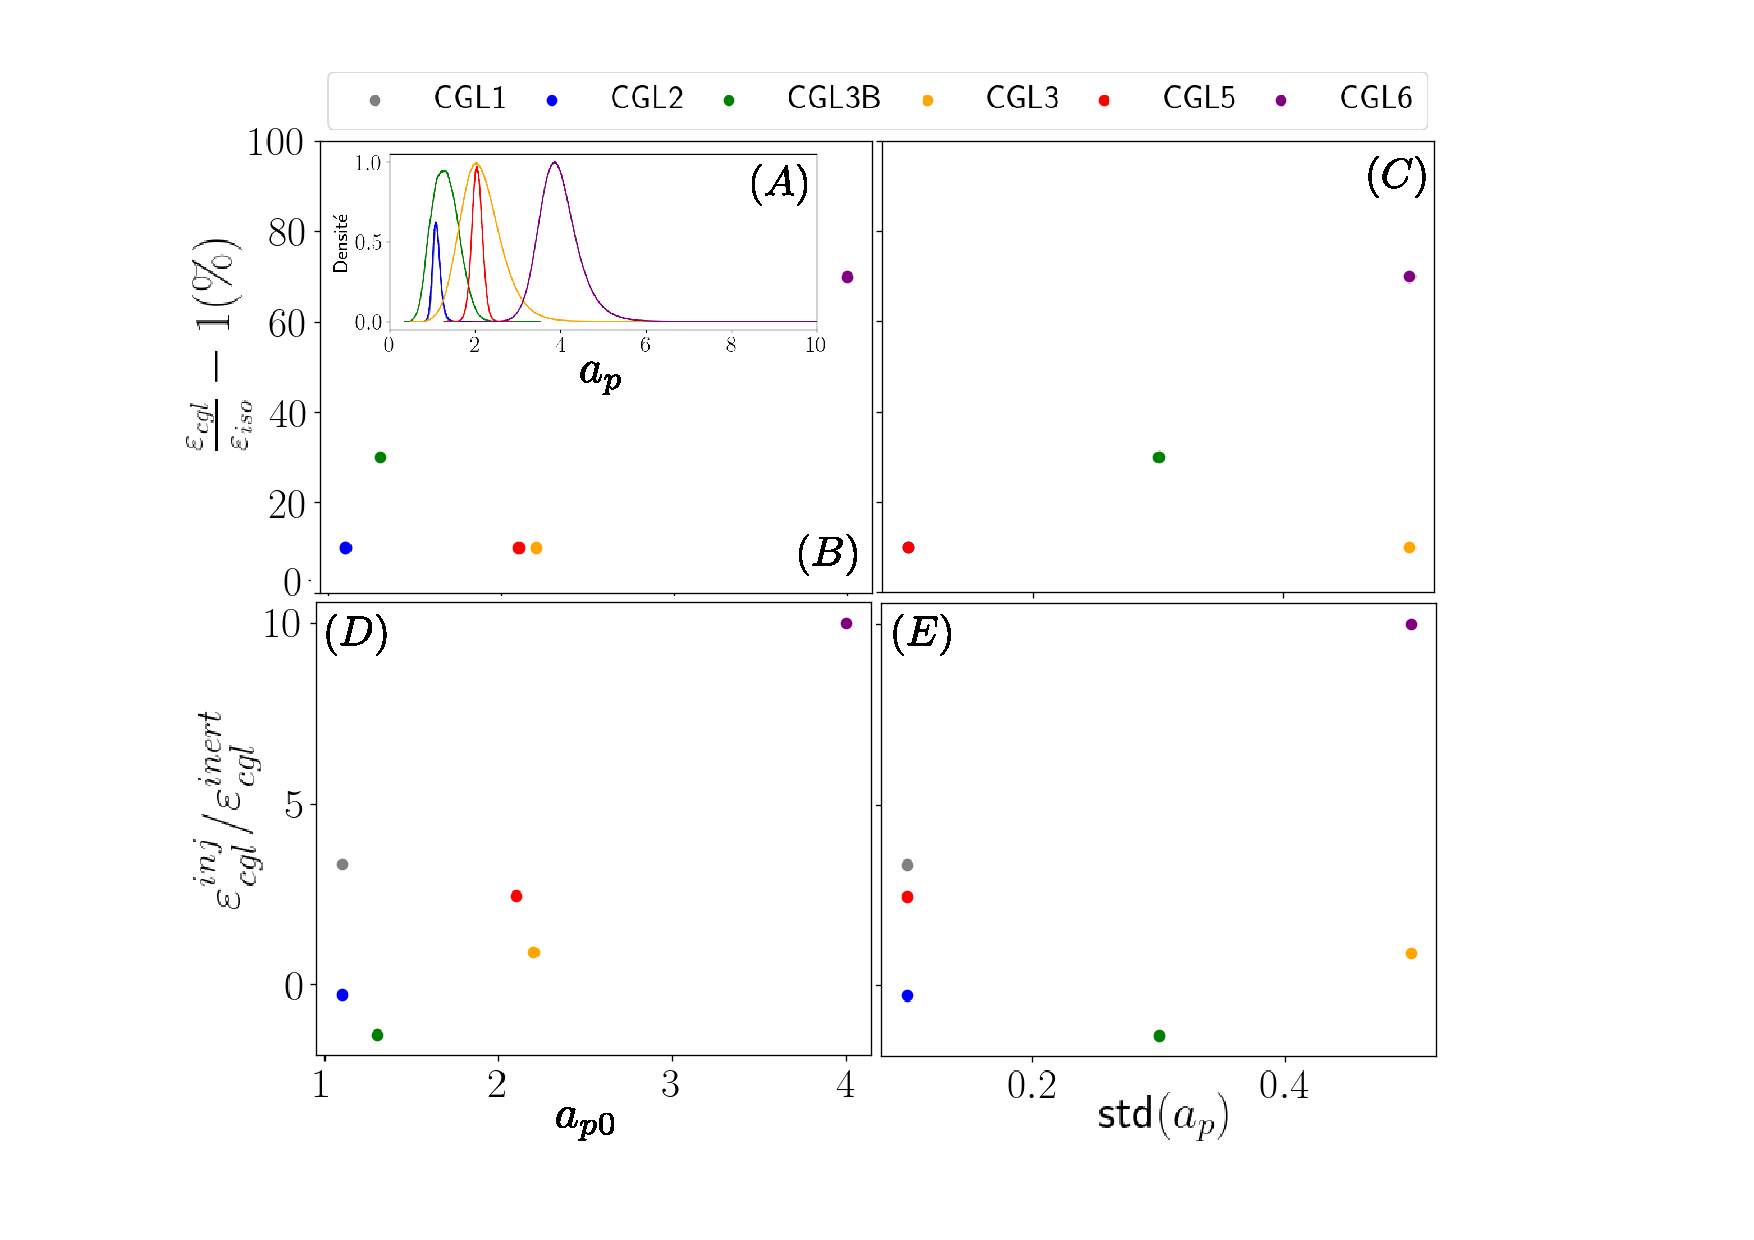
\includegraphics[width=0.9\linewidth,trim=3cm 1cm 5cm 1cm, clip=true]{./Mainmatter/Part_3/images_ch3/scattersimu}
\cprotect\caption{Résumé de l'étude préliminaire sur l'effet de l'anisotropie de pression sur le taux de transfert non linéaire en fonction de \ensuremath{a_{pi0}} (première colonne) et de \ensuremath{\text{std}(a_p)} (deuxième colonne). Chaque simulation est associée à une couleur (même association que pour la \figref{fig:diag_simu_CGL}). (A) : histogramme de \ensuremath{a_p}, CGL1 y est confondu avec CGL2. (B) et (C) : apport de la contribution de la pression anisotrope. (D) et (E) : impact de l'augmentation dans la zone de forçage de la contribution anisotrope sur le niveau du taux de transfert total mesuré dans la zone inertielle.}
\label{fig:scattersimu}
\end{figure}
 
 On propose une synthèse à travers la \figref{fig:scattersimu}. Sur le graphique $(A)$ sont repris les histogrammes de $a_{pi}$, (CGL1 y est confondu avec CGL2). Les simulations sont ordonnées par couleur et comportement : les simulations présentant un changement de signe sont en gris (CGL1), bleu (CGL2) et vert (CGL3B). Celles  montrant un signe quasiment isotrope à l'exception d'une \og bulle \fg{} dans la direction parallèle sont en jaune (CGL3) et rouge (CGL5). La dernière simulation, initialisée avec $a_{piI}  = 4$, montrant une contribution anisotrope entièrement positive, est donnée en violet (CGL6). Deux paramètres liés à la distribution de $a_{pi}$ ont été abordés : la moyenne $a_{pi0}$ (graphique $(B)$ et $(C)$) et l'écart-type $\text{std}(a_{pi})$ (graphique $(D)$ et $(E)$). En fonction de $a_{pi0}$, les simulations se comportant similairement restent groupées, contrairement à $\text{std}(a_{pi})$. $a_{pi0}$ semble donc être un meilleur paramètre que $\text{std}(a_{pi})$. Sur le graphique $(B)$, sont placées les estimations de la contribution anisotrope au taux de cascade dans la zone inertielle. On y observe que CGL3B et CGL6 s'écartent du résultat des autres simulations. Ce résultat est inattendu pour CGL3B (ou CGL3 et CGL5). Si $a_{pi0}$ est bien le paramètre important dans l'impact des anisotropies de pression sur la cascade et que CGL3B est bien valable et n'est pas une exception, alors il pourrait exister un processus qui viendrait inverser, pour quelques $a_{pi0}$, la tendance croissante de la contribution anisotrope dans la zone inertielle. Pour ce qui est du rapport entre le taux de transfert non linéaire estimé dans la zone de forçage et le taux de cascade inertielle (graphique (D)), il semble globalement croitre en fonction de $a_{pi0}$. Il serait intéressant d'y évaluer plus précisément l'impact de l'injection d'énergie afin de vérifier si un autre processus intervient. 
 
 Ces graphiques, contenant un nombre limité de points lié au nombre de simulations à disposition, ne sont, bien évidemment, que des outils de spéculation, synthétisant cette étude préliminaire et permettant de dégager des tendances pour lesquelles l'analyse pourra être approfondie.




% \section{Etude de spectre } \label{sec-334}

% Sachant que le forçage se fait avec des modes aléatoires de fréquences proches de celle du mode d'Alfvén et que des études telles celle de \cite{brodiano_spatiotemporal_2021} ont relié le choix de forçage aux ondes dominant la simulation, observer une cascade développée par des ondes d'Alfvén dans nos simulations serait tout à fait réaliste. Si l'on regarde les spectres de champs magnétiques parallèle et perpendiculaire de CGL2 par exemple (\figref{fig:spectre}), on remarque que le spectre d'énergie magnétique est dominé par les fluctuations perpendiculaires au champ magnétique ambiant et on y retrouve les pentes turbulentes en $-5/3$ (zone MHD) et en $-7/3$ (zone Hall).  Un tel résultat est une signature de la nature alfvénique de la cascade turbulente. Il n'est donc pas impossible que la correction d'anisotropie de pression soit dominé par la correction firehose. 
% \begin{figure}[!ht]
%  \centering
% 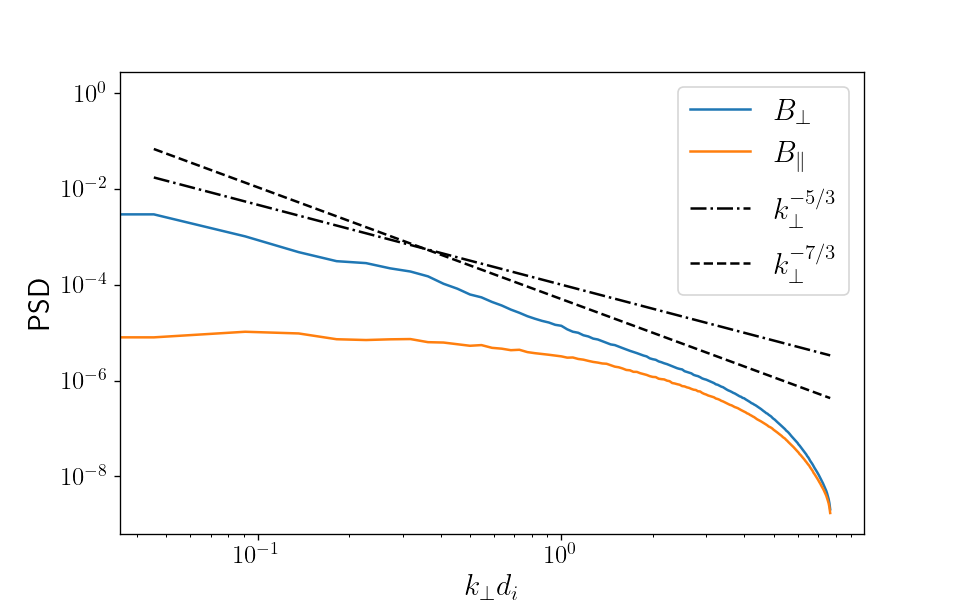
\includegraphics[width=0.95\linewidth,trim=0cm 0cm 0cm 0cm, clip=true]{./Part_3/images_ch3/CGL2_spectre}
% \cprotect\caption{Simu : CGL2. Spectre d'énergie magnétique perpendiculaire et parallèle en fonction de $k_{\perp}d_i$}
% \label{fig:spectre}
% \end{figure}

% Sur le spectre des fluctuations perpendiculaires, on peut remarquer une bosse en $k_{\perp}d_i = 0.3$, cela correspondrait à $\ell_{\perp}/d_i = 21 $. Si l'on regarde sur le triptyque associé à CGL2 (\figref{fig:trip_CGL1-2}), on remarque que cette échelle correspond au début de l'augmentation de $\varepsilon_{\overline{\boldsymbol{\Pi}}}$. 

% Les spectres de CGL5 et CGL6 sont plus complexes à analyser, la contribution des fluctuations parallèles au spectre total prend de l'importance dans la zone Hall, comme on peut le voir pour sur la \figref{fig:spectre_CGL6}. Serait la signature d'une cascade d'ondes magnétosonores ?
% \begin{figure}[!ht]
%  \centering
% 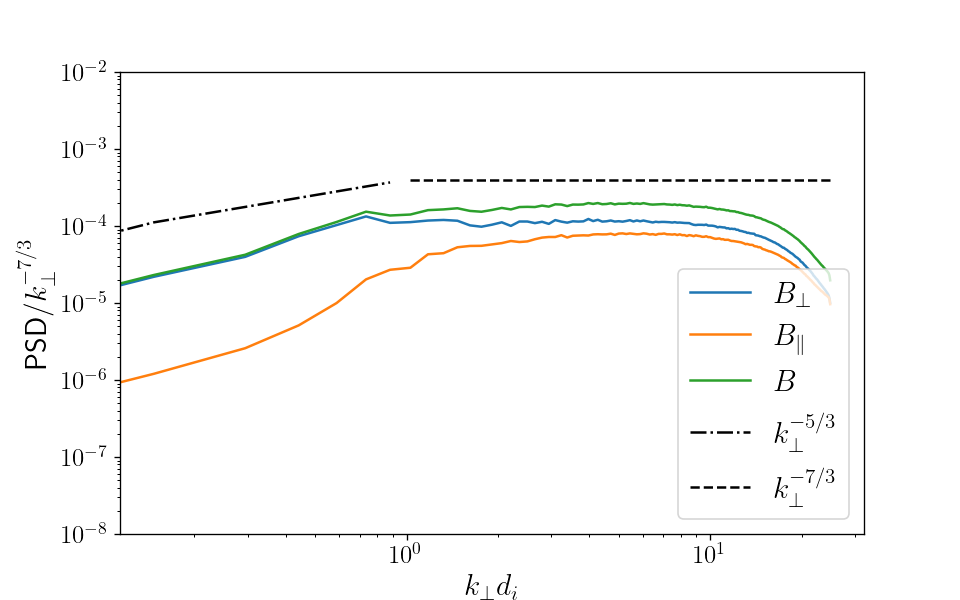
\includegraphics[width=0.95\linewidth,trim=0cm 0cm 0cm 0cm, clip=true]{./Part_3/images_ch3/CGL6_spectre}
% \cprotect\caption{Simu : CGL6. Spectre d'énergie magnétique perpendiculaire et parallèle en fonction de $k_{\perp}d_i$. Le spectre est compensé par la pente $-7/3$ attendue dans la zone inertielle Hall.}
% \label{fig:spectre_CGL6}
% \end{figure}

\chapter{Vers l'étude des simulations Landau-fluides}
\renewcommand\partie{\Partie\ Chapitre \thechapter}
\label{ch-34}

\bigskip
\minitoc  

\cite{ferrand_fluid_2021} ont aussi utilisé des simulations du modèle \acs{LFHPe} prenant en compte un flux de chaleur $\overline{\overline{\boldsymbol{q}}}$ gyrotrope obtenu grâce à une fermeture Landau-fluide présente dans le code utilisé dans cette partie. Il s'est avéré que ces simulations prennent aussi en compte un tenseur de pression électronique de type gyrotrope.
Ces simulations corrigeant les critères d'instabilités tel que le critère miroir afin de refléter le comportement linéaire cinétique, elles pourraient par la suite nous aider à étendre nos interprétations vers les processus cinétiques. 

Dans ce chapitre, nous décrivons les spécificités du modèle implémenté et la loi exacte complète associée. Une première application, préliminaire, à deux simulations, semblent montrer des résultats paradoxaux qui nécessiteront une étude plus fine avant d'en extraire un début d'interprétations. 


\section{Modèle simulé et loi exacte}
\label{sec-341}

Dans ce deuxième lot de simulations, les ions et les électrons sont décrits avec un tenseur de pression gyrotrope. La fermeture utilisée est une fermeture Landau-fluide. Cette fermeture nous rapproche d'un modèle cinétique en prenant en compte l'amortissement Landau linéaire (phénomène cinétique) dans le modèle fluide. Cette correction étant basée sur la relation de dispersion cinétique, les critères d'instabilité seront aussi corrigés pour correspondre aux critères cinétiques. La gyrotropie des électrons impactera d'ailleurs le critère miroir. Les flux de chaleur ioniques et électroniques sont aussi supposés gyrotropes.

Les premières équations du modèle normalisé simulé sont les suivantes, en y faisant apparaître indépendamment les tenseurs de pression ionique et électronique : 
\begin{eqnarray}
\label{eq:mlf_r} \partial_t \rho + \nabla \cdot \left(\rho \boldsymbol{v}\right) &=& 0\\
\label{eq:mlf_v} \partial_t  \boldsymbol{v} + \boldsymbol{v} \cdot \nabla  \boldsymbol{v} - \frac{1}{\rho} \boldsymbol{j} \times \boldsymbol{B} + \frac{1}{\rho} \nabla \cdot \left(\overline{\boldsymbol{P_i}} + \overline{\boldsymbol{P_e}} \right)  &=& 0  \\
\label{eq:mlf_b} \partial_t \boldsymbol{B} - \nabla \times \left( \boldsymbol{v} \times \boldsymbol{B} \right) +  d_i  \nabla \times \left( \frac{1}{\rho} \boldsymbol{j}\times \boldsymbol{B} \right) &=& d_i \nabla \times \left( \frac{1}{\rho} \nabla \left(  p_e\right) \right)  \\
\label{eq:mlf_pperpi} \partial_t  p_{\perp i }  +  \nabla \cdot \left(p_{\perp i } \boldsymbol{v} \right) +  p_{\perp i }\nabla \cdot\boldsymbol{v} -  p_{\perp i } \boldsymbol{b}\boldsymbol{b} : \nabla \boldsymbol{v}  &=& - \frac{1}{2} \left( \text{Tr}(\nabla \cdot \overline{\overline{\boldsymbol{q_i}}}) - \boldsymbol{b}\boldsymbol{b} : \nabla \cdot \overline{\overline{\boldsymbol{q_i}}} \right) \nonumber \\ && \\
\label{eq:mlf_ppari} \partial_t  p_{\parallel i }  +  \nabla \cdot \left(p_{\parallel i } \boldsymbol{v} \right) +  2 p_{\parallel i }  \boldsymbol{b}\boldsymbol{b} : \nabla \boldsymbol{v}  &=&  - \boldsymbol{b}\boldsymbol{b} : \nabla \cdot \overline{\overline{\boldsymbol{q_i}}}   \\
\label{eq:mlf_pperpe} \partial_t  p_{\perp e }  +  \nabla \cdot \left(p_{\perp e } \boldsymbol{v_e} \right) +  p_{\perp e }\nabla \cdot\boldsymbol{v_e} -  p_{\perp e } \boldsymbol{b}\boldsymbol{b} : \nabla \boldsymbol{v_e}  &=&  - \frac{1}{2} \left( \text{Tr}(\nabla \cdot \overline{\overline{\boldsymbol{q_e}}}) - \boldsymbol{b}\boldsymbol{b} : \nabla \cdot \overline{\overline{\boldsymbol{q_e}}} \right) \nonumber \\ && \\
\label{eq:mlf_ppare} \partial_t  p_{\parallel e }  +  \nabla \cdot \left(p_{\parallel e } \boldsymbol{v_e} \right) +  2 p_{\parallel e }  \boldsymbol{b}\boldsymbol{b} : \nabla \boldsymbol{v_e}  &=& - \boldsymbol{b}\boldsymbol{b} : \nabla \cdot \overline{\overline{\boldsymbol{q_e}}} 
\end{eqnarray}

avec $\overline{\boldsymbol{P_{i,e}}} =  \frac{\beta_0}{2} \left(p_{\perp i,e } \overline{\boldsymbol{I}} + \left(p_{\parallel i,e } - p_{\perp i,e }\right) \boldsymbol{b} \boldsymbol{b} \right) $, les tenseurs gyrotropes de pression ionique (i) et électronique (e), $\boldsymbol{b} = \frac{\boldsymbol{B}}{|\boldsymbol{B}|}$, la direction du champ magnétique, $\frac{\beta_0}{2} $ constante provenant de la normalisation des équations, et $\boldsymbol{v_e} = \boldsymbol{v} - d_i \frac{\boldsymbol{j}}{\rho} $ la vitesse électronique. La fermeture est appliquée au niveau du quatrième moment (pour plus d'informations, voir les premières parties de \cite{passot_collisionless_2007}) présent dans les équations de $ \overline{\overline{\boldsymbol{q_i}}}$ et $ \overline{\overline{\boldsymbol{q_e}}}$. L'hypothèse de gyrotropie appliquée aux tenseurs de flux de chaleur implique (avec $s = i,e$) :  
\begin{eqnarray*}
    \boldsymbol{b}\boldsymbol{b} : \nabla \cdot \overline{\overline{\boldsymbol{q_s}}} &\simeq& \nabla \cdot (q_{\parallel s} \boldsymbol{b}) - 2 q_{\perp s} \nabla \cdot \boldsymbol{b}\\
    \frac{1}{2} \left( \text{Tr}(\nabla \cdot \overline{\overline{\boldsymbol{q_s}}}) - \boldsymbol{b}\boldsymbol{b} : \nabla \cdot \overline{\overline{\boldsymbol{q_s}}} \right)  &\simeq&  \nabla \cdot (q_{\perp s} \boldsymbol{b})  + q_{\perp s} \nabla \cdot \boldsymbol{b}
\end{eqnarray*}


L'équation d'énergie interne peut être construite à partir des équations de pression \eqref{eq:mlf_ppari}, \eqref{eq:mlf_pperpi}, \eqref{eq:mlf_ppare}, \eqref{eq:mlf_pperpe} et de la relation $\boldsymbol{v_e} = \boldsymbol{v} - d_i \frac{\boldsymbol{j}}{\rho} $  : 
\begin{eqnarray}
\label{eq:mlf_ui} \partial_t \left(\rho u\right) + \nabla \cdot \left(\rho u \boldsymbol{v} + \boldsymbol{q}\right) +   \left(\overline{\boldsymbol{P_i}} + \overline{\boldsymbol{P_e}} \right): \nabla \boldsymbol{v} &=& \frac{d_i}{2}  \nabla \cdot  \left(\text{Tr} \left(\overline{\boldsymbol{P_e}}\right)  \frac{ \boldsymbol{j}}{\rho} \right) +  d_i \overline{\boldsymbol{P_{e}}} : \nabla \left(\frac{\boldsymbol{j}}{\rho} \right)\nonumber \\ 
\end{eqnarray}
sachant que $\rho u = \frac{\beta_0}{2} \left(p_{\perp i } + \frac{1}{2}p_{\parallel i} + p_{\perp e } + \frac{1}{2}p_{\parallel e} \right) $ et avec $\boldsymbol{q} = \frac{\beta_0}{2} \left(q_{\perp i } + \frac{1}{2}q_{\parallel i} + q_{\perp e } + \frac{1}{2}q_{\parallel e} \right)  \boldsymbol{b}$. 

La loi exacte valable pour ce modèle a pour base \eqref{eq:turb_cpg_elk} à laquelle on doit ajouter la correction Hall \eqref{eq:corr_hall}, la correction dépendant de la pression électronique \eqref{eq:corr_pe} et la correction dépendant des flux de chaleur \eqref{eq:turb_ref_q}. 

Par curiosité, nous l'avons appliquée à deux simulations LF2 et LF3, pour vérifier si l'on pouvait retrouver les conclusions de \cite{ferrand_fluid_2021} à travers les termes dépendant des flux de chaleurs. 

\section{Etude préliminaire des simulations}
\label{sec-342}

Les paramètres initiaux associés à chaque simulation sont donnés dans la \tabref{tab:setups} et la \tabref{tab:setups_hd}. Et, dans la \tabref{tab:stat_LF}, sont repris quelques informations statistiques. Similairement aux simulations \acs{CGLHPe}, les fluctuations de densité  sont faibles, ces simulations sont aussi quasi-incompressibles. 
 \begin{table}[!ht]
\begin{center}
\begin{tabular}{ c|c|c|c|c|c } 
Name & $\rho$ & $a_{pi}$  & $\beta_{\parallel i }$ & $a_{pe}$  & $\beta_{\parallel e }$\\
\hline
%LF1 & $\num{1}\pm \num{0.02}$ & $\num{1.04}\pm \num{0.04}$ & $\num{0.97}\pm \num{0.06}$ & $\num{1.01}\pm \num{0.003}$ & $\num{0.99}\pm \num{0.07}$ \\
LF2 & $\num{1}\pm \num{0.01}$ & $\num{1.05}\pm \num{0.03}$ & $\num{0.97}\pm \num{0.04}$ & $\num{1.01}\pm \num{0.006}$ & $\num{0.98}\pm \num{0.05}$  \\
LF3 & $\num{1}\pm \num{0.08}$ & $\num{1.52}\pm \num{0.31}$ & $\num{0.84}\pm \num{0.30}$ & $\num{0.96}\pm \num{0.04}$ & $\num{1.10}\pm \num{0.42}$  %\\
%LF4 & $\num{1}\pm \num{0.02}$ & $\num{1.07}\pm \num{0.05}$ & $\num{0.94}\pm \num{0.07}$ & $\num{1.07}\pm \num{0.02}$ & $\num{0.92}\pm \num{0.05}$ 
\end{tabular}
\caption{Moyenne et écart-type de la densité, du taux d'anisotropie ionique $a_{pi} = \frac{p_{\perp i}}{p_{\parallel i}}$ et électronique $a_{pe} = \frac{p_{\perp e}}{p_{\parallel e}}$ et des paramètres $\beta_{\parallel i} = \frac{p_{\parallel i}}{p_{m}}$ et $\beta_{\parallel e} = \frac{p_{\parallel e}}{p_{m}}$  pour chaque simulation, à la date $t$. \label{tab:stat_LF}}
\end{center}
\end{table}
\begin{figure}[!ht]
 \centering
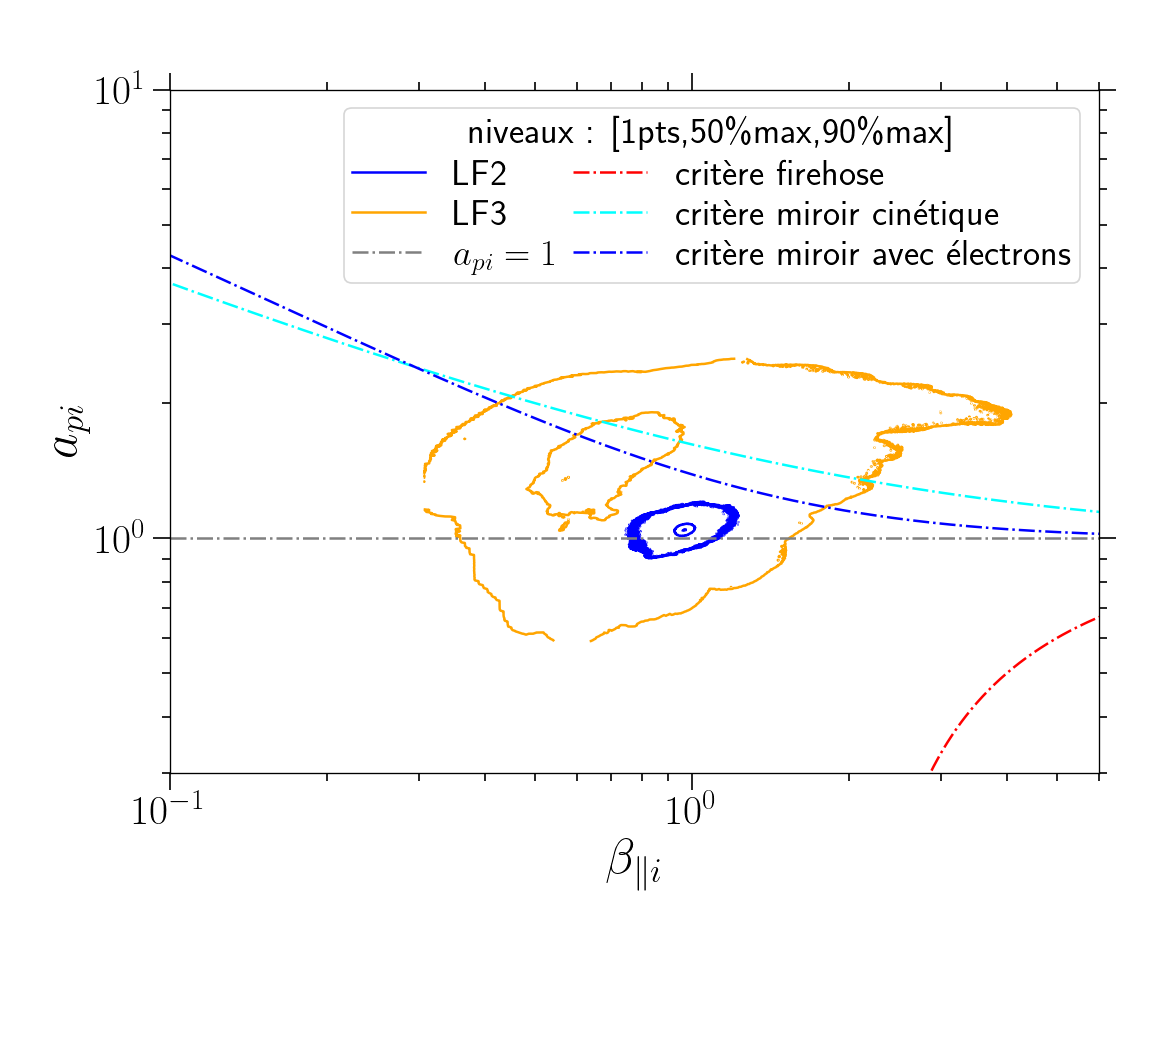
\includegraphics[width=1\linewidth,trim=0cm 2cm 1cm 1cm, clip=true]{./Part_3/images_ch4/diag_simu_LF}
\cprotect\caption{Diagramme $a_{pi}-\beta_{\parallel i}$ contenant l'histogramme \acs{2D} des simulations LF2 et LF3 sous la forme de courbes de niveau centrées sur le couple moyen. Les lignes discontinues correspondent aux critères d'instabilité. Rouge : le critère firehose CGL calculé dans le chapitre \ref{ch-21} et valable dans les modèles cinétique [\cite{hunana_introductory_2019}], il ne prend pas en compte l'effet \acs{Hall}. Cyan : critère miroir cinétique (sans prise en compte de la pression électronique) [\cite{hunana_introductory_2019}]. Bleu : critère miroir proposé par \cite{kuznetsov_mirror_2012}, prenant en compte les électrons gyrotropes et calculé avec $a_{pe} = 1$ et $\beta_{\parallel e } = 1$.}
\label{fig:diag_simu_LF}
\end{figure} 

Les taux d'anisotropie initialisés à $\num{1}$ sont restés proches de 1 et sont moins étalées que ceux des simulations \acs{CGLHPe} CGL2 et CGL3. LF3 montre un étalement plus important similairement à CGL3. Plus d'un tiers des points sont situés dans la zone du diagramme située du côté instable du critère miroir. Deux critères miroirs sont donnés. Le premier en cyan correspond au critère cinétique obtenue en corrigeant le facteur 6 du critère CGL [\cite{galeev_mhd_1983,ferriere_mixed_2002,hunana_introductory_2019}]. Le second, en bleu, est aussi un critère miroir cinétique mais prenant en compte l'anisotropie de pression électronique. Ce critère est dérivé dans l'article [\cite{kuznetsov_mirror_2012}]. Il est ici représenté en considérant $a_{pe} = 1$ et $\beta_{\parallel e } = 1$. 

Les simulations LF pourrait donc permettre une étude fine de l'impact des instabilités cinétiques sur la cascade turbulente. Mais, en première application de la loi exacte étendue et par curiosité, nous avons d'abord cherché à retrouver les résultats de \ac{F21}. 



\section{Premières applications de la loi exacte \acs{LFHPe}}
\label{sec-343}

Pour les simulations LF2 et LF3, l'extraction d'échantillons de temps consécutifs n'a pas encore été fait. On ne fera donc pas apparaître le niveau $\zeta$ dans les résultats qui suivent qui sont préliminaires.

L'une des questions que nous nous sommes posés est : est-ce que l'on retrouve la décroissance associée au flux de chaleur par \ac{F21} ? On a alors calculé le taux de cascade total dans LF2 et LF3 avec ($\varepsilon|\nabla \cdot \boldsymbol{q} \neq 0$) et sans ($\varepsilon|\nabla \cdot \boldsymbol{q} = 0$) la contribution du flux de chaleur. Les résultats sont montrés sur la figure \figref{fig:LF_q}.
\begin{figure}[!ht]
 \centering
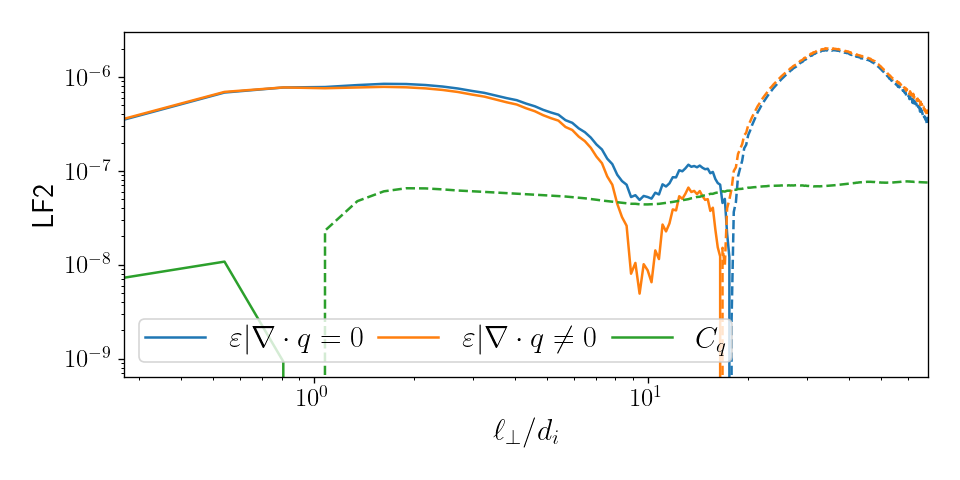
\includegraphics[width=0.9\linewidth,trim=1cm 1cm 0cm 1cm, clip=true]{./Part_3/images_ch4/LF2_q}
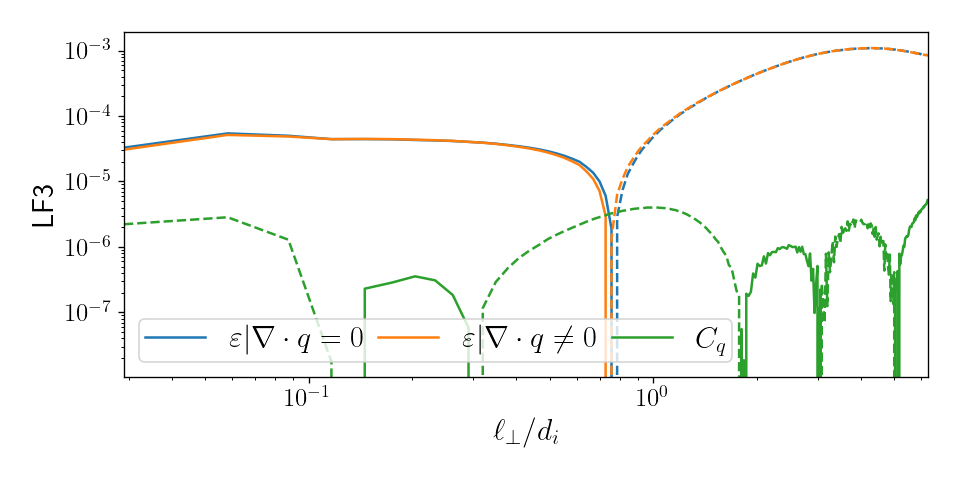
\includegraphics[width=0.9\linewidth,trim=1cm 1cm 0cm 1cm, clip=true]{./Part_3/images_ch4/LF3_q}
\cprotect\caption{Taux de cascade calculé en prenant en compte la contribution de flux de chaleur et en l'omettant.}
\label{fig:LF_q}
\end{figure} 
On remarque que la contribution du flux de chaleur ($C_q$, vert) semble négligeable même aux plus petites échelles. On ne retrouve donc pas la décroissance observée en allant vers les petites échelles que l'on s'attendait à voir en ne le prenant pas en compte en accord avec les résultats de \ac{F21}.

Afin de vérifier si une erreur ne s'était pas introduite dans notre calcul. Nous avons calculé la loi exacte la plus proche de la loi incompressible observée par \cite{ferrand_fluid_2021}, c'est-à-dire la loi Hall-MHD (HMHD) en n'y prenant en compte que les contributions isotropes des tenseurs de pression ionique et électronique, les termes dépendant de l'anisotropie de pression, du terme \acs{Pe} de la loi d'Ohm ou des flux de chaleur étant nouveaux dans l'estimation du taux de cascade. Ce taux de cascade est représenté en orange sur la figure \figref{fig:LF_detail}. On retrouve bien le résultat de \ac{F21} avec la décroissance en allant vers les petites échelles. Ayant deux résultats semblant en contradiction, $\varepsilon|\nabla \cdot \boldsymbol{q}$ (bleu) et $\varepsilon_{HMHD}$, j'ai ajouté une à une les nouvelles contributions afin de comprendre ce qu'il se passait. 

\begin{figure}[!ht]
 \centering
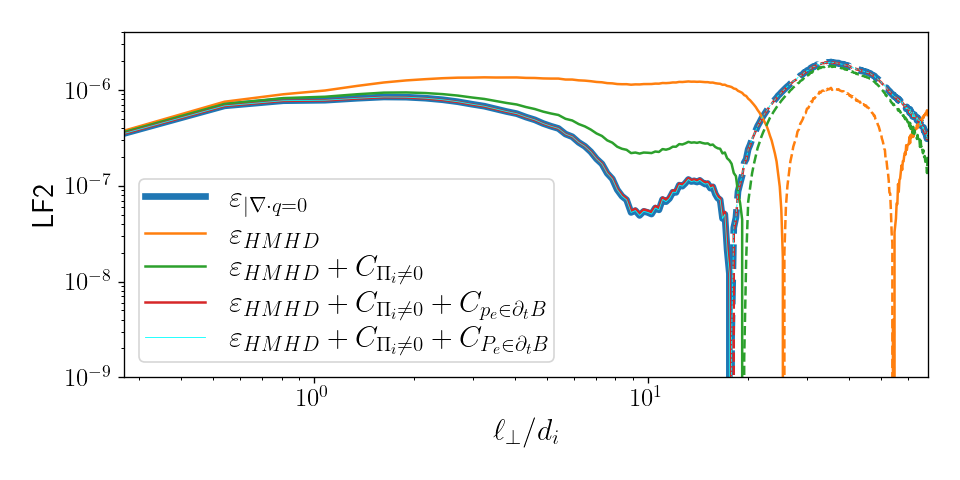
\includegraphics[width=1\linewidth,trim=1cm 1cm 0cm 1cm, clip=true]{./Part_3/images_ch4/LF2_detail}
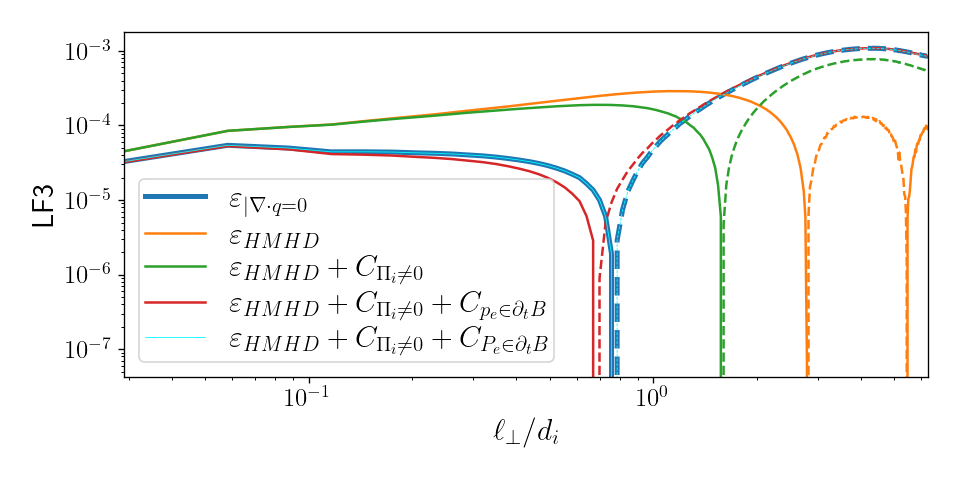
\includegraphics[width=1\linewidth,trim=1cm 1cm 0cm 1cm, clip=true]{./Part_3/images_ch4/LF3_detail}
\cprotect\caption{Taux de cascade calculé en prenant petit à petit en comptes les nouvelles contributions afin d'identifier quelles contributions impactent le taux de cascade \acs{LFHPe}. Le but étant de retrouver le taux de transfert  non linéaire total de ces simulations (courbe bleue épaisse) en partant d'une loi \acs{MHDH} (orange). Etape 1 (vert) : ajout de l'anisotropie de pression ionique. Etape 2 (rouge) : ajout de la contribution de pression électronique isotrope. Etape 3 (cyan) : prise en compte des anisotropies de pression électronique. Le taux de référence est quasiment retrouvé en ajoutant l'anisotropie de pression ionique et la pression isotrope électronique.}
\label{fig:LF_detail}
\end{figure} 
 Tout d'abord, on prend en compte l'anisotropie de pression des ions et des électrons (en gardant une loi d'Ohm Hall-MHD), le résultat correspond à la courbe verte. Le niveau du taux de cascade commence à s'affaisser aux échelles a priori inertielles, et à augmenter dans les échelles d'injections. Ces ajouts sont dominés par la pression ionique.

Ensuite, on ajoute la contribution de la pression électronique isotrope associée au terme \acs{Pe} de la loi d'Ohm, cela donne la courbe rouge. Le résultat est alors très proche du résultat voulu. La composante anisotrope des tenseurs de pression dans ce terme (résultat cyan) s'avère faible pour LF2 et influe un peu plus pour LF3. Le résultat  $\varepsilon|\nabla \cdot \boldsymbol{q}$ observé sur la \figref{fig:LF_q}
est ainsi retrouvé.

Ce résultat semble paradoxal face aux conclusions de \ac{F21}. Dans cet article, ils concluent en comblant la décroissance du taux de cascade par une estimation d'un taux de dissipation dû à l'amortissement Landau, remontant ainsi le niveau du taux de cascade dans la zone inertielle. De notre côté, on observe plutôt un affaissement du niveau du taux dû à la prise en compte de l'anisotropie de pression ionique ainsi que du tenseur de pression électronique dans l'équation d'induction. Ces résultats obtenus très récemment semblent venir questionner la méthode d'obtention du taux de dissipation par effet Landau utilisée par \ac{F21} ou notre interprétation de la contribution du flux de chaleur dans le taux de cascade et demande une analyse plus fine que ce qui a pu être fait jusqu'à présent. 


\chapter*{Conclusion}
 \addcontentsline{toc}{chapter}{Conclusion}
 \adjustmtc
\renewcommand\partie{\Partie\ CONCLUSION}
\label{ch-35}

\bigskip
\minitoc  

Cette Partie \ref{part_3} contient l'état actuel de notre étude numérique de l'effet de l'anisotropie de pression sur la cascade turbulente. 

Dans le Chapitre \ref{ch-31}, nous présentons le code qui nous a permis d'obtenir les données dans lesquelles l'étude des lois exactes est effectuée ainsi que notre méthode de post-traitement. Cette méthode reposant sur l'usage de la transformée de Fourier, n'est à notre connaissance pas utilisée par la communauté. 

Dans le Chapitre \ref{ch-32}, sont exposées les étapes ayant permis la validation de notre code ainsi qu'une étude de l'apport de notre méthode sur une méthode utilisée couramment consistant à décrire l'espace des échelles par un ensemble réduit de vecteurs. En se basant sur nos connaissances du code et sur le travail analytique de la Partie \ref{part_2}, nous y développons une méthode d'obtention de l'erreur numérique s'appliquant sur nos résultats ainsi qu'une analyse approfondie de nos sources d'erreur. 

Ainsi armé de ces outils, nous avons attaqué l'analyse complète des simulations utilisées par \cite{ferrand_fluid_2021} afin de valider l'apport de notre extension gyrotrope de la théorie des lois exactes et d'affiner notre compréhension de l'effet de l'anisotropie de pression sur la turbulence. Le Chapitre \ref{ch-33} contient une analyse préliminaire des simulations du modèle \acs{CGLHPe}. Cette étude valide l'apport de notre extension en particulier le poids, dans des simulations incompressibles, du terme survivant dans la limite incompressible et qui a fait l'objet du Chapitre \ref{ch-22}. Cependant, l'interprétation de ses résultats est encore sujette à discussion et nécessitera quelques analyses complémentaires. Le Chapitre \ref{ch-34} contient une ouverture vers l'application de nos résultats analytiques et de nos méthodes dans des simulations plus complexes prenant en compte l'effet Landau-fluide. De telles simulations rapprochent le comportement du système de celui décrit par un modèle cinétique en captant partiellement l'effet Landau linaire. Les tout premiers résultats questionnent notre interprétation de l'impact du flux de chaleur sur la cascade turbulente, et nécessiteront une analyse plus fine avant de mener à un début d'interprétation. 






